\documentclass[12pt,a4paper]{article}
%-------------------------------------------
%---Packages--------------------------------
%-------------------------------------------
\usepackage[utf8]{inputenc}
%\usepackage[T1]{fontenc}
%\usepackage{txfonts}
\usepackage{amsmath}
\usepackage{amsthm}
\usepackage{amsfonts}
\usepackage{array}
\usepackage{amssymb}
\usepackage{blindtext}
\usepackage{caption}
\usepackage{color}
\usepackage{csquotes}	    %
\usepackage{enumitem}	    %pour mieux bosser avec les listes. ajoute option label
\usepackage[yyyymmdd]{datetime}        %pour définir date custom
\usepackage{etaremune}
\usepackage{environ}
\usepackage{fancybox}
\usepackage{fancyhdr} 	    % Custom headers and footers
\usepackage{fancyref}
%\usepackage{float}
\usepackage{floatrow}       %float and floatrow can't be together...
\usepackage{gensymb}
\usepackage{graphicx}
\usepackage[colorlinks=true, linkcolor=purple, citecolor=cyan]{hyperref}
\usepackage{footnotebackref}
\usepackage{lipsum}
\usepackage{mathtools}
\usepackage{multicol}	    %gérer plusieurs colonnes
\usepackage{setspace}
\usepackage{subcaption}
\usepackage{todonotes}	    %Bonne gestion des TODOs
%TODO commenté pour tester l'utilité... à voir% \usepackage[tc]{titlepic}      %Permet de mettre une image en page de garde
\usepackage{tikz}	    % Pour outil de dessin puissant
\usepackage{ulem}	    %underline sur plusieurs lignes (avec \uline{})
\usepackage{vmargin} 	    %gestion des marges, avec dans l'ordre : gauche, haut, droit, bas, en-tête, entre en-tête et texte, bas de page, hauteur entre bas de page et texte
\usepackage{wrapfig}
\usepackage{xcolor}
\usepackage{xparse}                    %Pour utiliser NewDocumentCommand et des arguments 'mmooo'
%\usepackage{fullpage} 	    %supprime toutes les marges allouées aux notes, aussi en haut et en bas

%\ExplSyntaxOn
\pagestyle{fancyplain}	    %Makes all pages in the document conform to the custom headers and footers

%-------------------------------------------
%---Document Commands-----------------------
%---------------------------{----------------
\NewDocumentCommand{\framecolorbox}{oommm}
 {% #1 = width (optional)
  % #2 = inner alignment (optional)
  % #3 = frame color
  % #4 = background color
  % #5 = text
  \IfValueTF{#1}%
   {\IfValueTF{#2}%
    {\fcolorbox{#3}{#4}{\makebox[#1][#2]{#5}}}%
    {\fcolorbox{#3}{#4}{\makebox[#1]{#5}}}%
   }%
   {\fcolorbox{#3}{#4}{#5}}%
 }%
%------------------------------------------------
%------------------ENGLISH----------------------
%----------------------------------------------

\NewDocumentCommand{\epflTitle}{mO{Olivier Cloux}O{\today}O{Notes de Cours en}D<>{../../Common}}%Arguments : Matière, Auteur, Date, Titre du doc
{
\begin{titlepage}
    \vspace*{\fill}
    \begin{center}
        \normalfont \normalsize
        \textsc{Ecole Polytechnique Fédérale de Lausanne} \\ [25pt] % Your university, school and/or department name(s)
        \textsc{#4} %Titre du doc
        \\ [0.4 pt]
        \horrule{0.5pt} \\[0.4cm] % Thin top horizontal rule
        \huge #1 \\ % Matière
        \horrule{2pt} \\[0.5cm] % Thick bottom horizontal rule
        
\includegraphics[width=8cm]{#5/EPFL_logo}
        ~\\[0.5 cm]
        \small\textsc{#2}\\[0.4cm]
        \small\textsc{#3}\\
        ~\\
        ~\\
        
\includegraphics[scale=0.5]{#5/creativeCommons}
    \end{center}
    \vspace*{\fill}
\end{titlepage}
}


%-------------------------------------------
%-------------MATH NEW COMMANDS-------------
%-------------------------------------------
\newcommand{\somme}[2]{\ensuremath{\sum\limits_{#2}^{#1}}}
\newcommand{\produit}[2]{\ensuremath{\prod\limits_{#2}^{#1}}}
\newcommand{\limite}{\lim\limits_}
\newcommand{\llimite}[3]{\limite{\substack{#1 \\ #2}}\left(#3\right)}	%limites à deux condiitons
\newcommand{\et}{\mbox{ et }}
\newcommand{\deriv}[1]{\ensuremath{\, \mathrm d #1}}	%sigle dx, dt,dy... des dérivées/intégrales
%\newcommand{\fx}{\ensuremath{f'(\textbf{x}_0 + h}}
\newcommand{\ninf}{\ensuremath{n \to \infty}}	       %pour les limites : n tend vers l'infini
\newcommand{\xinf}{\ensuremath{x \to \infty}}	       %pour les limites : x tend vers l'infini
\newcommand{\infint}{\ensuremath{\int_{-\infty}^{\infty}}}
\newcommand{\xo}{\ensuremath{x \to 0}}									%x to 0
\newcommand{\no}{\ensuremath{n \to 0}}									%n zéro
\newcommand{\xx}{\ensuremath{x \to x}}									%x to x
\newcommand{\Xo}{\ensuremath{x_0}}										%x zéro
\newcommand{\X}{\ensuremath{\mathbf{X}} }
\newcommand{\A}{\ensuremath{\mathbf{A}} }
\newcommand{\R}{\ensuremath{\mathbb{R}} }								%ensemble de R
\newcommand{\rn}{\ensuremath{\mathbb{R}^n} } 							%ensemble de R de taille n
\newcommand{\Rm}{\ensuremath{\mathbb{R}^m} }  							%ensemble de R de taille m
\newcommand{\C}{\ensuremath{\mathbb{C}} }
\newcommand{\N}{\ensuremath{\mathbb{N}} }
\newcommand{\Z}{\ensuremath{\mathbb{Z}} }
\newcommand{\Q}{\ensuremath{\mathbb{Q}} }
\newcommand{\rtor}{\ensuremath{\R \to \R} }
\newcommand{\pour}{\mbox{ pour }}
\newcommand{\coss}[1]{\ensuremath{\cos\(#1\)}}						%cosinus avec des parenthèses de bonne taille (genre frac)
\newcommand{\sinn}[1]{\ensuremath{\sin\(#1\)}}					%sinus avec des parentèses de bonne taille (genre frac)
\newcommand{\txtfrac}[2]{\ensuremath{\frac{\text{#1}}{\text{#2}}}}		%Fractions composées de texte
\newcommand{\evalfrac}[3]{\ensuremath{\left.\frac{#1}{#2}\right|_{#3}}}
\renewcommand{\(}{\left(}												%Parenthèse gauche de taille adaptive
\renewcommand{\)}{\right)}
\newcommand{\longeq}{=\joinrel=}												%Parenthèse droite de taille adaptive


%-------------------------------------------------------
%------------------MISC NEW COMMANDS--------------------
%-------------------------------------------------------
\newcommand{\degre}{\ensuremath{^\circ}}
%\newdateformat{\eudate}{\THEYEAR-\twodigit{\THEMONTH}-\twodigit{\THEDAY}}



%-------------------------------------------------------
%------------------TEXT NEW COMMANDS--------------------
%-------------------------------------------------------
\newcommand{\ts}{\textsuperscript}
\newcommand{\evid}[1]{\textbf{\uline{#1}}}        %mise en évidence (gras + souligné)



%\newcommand{\Exemple}{\underline{Exemple}}
\newcommand{\Theoreme}{\underline{Théorème}}
\newcommand{\Remarque}{\underline{Remarque}}
\newcommand{\Definition}{\underline{Définition} }
\newcommand{\skinf}{\sum^{\infty}_{k=0}}
\newcommand{\combi}[2]{\ensuremath{\begin{pmatrix} #1 \\ #2 \end{pmatrix}}}	%combinaison parmi 1 de 2
\newcommand{\intx}[3]{\ensuremath{\int_{#1}^{#2} #3 \deriv{x}}}				%intégrale dx
\newcommand{\intt}[3]{\ensuremath{\int_{#1}^{#2} #3 \deriv{t}}}				%intégrale dy
\newcommand{\misenforme}{\begin{center} Mis en forme jusqu'ici\\ \line(1,0){400}\\ normalement juste, mais à améliorer depuis ici\end{center}}	%raccourci pour mise en forme
\newcommand*\circled[1]{\tikz[baseline=(char.base)]{
            \node[shape=circle,draw,inner sep=1pt] (char) {#1};}}			%pour entourer un chiffre
\newcommand{\horrule}[1]{\rule{\linewidth}{#1}} 				% Create horizontal rule command with 1 argument of height

\theoremstyle{definition}
\newtheorem{exemp}{Exemple}
\newtheorem{examp}{Example}


%-------------------------------------------
%---Environments----------------------------
%-------------------------------------------
\NewEnviron{boite}[1][0.9]{%
	\begin{center}
		\framecolorbox{red}{white}{%
			\begin{minipage}{#1\textwidth}
 	 			\BODY
			\end{minipage}
		}
	\end{center}
}
\NewEnviron{blackbox}[1][0.9]{%
	\begin{center}
		\framecolorbox{black}{white}{%
			\begin{minipage}{#1\textwidth}
 	 			\BODY
			\end{minipage}
		}
	\end{center}
}
\NewEnviron{exemple}[1][0.8]{%
    \begin{center}
        \framecolorbox{white}{gray!20}{%
            \begin{minipage}{#1\textwidth}
                \begin{exemp}
                    \BODY
                \end{exemp}
            \end{minipage}
        }
    \end{center}
}
\NewEnviron{suiteExemple}[1][0.8]{%
    \begin{center}
        \framecolorbox{white}{gray!20}{%
            \begin{minipage}{#1\textwidth}
                \BODY
            \end{minipage}
        }
    \end{center}
}
\NewEnviron{colExemple}[1][0.8]{%
    \begin{center}
        \framecolorbox{white}{gray!20}{%
            \begin{minipage}{#1\columnwidth}
                \begin{exemp}
                    \BODY
                \end{exemp}
            \end{minipage}
        }
    \end{center}
}
\NewEnviron{example}[1][0.8]{%
    \begin{center}
        \framecolorbox{white}{gray!20}{%
            \begin{minipage}{#1\textwidth}
                \begin{examp}
                    \BODY
                \end{examp}
            \end{minipage}
	}
    \end{center}
}
\NewEnviron{systeq}[1][l]{
			\begin{center}
				$\left\{\begin{array}{#1}
					\BODY
				\end{array}\right.$
			\end{center}
 }





%-------------------------------------------
%---General settings-----------------------
%-------------------------------------------
\renewcommand{\headrulewidth}{1pt}										%ligne au haut de chaque page
\renewcommand{\footrulewidth}{1pt}										%ligne au pied de chaque page
\setstretch{1.6}
\author{Olivier Cloux}

\renewcommand{\contentsname}{Table des Matières}
\usepackage{todonotes}
\usepackage{fixme}
\newcommand{\I}{\text{Î} }
\newcommand{\U}{\text{Û} }
\newcommand{\uz}{\uline{Z} }
\newcommand{\ux}{\uline{X} }
\newcommand{\uy}{\uline{Y} }
\newcommand{\ui}{\uline{I} }
\newcommand{\uu}{\uline{U} }
\newcommand{\uv}{\uline{V} }
\newcommand{\us}{\uline{S} }
\newcommand{\up}{\uline{P} }
\newcommand{\ua}{\uline{A} }
\newcommand{\ub}{\uline{B} }
\newcommand{\uc}{\uline{C} }
\newcommand{\ud}{\uline{D} }
%%TODO : Supprimer quand plus de todo %%%%%
%\marginparwidth = 75pt
%\textwidth = 400pt
%%%%%%%%%%%%%%%%%%%%%%%%%%%%%%%%%%%%%%%%%%%%
\begin{document}
\setstretch{1}
\epflTitle{Circuits et Systèmes I}[Olivier Cloux][Automne 2015]
\begin{multicols}{2}
	\tableofcontents
\end{multicols}

\section{Notions de base}
\label{section: notion de base}
Rappelons nous de la définition d'un circuit électrique. Un circuit est une interconnexion entre éléments (composants) électriques. Ils servent à un transfert d'énergie ou de communication d'un point à un autre. Tout circuit est formé de branches ---câbles--- et n\oe uds ---séparation d'un câble en 2 ou plus--- afin de permettre la circulation d'électricité. 

Nous avons à notre disposition une série d'éléments soit linéaires, que sont les résistances, inductances, capacités, soit actifs (sources), que sont les sources de tension et de courant.

Nous exprimons nos circuits en fonction de deux grandeurs de base : le courant et la tension.

\subsection{Charge}
\label{subsection: base charge}
La charge est une propriété des particules atomiques qui composent la matière. Elle se mesure en \textbf{Coulomb} :
\begin{equation}
	1C = \frac{1}{2.602\cdot10^{-19}} = 6.24\cdot 10^{18} \text{ électrons}
	\label{equ: definition charge}
\end{equation}
Cela nous permet de noter la valeur de la charge élémentaire, soit celle d'un électron, qui est de :
\[e^{-} = -1,602 \cdot 10^{-19}\]

\subsection{Courant}
\label{subsection: base courant}
Nous l'avons dit précédemment, une des manière d'exprimer un réseau est en fonction du \uline{courant}. Le courant électrique est le taux de variation de la charge, qui se mesure en \textbf{Ampère [A]}. Autrement dit, il s'agit de la différence (le passage) de charges pendant un temps donné. Mathématiquement, la relation entre la \uline{charge $q$} et le courant $i$ s'exprime :
\begin{equation}
	i(t) = \frac{\deriv{q}}{\deriv{t}} \qquad q(t) = \int_0^t i(\tau) \deriv{\tau}
	\label{equ: relation charge courant}
\end{equation}
Notons que le sens du courant dans un fil est donné par le mouvement des charges positives. 

Comme exprimé à la Figure \ref{figs: continu/alternatif} courant peut être de 2 natures: 
\begin{itemize}
	\item 	Il peut être \uline{continu} ---constant--- et est alors noté $I$ car il le dépend pas du temps. Sa valeur est constante.
	\item 	Il peut être \uline{alternatif} ---variable--- et sera noté $i(t)$ pour indiquer que sa valeur dépend du temps. Cette forme est obtenue en changeant le courant périodiquement de sens, ce qui donne lieu à des graphes périodiques, souvent sinusoïdaux. Dans le cas sinusoïdal, la tension (respectivement le courant) oscille entre deux valeurs \uline{de crête}, $\U$ et $-\U$ (respectivement $\I$ et $-\I$). Cela permet une définition plus fine :
	\begin{equation}
		u(t) = \U\sin(\omega t) \quad i(t) = \frac{1}{R}u(t) = \I \sin(\omega t)		
	\end{equation}
\end{itemize}
\begin{figure}[h]
	\centering
	\begin{subfigure}{0.3\textwidth}
		\centering
		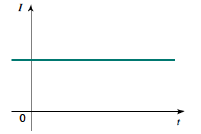
\includegraphics[scale=1]{images/continu}
		\label{subfig: continu}
	\end{subfigure}
	\begin{subfigure}{0.6\textwidth}
		\centering
		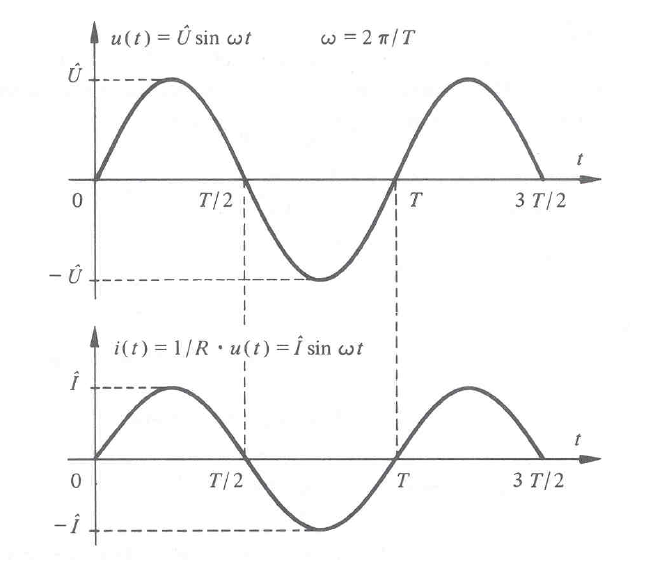
\includegraphics[scale=0.5]{images/regimes}
		\label{subfig: alternatif}
	\end{subfigure}
	\caption{Des graphes de courants, respectivement continu et alternatif}
	\label{figs: continu/alternatif}
\end{figure}

\subsection{Tension}
\label{subsection: base tension}
L'autre manière de quantifier un réseau est par la \uline{tension}. Mais qu'est-ce ? Le déplacement des électrons dans un conducteur suivant une direction particulière exige un certain travail ou transfert d'énergie. Ce travail est accompli par une force extérieure à la charge, assurée par une source d'alimentation et appelée \textit{force électromotrice}, \textit{tension} ou encore \textit{différence de potentiel}. Nous pouvons comme cela définir la tension\footnote{L'appellation \textit{différence de potentiel} est aussi fréquemment utilisée} $v_{ab} \sim u_{ab}$ entre deux points d'un circuit comme ``l'énergie nécessaire pour déplacer une charge électrique unitaire du point \textit{a} au point \textit{b}''. Cette tension se mesure en \textbf{Voltes [V]}. Mathématiquement :
\begin{equation}
	u_{ab} = \frac{\deriv{w}}{\deriv{q}}
	\label{equ: definition tension}
\end{equation}
Avec $w$ l'énergie (J) et $q$ la charge (C). 
Le volt équivaut à la différente de potentiel qui existe entre deux points d'un conducteur parcouru par un courant de 1A lorsque la puissance dissipée entre ces points est de 1W
La tension est toujours définie entre deux points du circuit, $a$ et $b$. Si nous voulons comparer des points entre eux, nous définissons une masse, un point tel que ``ici le potentiel est de 0 par rapport au reste''. Deux cas sont possibles : si $u_{ab} > 0$ alors le potentiel en $a$ est plus grand que celui en $b$. Si $u_{ab} < 0$, le constat inverse se pose.

Petite parenthèse, qui ne sera pas exploitée dans ce cours : il est aussi possible de définir la tension entre $a$ et $b$  comme l'intégrale du champs électrique entre ces points :
\[u_{ab} = \int_a^b \vec{E} \cdot \vec{\deriv{l}}\]

\subsection{Puissance et énergie}
\label{subsection: puissance energie}
Les concepts traités jusqu'ici parlent d'énergie. Mais qui dit énergie, dit forcément puissance. De manière générale, la puissance est la vitesse avec laquelle on consomme de l'énergie. Pour cela, on utilise le \textbf{Watt [W]} ; un watt correspond au transfert de 1 joule d'énergie pendant une seconde. Mathématiquement :
\begin{equation}
	p= \frac{\deriv{w}}{\deriv{t}} = \frac{\deriv{w}}{\deriv{q}} \cdot \frac{\deriv{q}}{\deriv{t}} = u\cdot i
	\label{equ: definition puissance}
\end{equation}
Il est possible de calculer la puissance dite instantanée $p(t)$ où la puissance moyenne $P$, qui correspond à la moyenne de la puissance instantanée. Mathématiquement :
\begin{equation}
	p(t) = u(t)\cdot i(t) \qquad P = \frac{1}{t_2-t_1}\int_{t_1}^{t_2} u(t)i(t) \deriv{t} = \frac{1}{T}\int_0^T u(t)i(t)\deriv{t}
	\label{equ: definition puissance p=ui}
\end{equation}

De manière réciproque, l'énergie absorbée ou fournie par un élément pendant un intervalle de temps $t$ est 
\begin{equation}
	w(t) = \int_0^t p(\tau)\deriv{\tau}
	\label{equ: definition energie}
\end{equation}
Notons également que, par la loi de conservation de l'énergie, la somme algébrique de la puissance dans un circuit doit être zéro à tout instant ; soit : $\sum P = 0$

\subsection{Les éléments passifs}
\label{subsection: elements passifs}
\subsubsection{Résistance}
\label{subsubsection : resistance}
Un câble n'est pas parfait. Il consomme également de l'énergie, chauffe, bref constitue une \textbf{résistance} dans le trajet de l'électricité. Soit un câble de longueur $L$, section $a$ et résistivité $\rho$. Définissons aussi $J$ comme la densité de courant $\left[\frac{A}{m^2}\right]$. La loi d'Ohm se définit telle que :
\begin{equation}
	E = \rho J \to \et R = \rho \frac{L}{a}
	\label{equ: Ohm}
\end{equation}
Mais surtout, la loi la plus essentielle, est celle-ci :
\begin{boite}[0.7]
	\textbf{Résistance :}
	\begin{equation}
		R = \frac{u}{i}
		\label{equ: URI}
	\end{equation}
	La valeur d'une résistance est mesurée en \textbf{Ohm [$\Omega$]}
\end{boite}
avec $u$ = la tension mesurée aux bornes du câble et $i$ le courant traversant la portion de câble. Mais les résistances ne se trouvent pas seulement dans les câbles. Il s'agit également d'un élément physique propre. 

Ainsi, la résistance est extrêmement liée au courant et à la tension. Le but d'une résistance est de réduire la tension qui en sort. Cette énergie qu'on supprime doit bien partir quelque part. Elle est alors dissipée sous forme de chaleur pendant une durée $t$. 
\[w_R(t) =  R  \int_0^t i^2(\tau) \deriv{\tau} = \frac{1}{R}\int_0^tu^2(\tau)\deriv{\tau}\]
En revanche, si le régime est continu, nous pouvons simplifier : 
\[i(t) = I,\ u(t) = U \to w_R(t) = RI^2t = \frac{U^2t}{R}\]
Il est parfois plus aisé de représenter une résistance par son inverse. C'est le rôle de la conductance ; cette grandeur est définie exactement par 
\begin{boite}
	\textbf{Conductance :}
	\begin{equation}
		G = \frac{1}{R} \iff i(t) = Gu(t)
	\end{equation}
	La conductance s'exprime en \textbf{Siemens [S]}
\end{boite}

\subsubsection{Capacité}
\label{subsubsection: capacite}
La capacité est un élément qui se charge avec le temps, et se définit en fonction du courant et des charges
\begin{equation}
	q(t) = C u(t)
\end{equation}
Également, sachant que le courant est le débit de charges (c.f. équation \ref{equ: relation charge courant}), nous pouvons également dire que
\begin{boite}
	\textbf{Capacité}
	\begin{equation}
		i(t) = C \frac{d{u}}{d{t}} \quad u(t) = \frac{1}{C}\int_{-\infty}^t i(\tau)\deriv{\tau} = u(0) + \frac{1}{C}\int_0^t i(\tau)\deriv{\tau}
		\label{equ: capacite}
	\end{equation}	
	La valeur C de la capacité s'exprime en \textbf{farad [F]}
\end{boite}
\uline{En régime continu, la capacité agit comme un circuit ouvert}. En revanche, dans un le cas particulier du régime sinusoïdal, l'équation \ref{equ: capacite} peut se simplifier comme
\begin{equation}
	\I = \omega C \U
\end{equation}

%%%%%%%%%%%%%%%%%%%%%%%%%%%%%%%%%%%%%%%%%%%%%%%%%%%%%%%%%%%%%%%%%%%%%%%%%%%%%
%%%%%%%%%%%%%%%%%%%%%Compléter peut être ?%%%%%%%%%%%%%%%%%%%%%%%%%%%%%%%%%%%
%%%%%%%%%%%%%%%%%%%%%%%%%%%%%%%%%%%%%%%%%%%%%%%%%%%%%%%%%%%%%%%%%%%%%%%%%%%%%

\subsubsection{Inductance}
\label{subsubsection: inductance}
Un élément un peu ``opposé à la capacité'' car il répond à la loi suivante :
\begin{boite}
	\textbf{Inductance :}
	\begin{equation}
		u(t) = L\frac{d{i}}{d{t}}
	\end{equation}
	L'unité de l'inductance est le \textbf{Henry [H]}
\end{boite}
Les inductances peuvent être \textbf{couplées} ; on les appelle aussi \uline{mutuelles} :
\begin{multicols}{2}
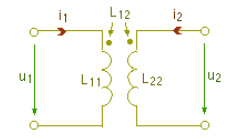
\includegraphics[scale=0.8]{images/inductance_couplee.png}~\columnbreak
~\\
\begin{align}
    u_1 = L_{11}\frac{di_1}{dt} + L_{12}\frac{di_2}{dt}\\
    u_2 = L_{12}\frac{di_1}{dt} + L_{22}\frac{di_2}{dt}
\end{align}

\end{multicols}%%%%%%%%%%%%%%%%%%%%%%%%%%%%%%%%%%%%%%%%%%%%%%%%%%%%%%%%%%%%%%%%%%%%%%%%%%%%%
%%%%%%%%%%%%%%%%%%%%%Compléter peut être ?%%%%%%%%%%%%%%%%%%%%%%%%%%%%%%%%%%%
%%%%%%%%%%%%%%%%%%%%%%%%%%%%%%%%%%%%%%%%%%%%%%%%%%%%%%%%%%%%%%%%%%%%%%%%%%%%%

\subsubsection{Court-circuits}
Nous avons mentionné plus tôt qu'un câble opposait une résistance au courant, en l'empêchant de circuler correctement. Regardons les cas limites :

Si nous faisons tendre cette résistance vers \textit{zéro}, deux points sont en \textbf{court-circuit}. En pratique (et dans nos dessins), cela revient a les relier par un simple fil, sans résistance ou élément supplémentaire.

Si nous faisons tendre cette résistance vers \textit{l'infini}, deux points sont alors en \textbf{circuit ouvert}. En pratique, comme aucun courant ne peut passer par là, cela revient à simplement supprimer le fil (et tous les éléments) entre deux points.

\subsection{Éléments actifs}
\label{subsection: elements actifs}
Il s'agit ici des deux éléments qui apportent de l'énergie au système. Les autres ne faisaient que la modifier, stocker, dissiper. Nous allons parler des \textit{sources}

\subsubsection{Source de Tension}
\label{subsubsection: def source tension}
Cette source est un élément qui est capable de fournir ou absorber de l'énergie électrique et dont \textit{la tension à ses bornes} est constante et indépendante de la charge qui lui est branchée. Une source de tension ne peut fournir aucune énergie lorsqu'elle est \textit{en circuit ouvert}. Une telle source se représente comme à la figure \ref{subfig: source de tension}.

\evid{Source réelle/idéale :} Dans la théorie, une source de tension est constante et ne dépend pas de la charge (ici le courant) qui lui est passé ; nous représenterions cette source parfaite comme visible à la figure \ref{subfig: source de tension}. Dans les faits, cela est faux. C'est pourquoi les modèles de source de tension ``réelle'' sont toujours représentés avec une résistance en série. Une représentation est visible à la figure\ref{subfig: source de tension}. Par un calcul immédiat, nous trouvons :
\begin{equation}
	u = u_0 -R_ii
	\label{equ: resistance interne tension}
\end{equation}

\evid{Annulation :} Nous parlons parfois d'\textit{annuler une source de tension}. Cela consiste à la remplacer par un \textbf{court-circuit}.
\subsubsection{Source de Courant}
\label{subsubsection: def source courant}
\begin{figure}
	\centering
	\captionsetup{justification=centering}		
	\begin{subfigure}[b]{0.27\textwidth}
		\captionsetup{justification=centering}	
		\centering
		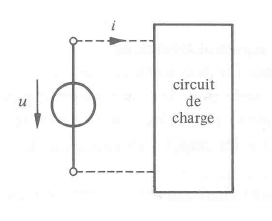
\includegraphics[scale=0.65]{images/source_tension}
		\caption{Une source de \textbf{tension} ``parfaite''}
		\label{subfig: source de tension}
	\end{subfigure}
	\begin{subfigure}[b]{0.27\textwidth}
		\captionsetup{justification=centering}	
		\centering
		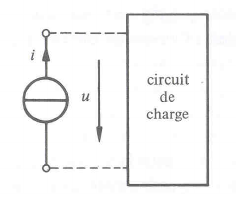
\includegraphics[scale=0.65]{images/source_courant}
		\caption{Une source de \textbf{courant} ``parfaite''}
		\label{subfig: source de courant}
	\end{subfigure}
	\begin{subfigure}[b]{0.27\textwidth}
		\captionsetup{justification=centering}	
		\centering
		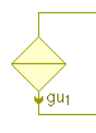
\includegraphics[scale=0.65]{images/source_commandee}
		\caption{Une source de courant commandée}
		\label{subfig: source de courant commandee}
	\end{subfigure}\\
	\begin{subfigure}[b]{0.45\textwidth}
		\centering
		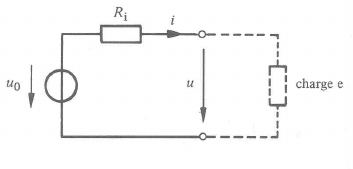
\includegraphics[scale=0.7]{images/tension_reelle}
		\caption{Représentation réelle d'une source de tension}
		\label{subfig: source tension reelle}
	\end{subfigure}
	\begin{subfigure}[b]{0.45\textwidth}
		\centering
		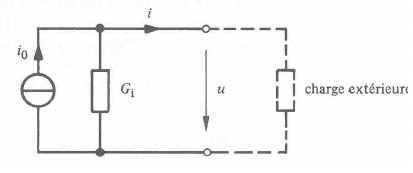
\includegraphics[scale=0.7]{images/courant_reelle}
		\caption{Représentation réelle d'une source de courant}
		\label{subfig: source courant reelle}
	\end{subfigure}	
	\caption{Représentation de différentes sources}
\end{figure}
De manière opposée, une source de courant est capable de fournir ou absorber de l'énergie électrique et dont \textit{le courant qui y circule} est constant et indépendant de la charge qui lui est branchée. Une source de courant ne peut fournir aucune énergie lorsqu'elle est \textit{branchée à un court-circuit}. Une telle source se représente comme à la figure  \ref{subfig: source de courant}.

\evid{Source réelle/idéale :} Similairement aux sources de tension, une source de courant devrait être totalement indépendante de la charge qui lui est branchée (comme représenté à la figure \ref{subfig: source de courant}) ; mais aussi comme pour les sources de tension, cela n'est pas vrai. Afin de mieux représenter le modèle, une source de courant est toujours représentée avec une résistance branchée en parallèle. De même, une représentation d'une source réelle se trouve à la figure \ref{subfig: source courant reelle}. Finalement, un calcul direct nous montre que 
\begin{equation}
	i = i_0 - G_iu
	\label{equ: resistance interne courant}
\end{equation}

\evid{Annulation :} Nous parlons parfois d'\textit{annuler une source de courant}. Cela consiste à la remplacer par un \textbf{circuit ouvert}.

\subsubsection{Sources commandées}
\label{subsubsection: source commandee}
Il est possible qu'une source dépende d'une tension où d'un courant ailleurs dans le circuit. Dans le cas d'une source de courant dépendant d'un courant $I_1$ ailleurs dans le circuit, la valeur de cette source serait décrite comme ``$\alpha I_1$''. Ces sources sont généralement considérées comme des sources standard. Il faut cependant faire attention lors de la simplification de circuits de ne pas altérer la ``commande'' de la source. Les sources commandées se représentent de la même manière que les sources indépendantes, en remplaçant le cercle par un carré ; la Figure \ref{subfig: source de courant commandee} représente une source de courant commandée par une tension.

\subsection{Kirchhoff}
\begin{figure}
	\centering
	\begin{subfigure}[b]{0.45\textwidth}
		\centering
		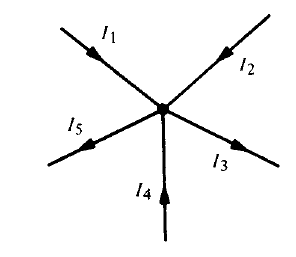
\includegraphics[scale=0.5]{images/kirchhoff_noeud}
		\caption{Un exemple de \textbf{n\oe ud}}
		\label{subfig: kirchhoff noeud}
	\end{subfigure}
	\begin{subfigure}[b]{0.45\textwidth}
		\centering
		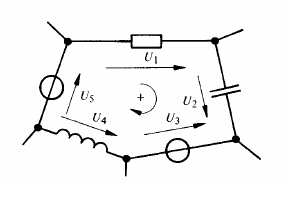
\includegraphics[scale=0.5]{images/kirchhoff_maille}
		\caption{Un exemple de \textbf{maille}}
		\label{subfig: kirchhoff maille}
	\end{subfigure}
	\caption{Application de la loi de Kirchhoff}
\end{figure}
Les lois de Kirchhoff représentent les bases de l'électricité moderne. Ces lois peuvent être utilisées de manières extrêmement diverses, mais sont toujours respectées pour tous les circuits. Ces lois se séparent en deux parties :

\begin{boite}
	\evid{Loi pour les n\oe uds :} Cette loi stipule que la somme des courants entrant et sortant d'un \uline{n\oe ud} est toujours exactement nulle. Pour un n\oe ud avec N branches connectées, cela se traduit simplement par la somme {suivante :}
	\begin{equation}
		\sum_{j=1}^N i_j = 0
	\end{equation}
\end{boite}
\begin{exemple}
	Appliquons cette formule sur le n\oe ud représenté à la Figure \ref{subfig: kirchhoff noeud}. La somme entre les courants entrants ($i_1,i_2, i_4$) et les courants sortants ($i_3, i_5$) doit être nulle, soit 
	\[i_1 + i_2 - i_3 + i_4 - i_5 = 0\]
\end{exemple}
\begin{boite}
	\evid{Loi pour les mailles :} Il est possible de définir une équation similaire pour les \uline{mailles}. En effet, cette loi stipule que (en choisissant un sens dans la maille, mais il n'importe pas), la somme des tensions aux bornes des éléments est nulle. Pour une maille à N éléments :
	\begin{equation}
		\sum_{j=1}^N u_j = 0
	\end{equation}
\end{boite}
\begin{exemple}
	Comme dans l'exemple précédent, nous allons appliquer cette formule à la maille visible à la figure \ref{subfig: kirchhoff maille}. Nous choisissons d'abord un sens (ici horaire) puis restons constant jusqu'à la fin de l'analyse. Dans ce sens, les tensions positives sont $U_1, U_2$ et $U_5$ alors que les négatives sont $U_3$ et $U_4$. Ainsi :
	\[U_1 +U_2 - U_3 - U_4 + U_5 = 0\]
\end{exemple}

\subsection{Mise en série}
\label{subsection: mise en serie}
\begin{figure}
	\centering
	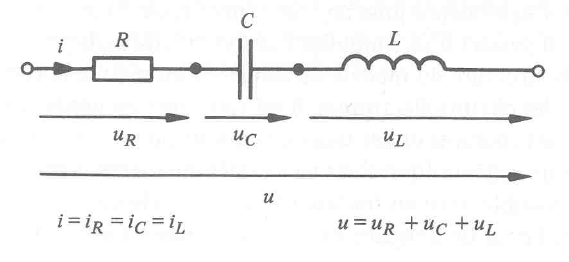
\includegraphics[scale=0.5]{images/mise_serie}
	\caption{Exemple d'éléments en série}
	\label{fig: mise en serie}
\end{figure}
\uline{Des éléments sont connectés en série s'ils sont parcourus par le même courant}, c'est à dire si un unique fil les traverse, sans séparation, comme à la Figure \ref{fig: mise en serie}. Notons que la tension aux bornes d'un tel circuit vaut la somme des tensions relatives à chaque élément. Également, l'ordre des éléments n'importe pas, nous considérons chaque type d'élément tour à tour ; avoir en série résistance -- inductance -- résistance -- inductance nous permet quand même d'appliquer la loi pour les résistances puis pour les inductances, et de mettre les éléments équivalents dans l'ordre souhaité.
\begin{boite}
	\evid{Résistances :} Pour obtenir la résistance équivalente, il suffit d'additionner la valeur des résistances. Pour $n$ résistances :
	\begin{equation}	
		R_{s} = \sum_{k=1}^n R_k
	\end{equation}
\end{boite}
\begin{boite}
	\evid{Capacités :} L'inverse du total est égal à la somme des inverses des capacités. Pour $n$ capacités :
	\begin{equation}
		\frac{1}{C_{s}} = \sum_{k=1}^n \frac{1}{C_k} \to \text{ (pour 2 capacités :) } C_{s} = \frac{C_1 \cdot C_2}{C_1 + C_2}
	\end{equation}		
\end{boite}
\begin{boite}
	\evid{Inductances :} Comme pour les résistances, la somme des inductances. Pour $n$ inductances :
	\begin{equation}
		L_{s} = \sum_{k=1}^n L_k	
	\end{equation}		
\end{boite}
\begin{boite}
	\evid{Sources de tension :} Encore pareil, la somme des sources (quelles qu'elles soient). Attention, dans le cas des sources, il est probable que certaines soient de sens différent. Dans ce cas, choisir un sens et considérer les sources dans ce sens comme positives, et celles dans le sens inverse comme négatives. Pour $n$ sources :
	\begin{equation}
		u_{s} = \sum_{k=1}^n u_k
	\end{equation}		
\end{boite}
\begin{boite}
	\evid{Sources de courant :} \textbf{IMPOSSIBLE}, sauf si toutes produisent le même courant. En effet, par Kirchhoff, tout courant qui rentre dans un point doit être le même que celui qui sort de ce point. En mettant une source de 2A suivie d'une source de 5A, cela signifierait que 2A rentrent dans la source de 5 et que 5A en sortent. 
\end{boite}
\subsection{Mise en parallèle}
\label{subsubsection: mise en parallele}
On dit de deux éléments qu'ils sont en parallèle s'ils partagent deux équipotentielles ---deux points points avec la même tension. Il est facile de voir (et donc de se rappeler) que les lois de mise en parallèle sont ``inverse'' par rapport à celles de la mise en série.
\begin{boite}
	\evid{Résistance :} L'inverse de la résistance équivalente vaut la somme de l'inverse des résistances. Pour $n$ résistances :
	\begin{equation}
		\frac{1}{R_p} = \sum_{k=1}^n \frac{1}{R_k}
	\end{equation}
\end{boite}
\begin{boite}
	\evid{Capacités :} La capacité équivalente vaut la somme des capacités. Pour $n$ capacités : 
	\begin{equation}
		C_p = \sum_{k=1}^n C_k
	\end{equation}
\end{boite}
\begin{boite}
	\evid{Inductances :} Comme pour les résistances, l'inverse de l'inductance équivalente vaut la somme de l'inverse des inductances. Pour $n$ inductances :
	\begin{equation}
		\frac{1}{L_p} = \sum_{k=1}^n \frac{1}{L_k}
	\end{equation}
\end{boite}
\begin{boite}
	\evid{Sources de tension :}  \textbf{IMPOSSIBLE}, sauf si les sources individuelles produisent la même tension. En effet, pour être en parallèle, les sources doivent partager une équipotentielle. Comme les sources produisent des tensions différentes, ces équipotentielles seraient à des potentiels différents, ce qui n'est par définition pas possible.
\end{boite}
\begin{boite}
	\evid{Source de courant :} Il suffit d'additionner les sources, dans leur sens respectif. Imaginez un circuit (au moins son dessin) dans lequel une source $I_1$ ``pointe vers le haut'' et une source $I_2$ ``pointe vers le bas'', alors il faudra calculer leur différence. 
	\begin{equation}
		i_{s} = \sum_{k=1}^n i_k
	\end{equation}
\end{boite}
\subsection{Exemple de réduction}
\label{Exemple: reduction de base}
\begin{figure}
	\centering
	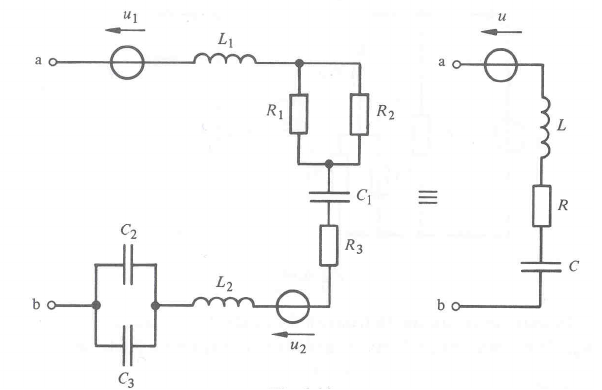
\includegraphics[scale=0.5]{images/exemple_combinaison_serie_parallele}
	\caption{Le circuit à réduire et sa réduction}
	\label{fig: exemple reduction serie/parallele}
\end{figure}
Nous allons analyser le circuit de gauche à la figure \ref{fig: exemple reduction serie/parallele}, afin de trouver son équivalent réduit (à droite). 

Commençons par les résistances : $R_1$ et $R_2$ sont en parallèle, et les deux sont en série avec $R_3$.
\[R = R_3 + \frac{1}{\frac{1}{R_1} + \frac{1}{R_2}} = R_3 + \frac{R_1R_2}{R_1+R_2}\]
Ensuite, comme les sources de courant sont en série, nous pouvons les additionner. $u_1$ est dans un sens, alors que $u_2$ est dans l'autre, donc nous calculons leur différence. Notons que retrancher $u_1$ à $u_2$ ou l'inverse n'a pas d'importance, car un considérer une tension de 5V dans un sens ou -5V dans l'autre est équivalent.
\[u = u_1 - u_2\]
Maintenant, les inductances sont en série, donc nous les additionnons simplement :
\[L = L_1 + L_2\]
Et enfin, la capacité 1 est en série avec les capacités 2 et 3, elles-même en parallèle entre elles. La réduction de la parallèle donne donc :
\[C_{23} = C_2 + C_3\]
Puis ajoutons la capacité 1 :
\[\frac{1}{C} = \frac{1}{C_1} + \frac{1}{C_{23}} = \frac{C_1 + C_{23}}{C_1\cdot C_{23}} \iff C = \frac{C_1C_{23}}{C_1 + C_{23}} = \frac{C_1(C_2 + C_3)}{C_++C_2+C_3}\]
Tous ces éléments se trouvant alors en série, nous trouvons le circuit de droite de la figure \ref{fig: exemple reduction serie/parallele}

\subsection{Diviseur de tension/courant}
\label{subsection: diviseur courant/tension}
\begin{figure}
	\centering
	\begin{subfigure}[b]{0.3\textwidth}
		\centering
		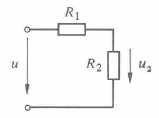
\includegraphics[scale=0.9]{images/diviseur_tension_r}
		\caption{}
		\label{subfig: diviseur tension R}
	\end{subfigure}
	\begin{subfigure}[b]{0.3\textwidth}
		\centering
		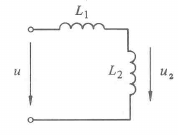
\includegraphics[scale=0.8]{images/diviseur_tension_l}
		\caption{}
		\label{subfig: diviseur tension L}
	\end{subfigure}
	\begin{subfigure}[b]{0.3\textwidth}
		\centering
		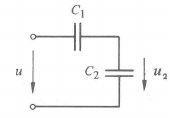
\includegraphics[scale=0.95]{images/diviseur_tension_c}
		\caption{}
		\label{subfig: diviseur tension C}
	\end{subfigure}\\
	\begin{subfigure}[b]{0.3\textwidth}
		\centering
		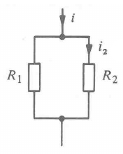
\includegraphics[scale=0.8]{images/diviseur_courant_r}
		\caption{}
		\label{subfig: diviseur courant R}
	\end{subfigure}
		\begin{subfigure}[b]{0.3\textwidth}
		\centering
		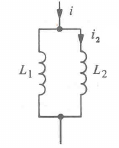
\includegraphics[scale=0.8]{images/diviseur_courant_l}
		\caption{}
		\label{subfig: diviseur courant L}
	\end{subfigure}
		\begin{subfigure}[b]{0.3\textwidth}
		\centering
		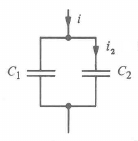
\includegraphics[scale=0.8]{images/diviseur_courant_c}
		\caption{}
		\label{subfig: diviseur courant C}
	\end{subfigure}
	\caption{Diviseur de \textbf{tension} (\textit{a} -- \textit{c}) et de \textbf{courant} (\textit{d} -- \textit{f})}
	\label{figs: diviseur tension courant}
\end{figure}
\evid{Tension :} Lorsque deux éléments passifs sont en série, la tension aux bornes d'un des deux éléments est une fraction (qui dépend de la valeur des deux éléments) de la tension totale. La règle générale pour cette fraction : \uline{la valeur \textit{vue} divisée par la valeur \textit{traversée totale}}. Dans les cas de la figure \ref{figs: diviseur tension courant} nous avons :
\begin{boite}
	\begin{equation}
		\ref{subfig: diviseur tension R}:\ u_2 = u\frac{R_2}{R_1 + R_2} \quad \ref{subfig: diviseur tension L} :\ u_2 = u\frac{L_2}{L_1 + L_2} \quad \ref{subfig: diviseur tension C} :\ u_2 = u\frac{C_2}{C_1 + C_2}
	\end{equation}
\end{boite}
Attention, pour le calcul du diviseur pour les capacités, il faut que les tension initiales soient nulles.\\
\\
\evid{Courant}
Pour appliquer le diviseur de courant, il faut que deux éléments de nature identique soient en parallèle. La règle est un peu différente ; la fraction se détermine avec : \uline{la valeur \textit{restante} divisée par la valeur \textit{traversée totale}}. De nouveau, dans les cas de la figure \ref{figs: diviseur tension courant} :
\begin{boite}
	\begin{equation}
		\ref{subfig: diviseur courant R}:\ i_2 = i\frac{R_1}{R_1 + R_2} \quad \ref{subfig: diviseur courant L} :\ i_2 = i\frac{L_1}{L_1 + L_2} \quad \ref{subfig: diviseur courant C} :\ i_2 = i\frac{C_1}{C_1 + C_2}
	\end{equation}
\end{boite}

\section{Méthodes d'Analyse}
\label{section: methode analyse}
\setcounter{equation}{0}
\subsection{Analyse nodale}
\label{subsection: analyse nodale}
Il s'agit d'une procédure générale d'analyse des circuits, dans laquelle nous utilisons \textit{les tensions des n\oe uds} comme variables du circuit. Cette analyse nous permettra de trouver les tensions des n\oe uds. Pour commencer, nous allons appliquer cette méthode à un circuit résistif à $n$ n\oe uds et sans source de tension. La marche à suivre est la suivante :
\begin{boite}
	\textbf{Analyse Nodale (théorie)}
	\begin{enumerate}
		\item 	Sélectionner le n\oe ud $n$ comme n\oe ud de référence. Attribuer les tensions $v_1,v_2$,\ldots,$v_{n-1}$ aux ($n-1$) autres n\oe uds. Les différences de potentiel sont établies par rapport au n\oe ud de référence.
		\item 	Appliquer la loi de Kirchhoff (pour les courants) à chacun des $n-1$ n\oe uds. Exprimer les courants des branches.
		\item 	Résoudre le système d'équations simultanées afin d’obtenir les valeurs des tensions inconnues.
	\end{enumerate}
\end{boite}

\subsubsection{Exemple d'application}
\label{exemple: application analyse nodale}
Nous partons avec le circuit de la figure \ref{subfig: nodale1}. La première étape, comme énoncé, consiste à placer un n\oe ud de référence (que nous plaçons en bas), nommer les autres (respectivement 1 et 2), y associer les courants (toujours par rapport à la masse, la référence), qui sont alors $v_1$ et $v_2$. Faire tout cela nous permet d'obtenir le circuit de la figure \ref{subfig: nodale2}. 

Pour la seconde étape : nous appliquons Kirchhoff aux n\oe uds : du n\oe ud 1 rentre un courant ($I_1$) et en sortent 3 $(I_2, i_1, i_2)$. Pour le n\oe ud 2, les courants rentrants sont $I_2$ et $i_2$ alors que le sortant est $i_3$. Le circuit de la figure \ref{subfig: nodale3} en résulte. Il nous est maintenant possible de placer les équations suivantes :\\
Pour le n\oe ud 1 :
\[I_1 = I_2 + i_1 + i_2\]
Pour le n\oe ud 2 :
\[I_2 + i_2 = i_3\]
Relations-courants-tensions :
\[i_1 = \frac{v_1}{R_1} \quad i_2 = \frac{v_1-v_2}{R_2} \quad i_3 = \frac{v_2}{R_3}\]

Dernière étape : il faut résoudre ce système. Nous pouvons remplacer les valeurs de $i_1,i_2,i_3$ dans les équations des n\oe uds 1 et 2 pour obtenir :
\[I_1 = I_2 + \frac{v_1}{R_1} + \frac{v_1 - v_2 }{R_2} \qquad I_2 + \frac{v_1-v_2}{R_2} = \frac{v_2}{R_3}\]
Nous pouvons réécrire ces équations en terme de conductances :
\[I_1 = I_2 + G_1v_1 +G_2(v_1-v_2) \qquad I_2 + G_2(v_1-v_2) = G_3v_2\]
Qu'il devient possible de mettre sous forme matricielle :
\[\begin{bmatrix}
	G_1 + G_2 & -G_2\\
	-G_2 & G_2 + G_3
\end{bmatrix}
\begin{bmatrix}
v_1\\
v_2
\end{bmatrix}
=
\begin{bmatrix}
I_1 - I_2\\
I_2
\end{bmatrix}
\]
Qu'il est ensuite simple de résoudre par différents moyens, comme la méthode de substitution, la méthode d'élimination, la règle de Kramer ou une inversion de matrice.
\begin{figure}
	\centering
	\begin{subfigure}[b]{0.3\textwidth}
		\centering
		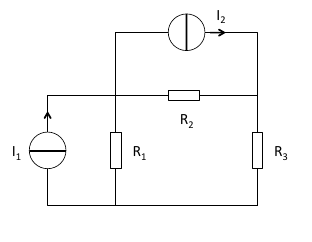
\includegraphics[scale=0.65]{images/nodale1}
		\caption{Le circuit à analyser}
		\label{subfig: nodale1}
	\end{subfigure}
	\begin{subfigure}[b]{0.3\textwidth}
		\centering
		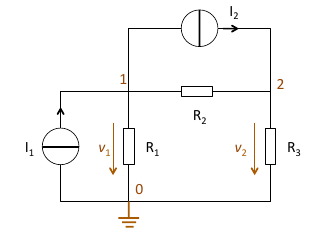
\includegraphics[scale=0.65]{images/nodale2}
		\caption{Placement des n\oe uds}
		\label{subfig: nodale2}
	\end{subfigure}
	\begin{subfigure}[b]{0.3\textwidth}
		\centering
		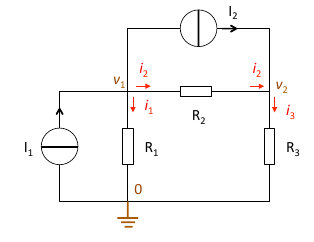
\includegraphics[scale=0.65]{images/nodale3}
		\caption{Après Kirchhoff}
		\label{subfig: nodale3}
	\end{subfigure}
	\caption{Les étapes 1 et 2 d'une analyse nodale}
	\label{figs: analyse nodale}
\end{figure}

\subsubsection[Rés. par inspection]{Résolution par inspection}
\label{subsubsection: nodale par inspection}
Regardons les matrices obtenues et notre circuit. Il est très facile de faire une liaison directe entre les deux : 
\begin{boite} 
	\textbf{Analyse nodale (par inspection)}
	
	Notre solution (encore à résoudre) est constituée d'un système composé d'une matrice G et de 2 vecteurs V et I\footnote{N'est pas la matrice identité} avec $m = n-1$, c'est à dire le nombre de n\oe uds du circuits moins 1\footnote{Car nous ``perdons'' un n\oe ud, le n\oe ud de référence} :
	\[G_{m\times m} \cdot V_{m} = I_{m}\]
	Les 3 matrices sont remplies ainsi :
	\begin{itemize}
		\item 	$G_{kk}$ (les éléments diagonaux) :la somme des conductances reliées au n\oe ud k.
		\item 	$G_{ij} = G_{ji}$ avec $i \neq j$ (les éléments non-diagonaux) : la somme (et signe négatif) des conductances reliant directement les n\oe uds $j$ et $j$.
		\item 	$V_{i}$ : les tensions $v_i$
		\item 	$I_{i}$ : les courants entrant (sortant $\to$ signe négatif) du n\oe ud $i$.
	\end{itemize}
\end{boite}
\subsubsection[Sources dépendantes]{Note sur les sources dépendantes}
\label{subsubsection: note sources dependantes}
\begin{figure}
	\centering
	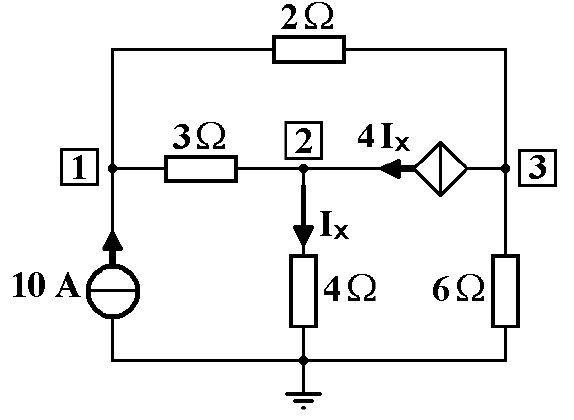
\includegraphics[scale=0.5]{images/nodale_source_dependante}
	\caption{Circuit avec une source dépendante}
	\label{fig: nodale source dependante}
\end{figure}
Il est possible qu'une analyse de circuit vous mette face à des sources dépendantes, comme c'est le cas à la figure \ref{fig: nodale source dependante}. Dans ce cas, comment les gérer ? Deux choix s'offrent à nous. Dans notre cas, nous pouvons mener une analyse sans la ``résolution par inspection'' ; nous regardons chaque n\oe ud et appliquons Kirchhoff en remplaçant les courant par des différences de tension. Par exemple, au n\oe ud 1 nous aurions :
\[10 = I_1 + I_2 = \frac{U_1-U_2}{3} + \frac{U_1-U_3}{2}\]
Mener une analyse similaire au n\oe ud 2 donne :
\[I_1 = -3I_x \iff \frac{U_1-U_2}{3} = -3\frac{U_2}{4}\]
Et finalement la même chose au n\oe ud 3 ; cela nous donne 3 équations avec 3 inconnues (résolution par exemple par matrices), et voilà.

Sinon, nous pouvons toujours mener notre résolution par inspection, mais en se rappelant de 2 choses : la définition de $I_x$ et la définition d'une matrice. Le remplissage de la matrice, comme nous savons le faire, nous donne :
\[\begin{bmatrix}
	\frac{1}{2} + \frac{1}{3} & -\frac{1}{3} & -\frac{1}{2} \\
	-\frac{1}{3} & \frac{1}{3} + \frac{1}{4} & 0\\
	-\frac{1}{2} & 0 &\frac{1}{2} + \frac{1}{6}
	\end{bmatrix}\begin{bmatrix}
	U_1\\
	U_2\\
	U_3
	\end{bmatrix} = \begin{bmatrix}
		10\\
		4 I_x\\
		-4I_x
	\end{bmatrix}\]
En simplifiant un peu :
\[\begin{bmatrix}
	\frac{5}{6} & -\frac{1}{3} & -\frac{1}{2} &\vline & 10\\
	-\frac{1}{3} & \frac{7}{12} & 0 & \vline & 4I_x\\
	-\frac{1}{2} & 0 & \frac{2}{3} & \vline & -4I_x
\end{bmatrix}\]
Maintenant, comme nous connaissons la définition de notre courant inconnu :
\[I_x = \frac{U_2}{4}\]
Nous nous rappelons qu'une matrice n'est rien d'autre qu'un système d'équations. Multiplier une ligne (donc une équation) par un scalaire ne changera pas la solution finale (c'est aussi vrai pour la méthode de Cramer). Nous pouvons donc remplacer $I_x$ par sa valeur et multiplier les lignes afin d'avoir des chiffres entiers :
\[\begin{bmatrix}
	5 & -2 & -3 & \vline & 60\\
	-4 & 7 & 0 & \vline & 12\cdot 4\frac{U_2}{4}\\
	-3 & 0 & 4 & \vline & -6 \cdot 4\frac{U_2}{4}
\end{bmatrix}\]
Mais si nous pensons maintenant en terme d'équations, la seconde ligne devient :
\[-4 U_1 + 7 U_2 = 12 U_2 \iff -4 U_1 - 5U_2 = 0 \iff 4U_1 + 5U_2 = 0\]
Et la troisième devient :
\[-3 U_1 + 4U_3 = -6 U_2 \iff -3U_1 + 6 U_2 + 4 U_3 = 0 \iff 3 U_1 - 6 U_2 - 4 U_3 = 0\]
Nous replaçons ces deux lignes dans notre matrice pour trouver :
\[\begin{bmatrix}
	5 & -2 & -3 & \vline & 60\\
	4 & 5 & 0 & \vline & 0\\
	3 & -6 & -4 & \vline & 0	
\end{bmatrix}\]
Pour finir, il suffit de résoudre ce système, par exemple avec la méthode de Cramer.

\subsection{Analyse de Mailles}
Maintenant que nous savons comment exécuter une analyse nodale pour trouver les tensions à chaque n\oe ud du circuit, nous pouvons trouver une méthode similaire en utilisant les \uline{courants des mailles} comme variables, afin de déterminer les courants inconnus. C'est la méthode complémentaire à la précédente : 
\begin{itemize}
	\item 	L'analyse nodale fait appel à la loi de Kirchhoff pour les \textit{courants} pour trouver les \textit{tensions inconnues}
	\item 	L'analyse de mailles utilise la loi de Kirchhoff pour les \textit{tensions} pour trouver les \textit{courants inconnus}
\end{itemize}
Attention cela dit, car cette méthode est moins générale car elle ne peut s'appliquer qu'aux circuits dont de type planaire.\\
\\
\evid{Note : qu'est-ce qu'un circuit de type planaire ?} Littéralement, il s'agit d'un circuit pour lesquels les branches ne se croisent pas.
\begin{figure}[!h]
	\centering
	\begin{subfigure}[b]{0.45\textwidth}
		\centering
		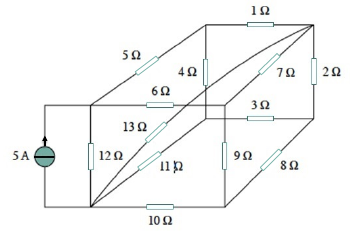
\includegraphics[scale=0.7]{images/non_planaire}
		\caption{Un circuit \textbf{non}-planaire}
		\label{subfig: non-planaire}
	\end{subfigure}
	\begin{subfigure}[b]{0.45\textwidth}
		\centering
		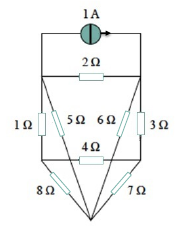
\includegraphics[scale=0.75]{images/planaire}
		\caption{Un circuit \textbf{planaire}}
		\label{subfig: planaire}
	\end{subfigure}
	\caption{Différence entre un circuit non planaire (ou spatial) et un planaire }
\end{figure}
Le circuit \ref{subfig: non-planaire} n'est clairement pas planaire ; en revanche, même si le circuit \ref{subfig: planaire} ne semble pas l'être, il est bien planaire. En effet, il suffit de redessiner les branches qui passent à l'intérieure pour les faire passer à l'extérieur sans altérer le circuit pour autant. Ce circuit est donc bien planaire.\\
\\
\evid{Note : qu'est-ce qu'une boucle ?} Nous allons pour cette méthode travailler dans les boucles d'un circuit, il est donc important de comprendre ce qu'est une boucle. Strictement parlant, une boucle est une maille qui ne contient pas d'autre maille en son sein.
\begin{figure}[!h]
	\centering
	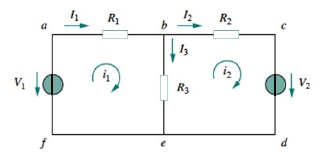
\includegraphics[scale=0.7]{images/maille_2_boucles}
	\caption{Exemple de maille à 2 boucles}
	\label{fig: maille 2 boucles}
\end{figure}
Par exemple, la figure \ref{fig: maille 2 boucles} est composée de 2 \textit{boucles} (chacun des deux rectangle) ; ce sont également des mailles. Et le grand rectangle, formé des deux plus petits est \uline{aussi} une maille. Mais comme elle contient d'autres mailles en son sein, ce n'est pas une boucle. Nous pouvons donc définir, pour notre figure, $i_1$ et $i_2$ qui sont les courants de boucle (et donc aussi de maille) pour chacune de ces petites boucles.\\
\\
\evid{La méthode :} Celle-ci se fait en trois étapes. Nous allons les appuyer avec un circuit d'exemple, celui de la figure \ref{fig: maille 2 boucles}.
\begin{enumerate}
	\item 	Identification des courants de maille : nous décidons des courants $i_1$ et $i_2$ (et de leur sens), et nommons les courants $I_1$, $I_2$,\ldots s'ils ne sont pas donnés.
	\item	Application de la loi de Kirchhoff (tensions). Pour notre exemple : \\ Maille 1 : \[-V_1 + R_1i_1 + R_3(i_1-i_2) = 0 \quad \text{ou} \quad (R_1 + R_3) i_1 - R_2i_2 = V_1\] Maille 2 : \[R_2i_2 + V_2 + R_3(i_2-i_1) = 0 \quad \text{ou} \quad -R_3i_1 + (R_2+R_3) i_2 = -V_2\]
	\item 	Résolution des équations. Nous n'avons qu'à mettre sous forme matricielle :
			\begin{equation}
				\begin{bmatrix}
					R_1 + R_3 & -R_3\\
					-R_3 & R_2 + R_3
				\end{bmatrix}
				\begin{bmatrix}
					i_1\\
					i_2
				\end{bmatrix} 
				=
				\begin{bmatrix}
					V_1\\
					-V_2
				\end{bmatrix}
				\label{equ: matrice analyse mailles}
			\end{equation}
		Et résoudre comme nous savons le faire.
\end{enumerate}

\subsubsection{Résolution par inspection}
Nous pouvons généraliser les matrices obtenues à l'équation \ref{equ: matrice analyse mailles} : notre système doit être de la forme 
\[R_{m\times m} \cdot I_{m} = V_m\]
Et en comparant avec notre précédent exemple, nous comprenons vite que le remplissage doit se faire ainsi :
\begin{boite}
	\begin{itemize}
		\item 	$R_{kk}$ : la somme des résistances appartenant à la maille $k$
		\item 	$R_{ij} = R_{ji}$ lorsque $i \neq j$ : somme (avec signe négatif) des résistances communes aux mailles $i$ et $j$.
		\item 	$I_k$ : le courant inconnu de la maille $i_k$
		\item 	$V_k$ : la somme des sources indépendantes de tension (dans le sens du courant de maille\footnote{Rappelons-nous que dans une source, la tension et le courant sont de sens inverse} ; c'est pour ça que nous avons $V_1$ et $-V_2$ dans notre exemple).
	\end{itemize}
\end{boite}
Ainsi, pour un circuit à $N$ mailles nous aurons un système de taille 
\[R_{N\times N} \cdot I_{N} = V_{N}\]

\subsubsection[Note sur les sources dépendantes]{Sources dépendantes}
Nous appliquons la même logique qu'au chapitre \ref{subsubsection: note sources dependantes}.
\section{Théorèmes fondamentaux}
\label{section: theo fondamentaux}
\evid{Circuit linéaire :} Un circuit est linéaire si sa sortie est reliée linéairement à son entrée ; de la même manière, il ne comporte que des éléments linéaires et des sources linéaires (dépendantes et indépendantes). 

\subsection{Principe de superposition}
Ce théorème dit que : ``le courant et les tensions dans un élément quelconque d'un circuit linéaire sont donnés par la somme des tensions et des courants produits dans cet élément par chaque source prise séparément''. 

Autrement dit, si nous voulons analyser un circuit avec une source de courant et une source de tension, nous pouvons (et il est souvent plus simple) de considérer deux circuits, un avec uniquement la source de tension et un uniquement avec la source de courant, calculer les tensions/courants partout puis superposer ces circuits et additionner les courants/tensions. 

Par exemple, si un circuit nous dit que le courant passant dans une résistance est de 2A et que l'autre dit qu'il est de 5A, alors en superposant nous trouvons que le courant réel passant dans cette résistance est de $2+5 = 7$A.

\uline{Attention cela dit !} Ce théorème ne s'applique pas à la puissance.

\subsection{Équivalence de sources}
Il peut-être encombrant de se trouver avec de multiples sources de courant et de tension, et ne pas pouvoir les regrouper. Nous pouvons le faire, en appliquant cette équivalence. Nous pouvons facilement prouver l'équivalence suivante : 
\begin{boite}
	Une source de tension en série avec une résistance équivaut à une source de courant en parallèle avec une résistance identique.
\end{boite}
\begin{exemple}
	une source de tension $u_0$ en série avec une résistance $R$ peut se transformer en une résistance $R$ en parallèle avec une source de tension $i_0 = \frac{u_0}{R}$. L'inverse est tout aussi vrai ($i_0$ en parallèle avec $R$ équivaut à $R$ en série avec $u_0 = R\cdot i_0$)
	\begin{center}
		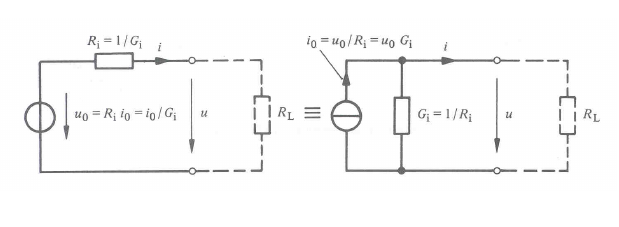
\includegraphics[scale=0.73]{images/equivalence_source}
	\end{center}
\end{exemple} 
Ce théorème est très pratique pour la réduction de circuits. En effet, une source de courant en parallèle avec une résistance, les deux en série avec une autre résistance ne peut pas se simplifier facilement ; mais en remplaçant les deux premiers en une source de tension en série avec la résistance, les deux résistances se trouvent en série et nous pouvons aisément les fusionner.

\subsection{Substitution de sources}
\begin{figure}[!h]
	\centering
	\begin{subfigure}[b]{0.45\textwidth}
		\centering
		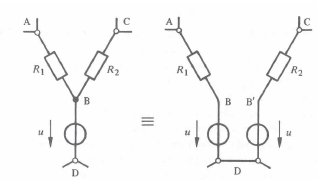
\includegraphics[scale=0.6]{images/substitution_tension}
		\caption{Sources de tension}
	\end{subfigure}
	\begin{subfigure}[b]{0.45\textwidth}
		\centering
		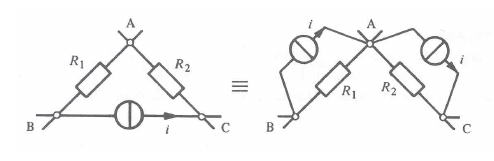
\includegraphics[scale=0.6]{images/substitution_courant}
		\caption{Sources de courant}
	\end{subfigure}
	\caption{Principe de substitution de sources}
\end{figure}

\subsection{Théorèmes de Thévenin et Norton}
\subsubsection{Théorème de Thévenin}
Le but de ce théorème est de remplacer tout circuit complexe (\textit{linéaire}) par un circuit composé d'une source de \textit{tension} et une résistance \textit{en série}, appelé son ``équivalent Thévenin''. Pour ce faire, nous appliquons la procédure suivante :
\begin{boite}
	\begin{itemize}
		\item 	Identifier les bornes du circuit et la charge externe
		\item 	Mesurer ou calculer la tension aux bornes du circuit sans charge extérieure ; c'est la \textit{tension de Thévenin}.
		\item 	Annuler les sources indépendantes\footnote{Pour savoir comment annuler une source : chapitres \ref{subsubsection: def source tension} et 	\ref{subsubsection: def source courant}} et déterminer la résistance vue des bornes du circuit ; c'est la \textit{résistance de Thévenin}.
	\end{itemize}
\end{boite}

\subsubsection{Théorème de Norton}
Il s'agit du corollaire au théorème de Thévenin. Le but est de remplacer un circuit complexe (\textit{linéaire}) par un circuit composé d'une source de \textit{courant} et une résistance \textit{en parallèle}, appelé son ``équivalent Norton''. La procédure est la suivante :
\begin{itemize}
	\item 	Identifier les bornes du circuit et la charge externe.
	\item 	Court-circuiter les bornes du circuit et déterminer théoriquement ou expérimentalement l'intensité du courant de court-circuit. C'est la \textit{source de courant de Norton}.
	\item 	Annuler les sources indépendantes et déterminer la résistance vue des bornes du circuit. C'est la \textit{résistance de Norton} (et de Thévenin, car il s'agit de la même).
\end{itemize}
\subsubsection{Transfert maximal de puissance}
Une des applications du théorème de Thévenin est le transfert maximal de puissance. 
\begin{figure}[!h]
	\centering
	\begin{subfigure}[b]{0.45\textwidth}
		\centering
		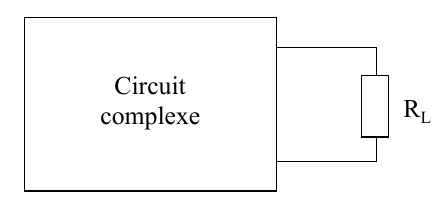
\includegraphics[scale=0.5]{images/transfert_max_puissance}
		\caption{Le dipôle et la résistance de charge}
		\label{subfig: transfert max puissance}
	\end{subfigure}
	\begin{subfigure}[b]{0.45\textwidth}
		\centering
		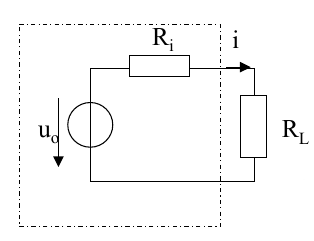
\includegraphics[scale=0.5]{images/thevenin_tmp}
		\caption{L'équivalent Thévenin du dipôle}
		\label{subfig: equi thevenin TMP}
	\end{subfigure}
	\caption{La résistance de charge, le dipôle complexe et son équivalent Thévenin}
\end{figure}
Nous avons un circuit complexe (que nous assimilons à un dipôle) connecté à une résistance de charge, comme visible à la figure \ref{subfig: transfert max puissance}. Quelle est la valeur de la résistance de charge pour que celle-ci dissipe un maximum de puissance ? Dans ce cas, nous devons remplacer le circuit complexe par son équivalent Thévenin (comme visible à la figure \ref{subfig: equi thevenin TMP}), et faire le raisonnement suivant : La puissance dissipée dans la résistance de charge vaut 
\[P = R_Li^2\]
Or, par 

\section{Régime sinusoïdal}
\label{sect: regime sinus}
\setcounter{equation}{0}
Le régime sinusoïdal est essentiel dans le cadre des circuits électriques. Nous allons donc, entre autres, aborder les concepts des fonctions périodiques en général, l'importance de ce régime, et analyser la réponse d'un circuit linéaire à une excitation sinusoïdale.

\subsection{Un peu de théorie}
\label{subsection: un peu de theorie}
Les définitions qui suivent sont valables pour toutes les fonctions $T$-périodiques.

Une \evid{fonction périodique} est une fonction qui vérifie la relation
\[f(t) = f(t+ nT)\]
pour tout $t$, où $n$ est un nombre entier et $T$ est \uline{la période}, qui correspond au temps pour compléter un cycle.

La \evid{valeur crête} (ou \textbf{l'amplitude}) A est la valeur maximale d'une fonction périodique.

La \evid{valeur crête à crête} correspond à l'écart maximal d'amplitudes atteint durant une période, c'est à dire la différence entre la valeur maximale et la valeur minimale.

La \evid{valeur moyenne $\overline{X}$} correspond, comme son nom l'indique, à un moyenne de la fonction durant un temps $t$. Elle se calcule ainsi :
\begin{equation}
	\overline{X} = \frac{1}{T}\int_t^{t+T} x(\tau) \deriv{\tau}	
	\label{equ: valeur moyenne}
\end{equation}

La \evid{valeur efficace} ---en anglais rms (Root Mean Square) value--- d'un courant (ou une tension) alternatif, correspond à la valeur d'un courant continu (ou d'une tension continue) qui produirait un échauffement identique dans une résistance. Celle-ci se calcule ainsi :
\begin{equation}
	X = \sqrt{\frac{1}{T}\int_t^{t+T} x^2(\tau) \deriv{\tau}}
\end{equation} 
Comme cette équation prend le carré de la fonction, il est important de noter que \uline{la valeur efficace est toujours positive}.

La \evid{fréquence} est l'inverse de la période et correspond au nombre de cycles par unités de temps. l'unité de la fréquence est le \textbf{hertz [Hz]}, qui est défini comme ``la fréquence d'un phénomène périodique dont la période T est une seconde''
\subsubsection{Quelques analyses}
Nous allons étudier les fonctions de type \textit{sinusoïdal}. Celles-ci ont certaines particularités ; par exemple toute partagent une forme commune, à savoir 
\begin{equation}
	x(t) = A\sinn{\frac{2\pi}{T}t + \alpha} = A\sin(2\pi ft + \alpha) = A\sin(\omega t + \alpha)
\end{equation}
Avec, comme précédemment, l'amplitude $A$, la période $T$, la fréquence $f$, la phase à l'origine $\alpha$ et {la pulsation} $\omega$. Cette forme générique se retrouve illustrée à la Figure \ref{fig: generique sinusoidal}
\begin{figure}
	\centering
	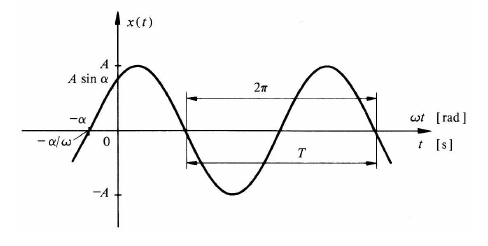
\includegraphics[scale=0.8]{images/sinusoidal}
	\caption{La forme commune d'une fonction sinusoïdale}
	\label{fig: generique sinusoidal}
\end{figure}

La \evid{pulsation} dont nous venons de parler, n'est autre que la fréquence angulaire, soit le nombre de rotations (du cercle trigonométrique) par seconde. Elle se mesure en $\left[\txtfrac{rad}{s}\right]$, avec la relation suivante :
\[\omega = 2\pi f = \frac{2\pi}{T}\]

Nos connaissances sur la valeur moyenne et la valeur efficace tiennent toujours, mais dans le cas précis des régimes sinusoïdaux, il devient plus facile de les calculer. Par exemple, comme nous avons affaire à une fonction parfaitement symétrique horizontalement, la valeur moyenne est toujours la même :
\[\overline{X} = 0 \]
Et la valeur efficace se calcule rapidement (preuve annexe \ref{app: preuves}) : 
\[X = \frac{A}{\sqrt{2}}\]

Maintenant que nous connaissons la valeur efficace, nous pouvons l'appliquer à la tension et au courant. Nous l'avons dit, le courant et la tension peuvent se définir ainsi :
\begin{equation}
	u(t) = \U \cos(\omega t + \alpha) \qquad i8t) = \I\cos(\omega t + \alpha)
\end{equation}
Nous avons juste à appliquer notre formule pour la valeur efficace :
\[U = \frac{\U}{\sqrt{2}} \qquad I = \frac{\I}{\sqrt{2}}\]
Ainsi, la valeur efficace de la tension et du courant en fonction du temps vaut :
\begin{equation}
	u(t) = \sqrt{2}U\cos(\omega t + \alpha) \qquad i(t) = \sqrt{2}I\cos(\omega t + \alpha)
	\label{equ: valeur efficace tension courant}
\end{equation}

\evid{Déphasage :} chaque sinusoïde possède une grandeur ``$\alpha$''  appelée la phase à l'origine. Nous définissons le déphasage entre deux grandeurs sinusoïdales ---par exemple entre la tension de phase $\alpha$ et le courant de phase $\beta$--- comme la différence des phases : 
\begin{equation}
	\varphi = \alpha - \beta
\end{equation}
Nous considérons toujours la valeur principale du déphasage comprise entre $-\pi \et \pi$. Si $\phi > 0$ alors la tension est en avance sur le courant. Sinon elle est en retard.

\subsubsection{Échauffement d'une résistance}
Comme nous le savons, la perte en énergie d'une résistance correspond à la puissance dissipée par celle-ci, caractérisée par le produit de la tension et du produit (en régime constant). Mais lorsque la tension (et le courant) est sinusoïdale, la puissance moyenne dissipée dans une résistance devient égale à l'intégrale, sur une période, de ce même produit. Mathématiquement, pour 
\[u(t) = \U \sin(\omega t) \et i(t) = \frac{\U}{R}\sin(\omega t)\]
La puissance en fonction du temps devient
\[p(t) = u(t)i(t) = Ri^2(t) = \frac{u^2(t)}{R} = \frac{\U^2}{R}\sin^2(\omega t)\]
Et l'échauffement :
\[P = \frac{1}{T}\int_0^T u(ti(t) \deriv{t} = \frac{1}{T}\frac{\U^2}{R}\int_0^T \sin^2(\omega t) \deriv{t} = \frac{\U^2}{2R}\]
Or, en utilisant ce que nous connaissant sur le courant et la tension (efficace), 
\[U = \frac{\U^2}{\sqrt{2}}  \qquad \left\{\begin{array}{l}
\U = R\I\\
I = \frac{\I}{\sqrt{2}}
\end{array}\right.\]
Nous pouvoir avoir des formes différentes et plus simples :	
\begin{boite}
	\begin{equation}
		P = \frac{U^2}{R} \quad \et \quad P = RI^2
	\end{equation}
\end{boite}
En fait ces résultats sont tout à fait cohérents. En effet, la valeur efficace a été définie (au chapitre \ref{subsection: un peu de theorie}) de sorte qu'un volt continu ou un volt alternatif produisent le même échauffement dans une résistance.
\subsubsection{Importance de ce régime}
Le régime sinusoïdal est essentiel dans la société moderne. En effet, la production d'énergie fournit une tension sinusoïdale car la conversion entre l'énergie mécanique et l'énergie électrique se fait grâceà la rotation d'un bobinage placé dans un champs électrique. 

De plus, la forme sinusoïdale est la seule fonction périodique qui possède une dérivée et une intégrale analogue (c.f le chapitre \ref{subsesction: phaseurs operations}).Également, la somme de deux fonctions sinusoïdales est toujours une fonction sinusoïdale.

 Finalement, nous pouvons représenter n'importe quelle fonction périodique $f(t)$ par des fonctions sinusoïdales ; c'est ce que nous appelons le développement en série de Fourier\footnote{Ce sujet ce sera pas développé dans ce cours, mais dans celui d'Analyse 3}. Que la fonction périodique soit un simple sinus redressé, une fonction .

\subsection{Les phaseurs}
\evid{Note :} Depuis ici, il devient primordial d'être à l'aise avec les nombres complexes. Un rappel succin se trouve à l'annexe \ref{app: rappel complexes}, page \pageref{app: rappel complexes}. 

\evid{Définition :} Par les nombres complexes, nous pouvons poser (valable pour la tension et le courant) que :
\begin{equation}
	x(t) = \sqrt{2}X \cos(\omega t + \theta) \iff \uline{x} = \sqrt{2}Xe^{j(\omega t + \theta)} = \sqrt{2}Xe^{j\theta}e^{j\omega t}
\end{equation}
Dans un circuit électrique linéaire en régime sinusoïdal permanent, tous les courants et les tensions ont la même pulsation $\omega$. Ainsi, dans l'équation ci-dessus, le terme $e^{j\omega t}$ est commun à toutes les grandeurs (les courants et les tensions du circuit). Toute grandeur peut donc être caractérisée uniquement par son amplitude (valeur efficace) $X$ et sa phase $\theta$. 
\begin{boite}[0.48]
\centering
	Le phaseur associé à x(t) : $\ux = Xe^{j\theta}$
\end{boite}
Il est important de comprendre qu'\textbf{un phaseur ne dépend pas du temps}

Nous pouvons faire l'analyse pour le courant et la tension, afin d'obtenir :
\begin{boite}
\begin{equation}
	\begin{array}{rcl}
	u(t) = U\sqrt{2}\cos(\omega t + \alpha) & \iff & \uu = Ue^{j\alpha}\\
	i(t) = I\sqrt{2}\cos(\omega t + \beta) & \iff & \uu = Ie^{j\beta}
	\end{array}
	\label{equ: relation courant tension phaseur}
\end{equation}
\end{boite}
\subsubsection{Opérations}
\label{subsesction: phaseurs operations}
Soient les phaseurs $\uu_k = U_ke^{j\alpha_k}$ (pour $k = 1,2)$ \textbf{de même fréquence $f$} (et donc de même pulsation $\omega$). Nous définissons les opérations de base :
\begin{boite}
	\evid{Addition :} 
	\begin{equation}
		\uu = \uu_1 + \uu_2 \to 
		\left\{\begin{array}{l}
			U = \sqrt{U_1^2 + U_2^2 + 2U_1U_2\cos(\alpha_1 - \alpha_2)}\\
			\alpha = \arctan\(\frac{U_1\sin(\alpha_1 + U_2\sin(\alpha_2)}{U_1\cos(\alpha_1) + U_2 \cos(\alpha_2)}\)
		\end{array}\right.
		\label{equ: phaseur addition}
	\end{equation}
\end{boite}

\begin{boite}
	\evid{Soustraction :}
	\begin{equation}
		\uu = \uu_1 + \uu_2 \to 
		\left\{
			\begin{array}{l}
				U = \sqrt{U_1^2 + U_2^2 - 2U_1U_2\cos(\alpha_1 - \alpha_2)}\\
				\alpha = \arctan\(\frac{U_1\sin(\alpha_1 - U_2\sin(\alpha_2)}{U_1\cos(\alpha_1) - U_2 \cos(\alpha_2)}\)
			\end{array}
		\right.
	\end{equation}
\end{boite}
Soient $\ux = Xe^{j\alpha},\ \uy = Ye^{j\beta}$, également \textbf{de même fréquence $f$ }. Alors :
\begin{boite}
	\evid{Multiplication :} 
	\begin{equation}
		\uz = \ux\cdot\uy =Xe^{j\alpha}Ye^{j\beta} = Ze^{j\phi} \qquad \text{avec } 
		\left\{\begin{array}{l}
			Z = X\cdot Y\\
			\phi = \alpha + \beta
		\end{array}\right.
	\end{equation}
\end{boite}

\begin{boite}
	\evid{Division :} 
	\begin{equation}
		\uz = \frac{\ux}{\uy} =\frac{Xe^{j\alpha}}{Ye^{j\beta}} = Ze^{j\phi} \qquad \text{avec } 
		\left\{\begin{array}{l}
			Z = \frac{X}{Y}\\
			\phi = \alpha - \beta
		\end{array}\right.
	\end{equation}
\end{boite} 
\begin{blackbox}
	Note : si nous voulons faire des opérations entre des phaseurs de fréquence différente, nous ne pouvons pas appliquer les formules ci-dessus. Il faut les transformer dans leur forme de valeur instantanée :
	\[Xe^{\alpha} \to X\sqrt{2}\cos(\omega t + \alpha)\]
	Puis simplement additionner ces valeurs
\end{blackbox}
Pour rappel, nous avons 
\begin{itemize}
	\item 	$x(t) = \sqrt{2}X\cos(\omega t + \theta)$, une \uline{grandeur sinusoïdale}. 
	\item 	$\uline{x} = Xe^{j\theta}e^{j\omega t}$ sa  \uline{valeur instantanée complexe}
	\item 	$\ux = Xe^{j\theta}$ le \uline{phaseur associé}. 
\end{itemize}
\begin{boite}
	\evid{Dérivation :} Nous cherchons la dérivation par rapport au temps : $y = \frac{\deriv{x}}{\deriv{t}}$ :
	\begin{equation}
		\uline{y} = \frac{\deriv{\uline{x}}}{\deriv{t}} = j\omega \uline{x} \iff \uy = j\omega \ux
	\end{equation}
	Donc, nous voyons que dériver une grandeur sinusoïdale équivaut à une multiplication par $j\omega$. Nous pouvons donc généraliser à la dérivée n-ième
	\begin{equation}
		\uz = \frac{d^n{\uline{x}}}{\deriv{t^n}} = (j\omega)^n \uline{x} \iff \uz = (j\omega)^n \ux
	\end{equation}
\end{boite}
\begin{boite}
	\evid{Intégration :} la formule pour la dérivation peut s'étendre à l'intégration. Nous cherchons $y = \int x(t) \deriv{t}$, l'intégration par rapport au temps.
	\begin{equation}
		\uy = \int \uline{x}\deriv{t} = \int Xe^{j\theta}e^{j\omega t} \deriv{t} = \frac{X}{j\omega}e^{j\theta}e^{j\omega t} = \frac{1}{j\omega}\uline{x} \iff \uy = \frac{1}{j\omega}\ux
	\end{equation}
\end{boite}
Ces dernières équations nous montre que l'utilisation d'une représentation complexe pour les grandeurs sinusoïdales permet de remplacer les opération de dérivation (respectivement d'intégration) par une simple multiplication (respectivement division) par $j\omega$. Cela permet de transformer des équations différentielles compliquées par de simples équations algébriques.
\begin{figure}
	\centering
	\begin{subfigure}[b]{0.45\textwidth}
		\centering
		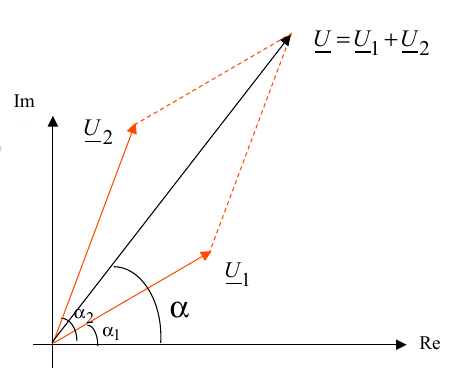
\includegraphics[scale=0.5]{images/phaseur_addition}
		\caption{L'addition}
	\end{subfigure}
	\begin{subfigure}[b]{0.45\textwidth}
		\centering
		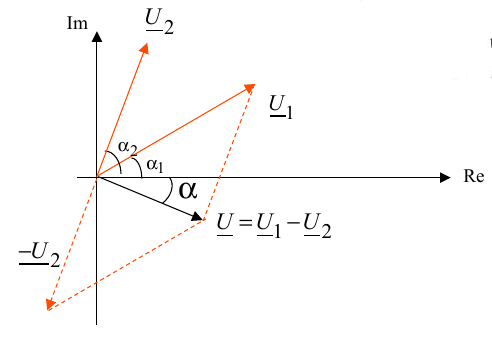
\includegraphics[scale=0.5]{images/phaseur_soustraction}
		\caption{La soustraction}
	\end{subfigure}
	\caption{Représentation des opérations de base sur les phaseurs}
\end{figure}

\subsection{Impédance et Admittance}
\textbf{Note :} jusqu'ici nous utilisions X,Y,Z comme des variables. Depuis maintenant et sauf mention contraire, $X,\ Y$ et $Z$ sont réservés, respectivement pour la réactance (c.f. plus loin), l'admittance et l'impédance.

Nous pouvons maintenant définir ce que sont l'impédance et l'admittance. Nous connaissons la tension $\uu = U e^{j\alpha}$ et le courant $\uline{I} = Ie^{j\beta}$.

\subsubsection{Impédance}
\label{subsubsection: def impedance}
\evid{L'impédance \uz} complexe d'un bipôle en régime permanent sinusoïdal, mesurée en \textbf{Ohm [$\ohm$]} peut être assimilée à la résistance, de par ses règles de calcul, mais en est très différente. Nous la définissons ainsi :
\begin{equation}
	\uz = \frac{\uline{u}}{\uline{i}} = \frac{\uu}{\uline{I}} = \frac{Ue^{j\alpha}}{Ie^{j\beta}} = Ze^{j\varphi} \qquad \text{avec } Z = \frac{U}{I} \et \varphi = \alpha-\beta
\end{equation}
En poussant le raisonnement plus loin, nous obtenons que :
\begin{equation}
	\uz = Ze^{j\varphi} = R + jX
\end{equation}
En utilisant les lois sur les nombres complexes (c.f. annexe \ref{app: rappel complexes}), nous voyons que 
\begin{equation}
	\left\{\begin{array}{ll}
		R = Z\cos\varphi & Z = \sqrt{R^2 + X^2}\\
		X = Z\sin\varphi & \varphi = \arctan\(\frac{X}{R}\)
	\end{array}\right.
\end{equation}
Nous notons toujours $R$ la \textbf{résistance} et $X$ la \textbf{réactance}.

\begin{figure}
	\centering
	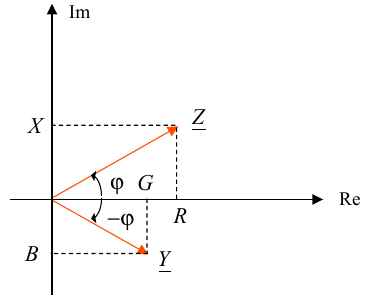
\includegraphics[scale=0.65]{images/imped_admit}
	\caption{Représentation graphique de l'impédance \uz et l'admittance \uy}
\end{figure}
\subsubsection{Admittance}
\label{subsubsection: def admittance}
\evid{L'admittance \uy} complexe d'un bipôle en régime permanent sinusoïdal se mesure en \textbf{Siemens [S]} et est l'inverse de l'impédance. 
\begin{equation}
	\uy =\frac{\uline{i}}{\uline{u}} = \frac{\uline{I}}{\uu} = \frac{1}{\uz} = \frac{Ie^{j\beta}}{Ue^{j\alpha}} = Ye^{-j\varphi} \qquad \text{avec } Y = \frac{I}{U} \et \varphi = \alpha-\beta
\end{equation}
Comme pour l'impédance, nous pouvons pousser le raisonnement :
\begin{equation}
	\uy =  Ye^{-j\varphi} = G + jB
\end{equation}
De même, en utilisons les lois sur les nombres complexes, nous pouvons voir que :
\begin{equation}
	\left\{\begin{array}{ll}
		G = Y\cos\varphi & Y = \sqrt{G^2 + B^2}\\
		B = -Y\sin\varphi & \varphi = \arctan\(-\frac{B}{G}\)
	\end{array}\right.
\end{equation}
En appelant $G$ la \textbf{conductance} et $B$ la \textbf{susceptance}
\subsubsection{Applications}
\label{subsubsection: impedance applications}
Ces concepts d'impédance et d'admittance sont extrêmement utiles une fois appliqués aux éléments de circuit que nous connaissons. Pour toutes les applications ci-dessous, nous utilisons toujours les même valeurs instantanées pour le courant et la tension, avec leur phaseur associé :
\begin{center}
	\begin{tabular}{l|r}
		valeur instantanée & phaseur\\
			\hline
		$u(t) = \sqrt{2}U\cos(\omega t + \alpha)$ & $\uu = Ue^{j\alpha}$\\
		$i(t) = \sqrt{2}U\cos(\omega t + \beta)$ & $\uline{I} = Ie^{j\beta}$\\
	\end{tabular}
\end{center}

\evid{Application à la résistance :}  nous avons vu précédemment la valeur instantanée $u(t) = Ri(t)$, ce qui nous donne immédiatement son phaseur ; 
\begin{boite}
	\begin{equation}
		\uu = R\uline{I}\Longrightarrow \uz_R = R, \quad Z_R = R, \quad \varphi_R = 0
		\label{equ: impedance resistance}
	\end{equation}
\end{boite}
\evid{Application à l'inductance :} même raisonnement : $u(t) = L\frac{\deriv{i}}{\deriv{t}} \to $
\begin{boite}
	\begin{equation}
		\uu = j\omega L\uline{I} \Longrightarrow \uz_L = j\omega L, \quad Z_L = \omega L, \quad \varphi_L = \pi/2
		\label{equ: impedance inductance}
	\end{equation}
\end{boite}
Plus précisément, selon la définition de l'impédance : $R_L = 0$ et $X_L = \omega L$\\
\evid{Application à la capacité :} idem :\[i(t) = C\frac{\deriv{u}}{\deriv{t}} \to \uline{I} = j\omega C \uu \iff \uu = \frac{1}{j\omega C} = -j\frac{1}{\omega C}\]
\begin{boite}
	\begin{equation}
		\Longrightarrow \uz_C = \frac{1}{j\omega C}, \quad Z_C = \frac{1}{\omega C},\ \varphi_C = -\pi/2
		\label{equ: impedance capacite}
	\end{equation}
\end{boite}
Comme pour l'inductance, nous avons plus précisément : $R_C = 0$ et $X_C = -\frac{1}{\omega C}$
\subsection{Exemple}
%dernière slide lecture 5
%TODO

\subsection{On recommence}
Nous avons analysé beaucoup de cas de circuits, et différentes lois que nous pouvons appliquer dessus. Nous avons vu comment réduire des circuits à d'autres plus simples afin de simplifier des calculs. Hé bien nous pouvons revisiter la plupart de ces concepts avec nos nouvelles connaissances sur l'impédance.

\evid{Source avec impédance interne :} Rappelons-nous la définition des sources (section \ref{subsubsection: def source tension} et \ref{subsubsection: def source courant}) ; nous y avons évoquer le concept de source idéale, mais auquel il ne fallait pas compter ; en revanche, un modèle plus réaliste comprenait une résistance interne (en série d'une source de tension et en série d'une source de courant). Il est possible de généraliser cette notion à celle \textbf{d'impédance interne}
\begin{figure}%[!h]
	\centering
	\captionsetup{justification=centering}
	\begin{subfigure}[b]{0.45\textwidth}
		\centering
		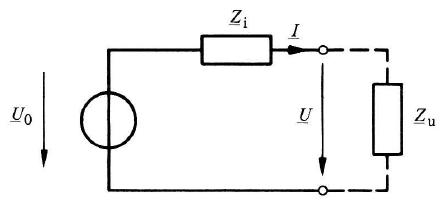
\includegraphics[scale=0.5]{images/source_tension_impedance}
		\caption{Impédance interne pour une source de tension}
	\end{subfigure}
	\begin{subfigure}[b]{0.45\textwidth}
		\centering
		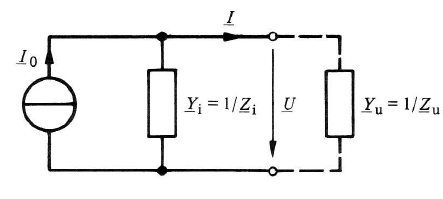
\includegraphics[scale=0.5]{images/source_courant_impedance}
		\caption{Impédance interne pour une source de courant}
	\end{subfigure}
	\caption{Généralisation de la notion de résistance interne : l'impédance interne}
	\label{figs: source impedance interne}
\end{figure}

Nous pouvons également reprendre les équations\footnote{Du chapitre \ref{section: notion de base}, page \pageref{equ: resistance interne courant}} \ref{equ: resistance interne tension} et \ref{equ: resistance interne courant} et les adapter avec l'impédance, afin d'obtenir les suivantes :
\[\uz_i = R_i + jX_i\qquad \uy_i = \frac{1}{\uz_i}\]
\begin{equation}	
	\uu = \uu_0 - \uz_i \, \uline{I} \qquad \uline{I} = \uline{I}_0 - \uy_i \, \uu
\end{equation}

\evid{Équivalence sources de tension/courant :} Il est également possible de reproduire l'équivalence entre une source de courant et une source de tension ; par exemple, les deux sources de la figure \ref{figs: source impedance interne} peuvent être inter-changées avec les règles suivantes :
\begin{equation}
	\uu_0 = \uz_i \, \uline{I}_0 \qquad \uline{I}_0 = \uy_i \uu_0 = \frac{\uu_0}{\uz_i}
\end{equation}

\evid{Mise en série d'impédances (admittances) :} Dans ce point et le suivant, nous voyons à quel point l'impédance (respectivement l'admittance) est proche de la résistance (respectivement la conductance) ; en effet, en plus des relations avec le courant et la tension, la mise en série (et en parallèle) est similaire :
\begin{equation}
	\uz_s = \sum_{k=1}^n \uz_k \qquad {Y}_s = \frac{1}{\uz_s} = \frac{1}{\somme{n}{k=1}\uz_k} =  \frac{1}{\somme{n}{k=1} \frac{1}{\uy_k}}
	\label{equ: mise serie impedance/admittance}
\end{equation}

\evid{Mise en parallèle d'impédances (admittances) :} Similairement :
\begin{equation}	
	\uy_p = \sum_{k=1}^n \uy_k \qquad {Z}_p = \frac{1}{\uy_p} = \frac{1}{\somme{n}{k=1}\uy_k} =  \frac{1}{\somme{n}{k=1} \frac{1}{\uz_k}}
	\label{equ: mise parallele impedance/admittance}
\end{equation}

\evid{Bipôles composites élémentaires}
%%%%%%%%%%%%
%%%%%Si besoin de mettre l'un au dessous de l'autre
%%%%%%%%%%%%%
%\begin{figure}[!h]
%	\centering
%	\begin{subfigure}[b]{0.9\textwidth}
%		\centering
%		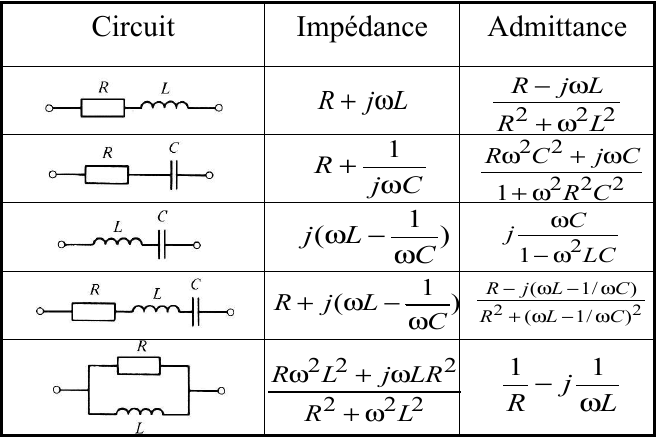
\includegraphics[width=7.5cm]{images/bipoles_impedance}
%	\end{subfigure}
%	~\\
%	\begin{subfigure}[b]{0.9\textwidth}
%		\centering
%		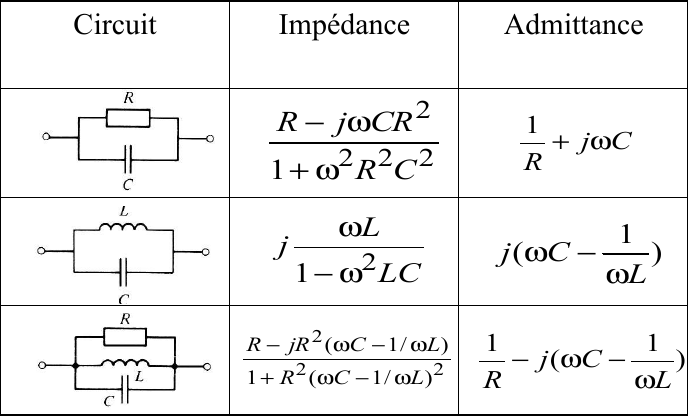
\includegraphics[width=7.5cm]{images/bipoles_impedance2}
%	\end{subfigure}
%\end{figure}
\begin{figure}[!h]
	\centering
	\begin{subfigure}[b]{0.45\textwidth}
		\centering
		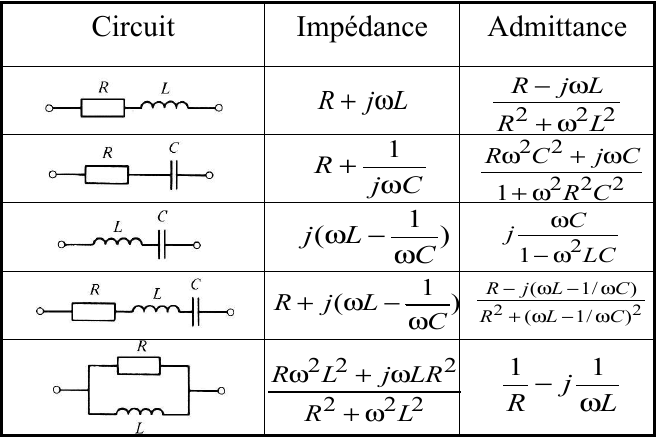
\includegraphics[height=4.5cm]{images/bipoles_impedance}
	\end{subfigure}
	\begin{subfigure}[b]{0.45\textwidth}
		\centering
		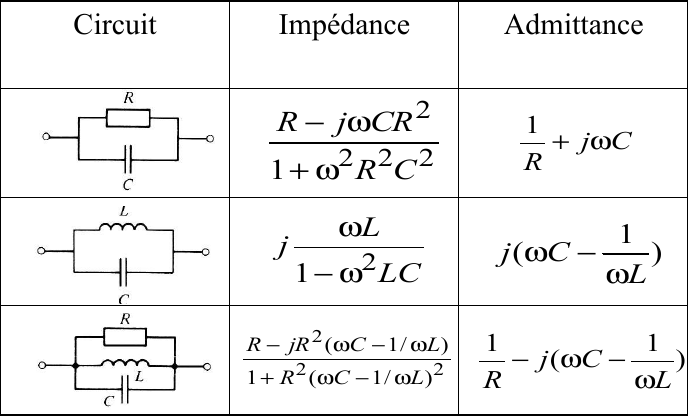
\includegraphics[height=4.5cm]{images/bipoles_impedance2}
	\end{subfigure}
	\caption{Résumé de quelques bipôles composites très simples}
	\label{figs: resume bipole composite}
\end{figure}
Nous voyons immédiatement que pour exprimer des circuits en série, utiliser l'impédance est bien plus simple, alors que l'admittance se révèle utile dans l'expression de circuits en parallèle. 
\begin{exemple}
	À titre d'exemple, tentons de retrouver l'expression de l'avant-dernier circuit, composé d'une inductance et une capacité en parallèle.
	
	\uline{Impédance :} Depuis le chapitre \ref{subsubsection: impedance applications}, nous connaissons l'impédance de l'inductance et de la capacité, respectivement :
	\[\uz_L = j\omega L \qquad \uz_C = \frac{1}{j\omega C}\]
	Nous venons aussi de voir la mise en parallèle d'impédances (equation \ref{equ: mise parallele impedance/admittance}). En combinant tout cela, nous obtenons 
	\begin{align*}
		\frac{1}{\uz_{tot}} = \frac{1}{\uz_L} + \frac{1}{\uz_C} = \frac{1}{j\omega L} + j\omega C \cdot \frac{j\omega L}{j\omega L} = \frac{1}{j\omega L} + \frac{j^2 \omega^2 CL}{j\omega L}\\
		 = \frac{1+j^2\omega CL}{j\omega L} = \frac{1-\omega^2 CL}{j\omega L} \to \uz_{tot} = j\frac{\omega L}{1-\omega^2 CL}
	\end{align*}
	
	\uline{Admittance :} Encore plus simple !
	\[\uy_{L} = \frac{1}{j\omega L} \qquad \uy_C = j\omega C \]
	Avec nos connaissances sur la mis en parallèle d'admittances :
	\begin{align*}
		\uy_{tot} = \uy_C + \uy_L = j\omega C + \frac{1}{j\omega C} = j\omega C - j\frac{1}{\omega L} = j\(\omega C - \frac{1}{\omega C}\)
	\end{align*}
\end{exemple}
\newpage
\evid{Tripôles équivalents :} Il peut être bon de savoir que les tripôles suivants sont équivalents, avec les règles associées :
\begin{figure}[!h]
	\centering
	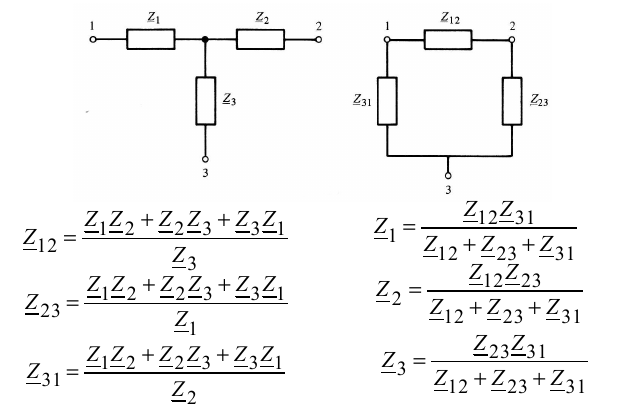
\includegraphics[scale=0.7]{images/tripoles}
	\caption{Deux tripôles équivalents}
	\label{fig: tripole equiv}
\end{figure}

\evid{Diviseurs de tension et de courant :} Comme vu précédemment, en ayant des résistances en série ou en parallèle, nous pouvons déterminer le courant ou la tension dans des parties en utilisant le concept de diviseur de tension ou de courant. Soient les circuits suivants :
\begin{figure}[!h]
	\centering
	\begin{subfigure}[b]{0.45\textwidth}
		\centering
		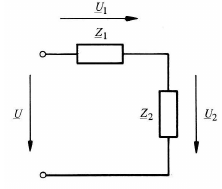
\includegraphics[scale=0.65]{images/diviseur_tension_impedance}
	\end{subfigure}
	\begin{subfigure}[b]{0.45\textwidth}
		\centering
		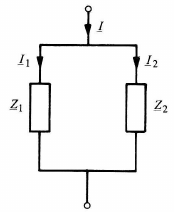
\includegraphics[scale=0.65]{images/diviseur_courant_impedance}
	\end{subfigure}
\end{figure}

Nous pouvons placer des équations similaires que pour les diviseurs standard, à savoir :
	\begin{align}
	\uu_1 = \frac{\uz_1}{\uz_1 + \uz_2}\uu \qquad \uu_2 = \frac{\uz_2}{\uz_1 + \uz_2}\uu\\
	\ui_1 = \frac{\uz_2}{\uz_1 + \uz_2}\ui \qquad \ui_2 = \frac{\uz_1}{\uz_1 + \uz_2}\ui
	\end{align}
\evid{Norton et Thévenin en régime sinusoïdal :} Toujours dans la même idée, nous pouvons appliquer Thévenin et Norton avec la notion d'impédance. \\

\uline{Thévenin:} Tout circuit peut être réduit à une source de \textit{tension} et une impédance en \textit{série}. Mathématiquement, et en considérant la figure \ref{fig: thevenin impedance} :
\begin{figure}[!h]
	\centering
	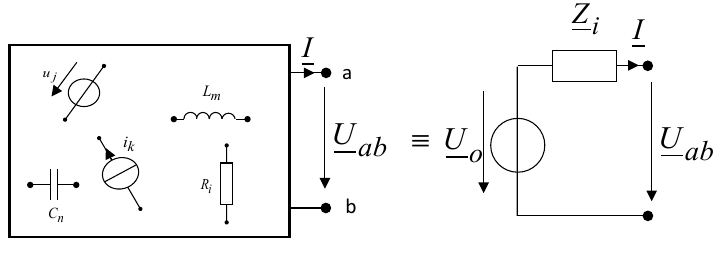
\includegraphics[scale=0.5]{images/thevenin_impedance}
	\caption{Équivalent Thévenin}
	\label{fig: thevenin impedance}
\end{figure}

\begin{equation}
	\uu_0 = \uu_{ab}\Big|_{\ui = 0} \qquad \uz_i = \uz_{ab}\Big|_{u_j = 0,\ i_k = 0}
\end{equation}

\uline{Norton :} Tout circuit peut être réduit à une source de \textit{courant} et une impédance en \textit{parallèle}. Mathématiquement, et en considérant la figure \ref{fig: norton impedance} :
\begin{figure}[!h]
	\centering
	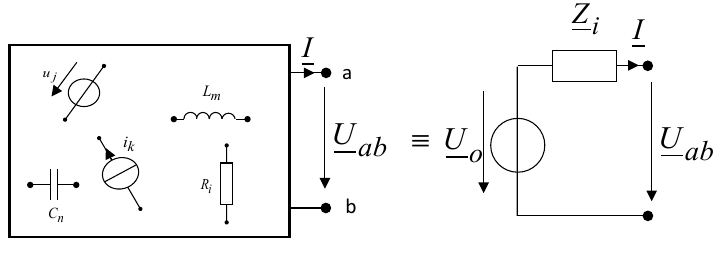
\includegraphics[scale=0.5]{images/thevenin_impedance}
	\caption{Équivalent Thévenin}
	\label{fig: norton impedance}
\end{figure}
\begin{equation}
	\uu_0 = \uu_{ab}\Big|_{\ui = 0} \qquad \uz_i = \uz_{ab}\Big|_{u_j = 0,\ i_k = 0}
\end{equation}


\subsection{Diagramme}
\subsubsection{D'impédance}
\begin{figure}
	\centering
		\begin{subfigure}[b]{0.32\textwidth}
		\centering
		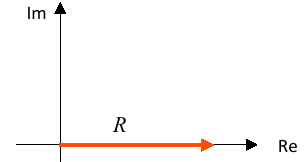
\includegraphics[scale=0.55]{images/diagramme_resistance}
		\caption{Pour une résistance R}
	\end{subfigure}
		\begin{subfigure}[b]{0.32\textwidth}
		\centering
		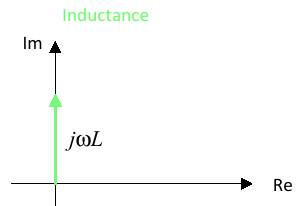
\includegraphics[scale=0.55]{images/diagramme_inductance}
		\caption{Pour une inductance L}
	\end{subfigure}
	\begin{subfigure}[b]{0.32\textwidth}
		\centering
		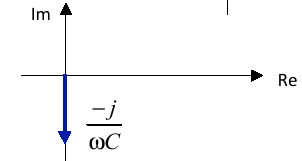
\includegraphics[scale=0.55]{images/diagramme_capacite}
		\caption{Pour une capacité C}
	\end{subfigure}
	\caption{Représentation d'impédances}
	\label{figs: representation impedance}
\end{figure}
Dans cette section, nous allons mettre en image les relations entre les impédances. Pour cela, nous dessinons un système d'axes, avec, en guise d'abscisse, l'axe Re (des réels) et en ordonnée l'axe Im (les imaginaires). Nous n'avons ensuite plus qu'à placer ensuite les impédances connues, à savoir la résistance ($R + j0$), l'inductance ($0 + j\omega L$) et la capacité ($0 -j\frac{1}{\omega C}$), pour obtenir les illustrations de la figure 	\ref{figs: representation impedance}. La composition de ces éléments se représente donc aisément.
\begin{exemple}
	Prenons un circuit RLC série (résistance, inductance et capacité en série), correspondant à la 4ème ligne du tableau de gauche à la figure \ref{figs: resume bipole composite}. En composant les règles vues ci-dessus, nous obtenons (en fonction du rapport entre C et L) une des deux solutions ci-dessous :
\end{exemple}
	\begin{figure}[!h]
		\centering
			\begin{subfigure}[b]{0.45\textwidth}
			\centering
			\includegraphics[scale=0.6]{images/impedance_petitL}
			\caption{Pour le cas $\omega L < \frac{1}{\omega C}$}
		\end{subfigure}
			\begin{subfigure}[b]{0.32\textwidth}
			\centering
			\includegraphics[scale=0.6]{images/impedance_grandL}
			\caption{Pour le cas $\omega L > \frac{1}{\omega C}$}
		\end{subfigure}
		\caption{Impédances dans un circuit RLC série}
	\end{figure}
\begin{center}
	\framecolorbox{white}{gray!20}{%
		\begin{minipage}{0.8\textwidth}
			Cela nous permet, par exemple, de comprendre la relation entre $\varphi$ et les parties réelle et imaginaire : une fois tous les ``vecteurs'' additionnés, nous avons une partie imaginaire (verticale) et une partie réelle (horizontale). La diagonale (la somme des deux parties) devient alors l'impédance \uz. C'est à cause de cela (et des règles élémentaires de trigonométrie) que nous avons la relation
			\[\tan(\varphi) = \txtfrac{partie imaginaire}{partie réelle}\]
		\end{minipage}
	}
\end{center}

\subsubsection{De phaseur}
Nous pouvons mener la même analyse, avec le même système d'axes, mais en considérant cette fois le courant et la tension. 
\begin{exemple}
	Prenons le même circuit que précédemment dans l'exemple précédent. Cette fois nous recevons le courant $\ui = Ie^{j\beta}$ et cherchons à calculer \uu. Par notre expérience, nous savons que :
	\[\uu_R = R\ui \qquad \uu_L = j\omega L\ui \qquad \uu_C = \frac{1}{j\omega C}\ui\]
	\[\uu = \uu_R + \uu_L + \uu_C\]
Comme nous l'avons appris, la composante $\beta$ est commune à tous les composants de ce circuit (vu qu'ils partagent le même courant). Nous avons donc simplement à reporter les grandeurs en suivant les axes, puis à pivoter l'ensemble d'un angle $\beta$. De plus, il devient facile de trouver $\alpha$ graphiquement (voir figure \ref{fig: vecteurs}).
\end{exemple}
\begin{figure}[!h]
	\centering
	\includegraphics[scale=0.7]{images/diagramme_phaseur}
	\caption{On reporte nos ``vecteurs'' sur le diagramme}
	\label{fig: vecteurs}
\end{figure}

\subsection{Pertes}
\label{subsection: phaseur pertes}
\subsubsection{Inductance}
\begin{figure}
	\centering
	\begin{subfigure}[b]{0.45\textwidth}
		\centering
		\includegraphics[scale=0.7]{images/inductance_serie}
		\caption{Modèle en série}
		\label{subfig: inductance_serie}
	\end{subfigure}
	\begin{subfigure}[b]{0.45\textwidth}
		\centering
		\includegraphics[scale=0.7]{images/inductance_parallele}
		\caption{Modèle en parallèle}
		\label{subfig: inductance_parallele}
	\end{subfigure}
\end{figure}
Une inductance réelle n'est pas parfaite, elle comporte des pertes ; il est possible d'adapter notre modèle en ajoutant une résistance $R_s$ en série avec notre inductance $L_s$ (figure \ref{subfig: inductance_serie}). Équivalemment, nous pouvons utiliser un modèle avec une série $R_p$ en parallèle avec notre inductance $L_p$ (figure \ref{subfig: inductance_parallele}). Nous pouvons alors définir \textbf{le facteur de qualité $Q$ de l'inductance}
\begin{equation}
	Q = \txtfrac{réactance}{résistance} = \frac{\omega L_s}{R_s} = \frac{R_p}{\omega L_p}
\end{equation}
Et, lorsque $Q^2$ est bien plus grand que 1 :
\begin{equation}
L_s = L_p\quad R_p = Q^2R_s
\end{equation}
La preuve se trouve dans l'annexe \ref{app: preuve facteur qualite inductance}.

\subsubsection{Capacité}
Nous pouvons poser le même constat et le même raisonnement pour la capacité. Le facteur de qualité est alors défini comme 
\begin{equation}
	Q = \txtfrac{réactance}{résistance série} = \frac{1/\omega C_s}{R_s} = \frac{R_p}{1/\omega R_p} = \txtfrac{résistance parallèle}{réactance}
\end{equation}
Et pour $Q >> 1$ :
\begin{equation}
	C_s = C_p \qquad R_p = Q^2 R_s
\end{equation}

\subsection{Circuit résonnant}
Maintenant que chaque élément a été remanié pour coller au mieux à la réalité, considérons le circuit de la figure \ref{subfig: circuit resonnant} ;
\begin{figure}
	\begin{subfigure}[b]{0.45\textwidth}
		\centering
		\includegraphics[scale=0.6]{images/circuit_resonnant}
		\caption{Un circuit basique}
		\label{subfig: circuit resonnant}
	\end{subfigure}
	\begin{subfigure}[b]{0.45\textwidth}
		\centering
		\includegraphics[scale=0.6]{images/circuit_resonnant_reduit}
		\caption{Sa version réduite}
	\end{subfigure}
	\caption{Un circuit dont nous considérons le modèle ``ajusté'' des éléments, avec des résistances}
\end{figure}
nous savons maintenant qu'il est correct de considérer les éléments de base avec une résistance en série (ou parfois en parallèle). Par les formules vues auparavant, nous calculons :
\begin{itemize}
	\item 	L'impédance 
			\[\uz = R + j\(\omega L - \frac{1}{\omega C}\)\]
	\item 	Le courant dans le circuit
			\[\ui = \frac{\uv}{\uz} = \frac{\uv}{R + j\(\omega L - \frac{1}{\omega C}\)}\]
	\item 	L'amplitude et la phase du courant (pour $\uz = a + jb$)
			\begin{align*}
				I = \frac{V}{Z} = \frac{V}{\sqrt{a^2 + b^2}} = \frac{V}{\sqrt{R^2 + \(\omega L - \frac{1}{\omega C}\)^2}}\\
				\phi = -\tan^{-1}\left[ \frac{b}{a} \right] = -\tan^{-1} \left[ \frac{\omega L - \frac{1}{\omega C}}{R} \right] 
			\end{align*} 
\end{itemize}
\begin{figure}
	\centering
	\includegraphics[scale=0.5]{images/nature_impedance}
	\caption{Graphe de la réactance en fonction de la pulsation}
	\label{fig: graph nature impedance}
\end{figure}
\evid{Analyse de la nature de l'impédance :} Nous reportons sur un graphe la réactance en fonction de $\omega$. Dans notre cas, nous obtenons le graphe de la figure \ref{fig: graph nature impedance}. Sur celui-ci, nous reportons avec la courbe verte $\omega L$ (donc linéaire, de pente L), et avec la courbe violette $-\frac{1}{\omega C}$ (fonction inverse négative). En additionnant ces deux, nous trouvons la courbe bleue, qui correspond à la réactance totale. Nous pouvons facilement identifier la valeur \uline{$\omega_0$}, qui se trouve lorsque la réactance est nulle. En fonction de la valeur de $\omega$, nous nous trouvons face à 3 possibilités :
\begin{itemize}
	\item 	$\omega < \omega_0$ : la réactance est négative, \textbf{l'impédance est de nature capacitive} (car la capacité l'emporte sur l'inductance).
	\item 	$\omega > \omega_0$ : la réactance est positive, \textbf{l'impédance est de nature inductive} (car l'inductance l'emporte sur la capacité).
	\item 	$\omega = \omega_0$ (ici $\omega_0 = \frac{1}{\sqrt{LC}}$). Dans ce cas, il n'y a pas de partie imaginaire donc le circuit se comporte comme une résistance pure ; \textbf{l'impédance est de nature résistive} ; le courant passe par une valeur maximale : $I_0 = \frac{V}{R}$
\end{itemize}

Ainsi, nous montrons simplement que 
\begin{equation}
	\omega_2 - \omega_1 = \frac{R}{L} = \omega_0 \frac{R}{\omega_0 L} = \frac{\omega_0}{Q_0}
\end{equation}
En rappelant que $f_0 = \frac{\omega_0}{2\pi}$, nous définissons \textbf{la bande passante du circuit} :
\begin{equation}
	B = \frac{f_0}{Q_0}
\end{equation}

\evid{Importance de ce facteur de qualité :} La dernière équation nous montre la relation entre la bande passante et le facteur de qualité. Plus le facteur de qualité est grand, plus la bande passante est petite (et vice-versa). La sélectivité en fréquence et les propriétés d'amplification de circuits résonnants jouent un grand rôle dans la télécommunication. Ces propriétés sont faciles à décrire grâce au facteur de qualité.
\begin{exemple}
	Lorsqu'un circuit résonnant est utilisé dans un récepteur radio pour sélectionner une station parmi d'autres, il est important d'utiliser un circuit avec un grand facteur de qualité pour éviter de recevoir ds signaux d'une station adjacente. Un exemple est visible à la figure ci-dessous :
\end{exemple}
\begin{figure}[!h]
	\centering
	\includegraphics[scale=0.55]{images/importance_facteur_qualite}
\end{figure}
\begin{suiteExemple}
	Nous voyons qu'avec un petit facteur de qualité (courbe violette), nous aurons une faible réponse du récepteur. En revanche, un trop grand Q n'est pas désirable non plus, car les composantes fréquentielles du signal seront atténuées.
	
	Mentionnons également que la situation dans la figure précédente est hautement simplifiée ; en pratique, plusieurs circuits résonnants sont utilisés dans un récepteur, chacun accordé à une fréquence légèrement différente pour atteindre la fréquence désirée.
\end{suiteExemple}
\subsection{Lieu complexe}
\begin{figure}
	\centering
	\begin{subfigure}[b]{0.45\textwidth}
		\centering
		\includegraphics[scale=0.5]{images/lieu_de_z}
		\caption{Lieu de $\textbf{\uz}$ d'un circuit \textit{série}}
		\label{subfig: lieu complexe de z}
	\end{subfigure}
	\begin{subfigure}[b]{0.45\textwidth}
		\centering
		\includegraphics[scale=0.55]{images/lieu_de_y}
		\caption{Lieu de $\textbf{\uy}$ d'un circuit \textit{parallèle}}
		\label{subfig: lieu complexe de y}
	\end{subfigure}\\
	\begin{subfigure}[c]{0.9\textwidth}
		\centering
		\includegraphics[scale=0.5]{images/lieu_de_z_para}
		\caption{Lieu de $\textbf{\uz}$ d'un circuit \textit{parallèle}}
		\label{subfig: lieu complexe de z para}
	\end{subfigure}
	\caption{Lieu complexe pour un circuit en série et un circuit en parallèle.}
\end{figure}Le lieu complexe relatif à une grandeur complexe est le lieu décrit par l'extrémité du vecteur représentant cette grandeur lorsqu'on fait varier un paramètre, généralement la pulsation $\omega$.

Pour analyser ceci, nous reprenons notre circuit RLC série, d'impédance $\uz = R + j(\omega L - \frac{1}{\omega C})$. Nous pouvons ainsi reporter le lieu de \uz dans le système d'axes Réels/Imaginaires, comme visible à la figure \ref{subfig: lieu complexe de z}. 

Si en revanche, nous considérons un circuit avec ces 3 même éléments en parallèle, nous obtenons un circuit d'admittance $\uy = \frac{1}{R} + j\(\omega C - \frac{1}{\omega L}\)$. Le même report sur un graphe est visible à la figure \ref{subfig: lieu complexe de y}

Ces dessins sont tout à fait logiques. Prenons le graphique de la figure \ref{subfig: lieu complexe de z} : sa partie réelle est fixe et indépendante de $\omega$. Lorsque $\omega = \omega_0$, il n'y a pas de partie imaginaire (car $\omega L = \frac{1}{\omega C}$, donc leur différence est nulle). En revanche, lorsque $\omega$ devient grand (plus que $\omega_0$), $\omega L$ devient grand alors que $\frac{1}{\omega C}$ devient petit, ce qui amène à une partie imaginaire positive. Inversement, lorsque $\omega < \omega_0$, l'inverse se produit et la partie imaginaire devient négative, devenant plus grande lorsque $\omega$ devient plus petit.

Pour le circuit parallèle, une étude similaire peut être conduite afin de trouver ce graphique. Petite note additionnelle : dans ce cas, lorsque $R$ tend vers l'infini, nous avons ce que nous appelons un \uline{``circuit bouchon''}


\noindent\evid{Plan complexe}

Dans le plan complexe, l'inverse d'une droite (demie-droite) et un cercle (demi-cercle). Donc, en prenant le circuit parallèle mais cette fois en analysant son \textit{impédance} (c'est à dire l'inverse de l'admittance), nous obtenons la figure \ref{subfig: lieu complexe de z para}.

\subsection{Puissance instantanée}
\begin{wrapfigure}{r}{4cm}
	\includegraphics[scale=0.8]{images/puissance_instantanee_sinusoidale}
	\caption{Graphe de la puissance}
	\label{sidefig: puissance sinusoidale}
\end{wrapfigure}
Mais qu'en est-il de la puissance ? Que pouvons-nous dire d'elle ? Des premiers chapitres (equation \ref{equ: valeur efficace tension courant} page \pageref{equ: valeur efficace tension courant}) nous savons que :
\[u(t) = U \sqrt{2}\cos(\omega t + \alpha) \qquad i(t) = I \sqrt{2}\cos(\omega t + \beta)\]
%%%%Dans les slides, mais inutile ? %TODO vérifier
%et, équation \ref{equ: relation courant tension phaseur} page \pageref{equ: relation courant tension phaseur} , que les phaseurs correspondants sont :
%\[\uu = Ue^{j\alpha} \qquad \ui = Ie^{j\beta}\]
%%%%%%%%%%%%
De plus, par l'équation \ref{equ: definition puissance p=ui} page \pageref{equ: definition puissance p=ui} :
\[p(t) = u(t)\cdot i(t)\]
En combinant simplement ces deux équations (et en utilisant nos connaissances en trigonométrie, rafraîchies à l'annexe \ref{app: trigo}), nous trouvons immédiatement que :\\ 
\begin{equation}
	\begin{array}{ll}
		p(t) 	& = u(t)i(t)\\
				& = 2UI\cos(\omega t + \alpha)\cos(\omega t + \beta)\\
				& = UI\big(\cos(\alpha - \beta) + \cos(2\omega t + \alpha + \beta)\big)\\
				& = \underbrace{UI\cos(\varphi)}_{\text{partie constante}} + \underbrace{UI\cos(2\omega t + \alpha + \beta)}_{\text{partie sinusoïdale (fréq. double)}}
	\end{array}
\end{equation}
Nous voyons à la figure \ref{sidefig: puissance sinusoidale} l'effet de cette formule : premièrement, toute la sinusoïde est décalée verticalement de $UI\cos(\phi)$ (car on ajoute une constante), et la pulsation (donc en somme la fréquence) est doublée par rapport à la tension et au courant. 

De plus, grâce à la définition de $\cos(A - B)$ (c.f. toujours l'annexe \ref{app: trigo}) nous avons 
\[\begin{array}{ll}
	\cos(2\omega t + \alpha + \beta) & = \cos(2\omega t + 2 \alpha - \varphi)\\
		& =\cos(\varphi)\cos(2\omega t + 2\alpha) + \sin(\varphi)\sin(2\omega t + 2\alpha)
\end{array}\]
Et donc notre puissance instantanée devient
\begin{equation}
	p(t) = \underbrace{UI\cos(\varphi)\big[1 + \cos(2 \omega t + 2\alpha)\big]}_{\circled{1}} + \underbrace{UI \sin(\varphi)\sin(2\omega t + 2\alpha)}_{\circled{2}}
	\label{equ: definition finale puissance instantanee}
\end{equation}

La partie \circled{1} de l'équation est une composante pulsée, positive, qui oscille autour de $UI\cos(\varphi)$. Elle traduit d'un échange d'énergie \textit{unidirectionnel}.

La partie \circled{2} de l'équation est une composante alternative de valeur moyenne nulle. Elle traduit d'un échange d'énergie \textit{oscillatoire}.
\subsection{Puissance active P et réactive Q}
Depuis là, nous reprenons l'équation \ref{equ: definition finale puissance instantanee} pour poser la définition de la puissance active et réactive : 
\begin{itemize}
	\item 	La puissance \textbf{active} : $P = UI \cos(\varphi)$ en \textit{Watts} [W]. Il s'agit de la puissance comme nous la connaissons.
	\item 	La puissance \textbf{réactive} : $Q = UI\sin(\varphi)$ en \textit{volt-ampère-réactifs} [var]. C'est un emmagasinage  et restitution périodique d'énergie à une fréquence double de celle du courant et de la tension.
\end{itemize}
Nous réécrivons donc simplement notre formule précédente :
\begin{equation}
	p(t) = P\big[1+\cos(2\omega t + 2\alpha)\big] + Q\sin(2\omega t + 2 \alpha)
\end{equation}
\subsection{Utilisation de P et Q}
\evid{À une résistance :}\\
Pour une simple résistance, nous avons que $\uu = R\ui$ et $\uz = R$ avec $\varphi = 0$. Il en découle que :
\[P = UI = \frac{U^2}{R} = RI^2 \qquad Q = 0 \qquad \to p(t) =  P\big(1+ \cos(2\omega)\big)\]
\evid{À une inductance :}\\
Cette fois : $\uu = j\omega L \ui$ et $\uz = j\omega L = j X_L$ avec $\varphi = \pi/2$. Il en découle que :
\[P = 0 \qquad Q = UI = \frac{U^2}{X_L} = X_L I^2 \qquad \to p(t) = Q \sin(2\omega t + 2 \alpha)\]
Il apparaît clair qu'une inductance (parfaite, sans considérer sa résistance), ne dissipe pas d'énergie. L'énergie fournie est absorbée pendant une moitié de chaque demi-cycle et retournée pendant l'autre moitié.\\
\evid{À une capacité}\\
Comme vu plus tôt : $\ui = j\omega C \uu$ et $\uz = \frac{1}{j\omega C} = jX_C$ avec $\varphi = -\pi/2$. Il en découle que :
\[P = 0 \qquad Q = -UI = \frac{U^2}{X_C} = X_C I^2 \qquad \to 	p(t) = Q\sin(2\omega t + 2\alpha)\]
\evid{À une impédance}\\
Plus généralement, nous avons que $\uu = \uz \ui$ et $\uz = Ze^{j\varphi} = R + jX$ et $\varphi$ comme défini dans les sections précédentes ;
\[P = UI\cos(\varphi) = RI^2 \qquad Q = UI \sin(\varphi) = XI^2\]
Donc, logiquement :
\[p(t) = P\big[1 + \cos(2\omega t + 2\alpha)\big] + Q \sin(2\omega t + 2\alpha)\]
\subsection{Puissance apparente}
Allons à un niveau supérieur d'abstraction : nous mettons sous un seul nombre (complexe) la puissance active et réactive. Nous la noterons $\us$ et l'appelons la \textbf{puissance apparente complexe} : La partie \textit{réelle} correspond à $P$, la partie \textit{imaginaire} correspond à $Q$. L'avantage est de pouvoir représenter $P$ et $Q$ sous forme complexe :
\begin{equation}
	\us = P + jQ
\end{equation}
Donc l'unité est le \textbf{voltampères [VA]}

\subsubsection{Pour impédance}
Nous pouvons définir la puissance apparente complexe pour une impédance. Nous savons depuis longtemps que $\uz = Ze^{j\varphi} = R + jX$ et, depuis peu, que $P = UI \cos\varphi$ et $Q = UI \sin\varphi$. En appliquant la définition :
\begin{equation}
	\begin{array}{rl}
	\us &= P + jQ\\
	&= UI \cos\varphi + jUi\sin\varphi\\
	&=UI(\cos\varphi + j\sin\varphi)\\
	&=UIe^{j\varphi} = Se^{j\varphi} \to S = \sqrt{P^2 + Q^2}
	\end{array}
\end{equation}
De plus, en prenant la tension comme référence\footnote{$\ui^*$ est le conjugué de \ui (c.f. annexe \ref{app: rappel complexes})} :
\begin{equation}
	\uu = U \to ui = Ie^{-j\varphi} \to \ui^* = Ie^{j\varphi} \Longrightarrow \us = \uu \ui^*
\end{equation}

\begin{figure}
	\centering
	\begin{subfigure}[b]{0.45\textwidth}
		\centering
		\includegraphics[scale=0.7]{images/triangle_impedance}
		\caption{Triangle des impédances}
		\label{subfig: triangle impedance}
	\end{subfigure}
	\begin{subfigure}[b]{0.45\textwidth}
		\centering
		\includegraphics[scale=0.7]{images/triangle_puissance}
		\caption{Triangle des puissances}
		\label{subfig: triangle puissance}
	\end{subfigure}
	\caption{Représentation en complexe de l'impédance et de la puissance}
	\label{figs: triangle impedance puissance}
\end{figure}
En quelque sorte, l'impédance et la puissance apparente sont très proche dans leur manière d'être calculés. En effet, nous voyons à la figure \ref{figs: triangle impedance puissance} que les représentation des deux sont extrêmement proches.

\subsubsection{Exemple}
\begin{figure}[!h]
	\centering
	\includegraphics[scale=0.7]{images/ligne_monophasee}
	\caption{Ligne monophasée, charge RL en série}
	\label{fig: ligne monophasee}
\end{figure}
Considérons une ligne monophasée, pour une charge RL en série. Une représentation de ce circuit est visible à la figure \ref{fig: ligne monophasee}. Pour commencer, nous calculons l'impédance 
\[\uz = R_l + R + j\omega L \to Z = \sqrt{(R_l + R)^2 + (\omega L)^2}\]
Or, nous connaissons la définition du courant en utilisant l'impédance :
\[I = \frac{U}{Z} = \frac{U}{\sqrt{(R_l + R)^2 + (\omega L)^2}}\]
Et, grâce à la trigonométrie (par exemple avec le triangle de la figure \ref{subfig: triangle impedance}) nous trouvons également que :
\[\sin\varphi = \frac{X}{Z} = \frac{\sqrt{(\omega L)^2}}{\sqrt{(R_l + R)^2 + (\omega L)^2}} = \frac{\omega L}{\sqrt{(R_l + R)^2 + (\omega L)^2}}\]
Si nous considérons $R_l << R$, nous obtenons 
\[I \cong \frac{U}{\sqrt{R^2 + (\omega L)^2}} \et \sin\varphi \cong \frac{\omega L}{\sqrt{R^2 + (\omega L)^2}} \iff \frac{\sin\varphi}{\omega L} = \frac{1}{\sqrt{R^2 + (\omega L)^2}}\]
Considérer ce modèle équivaut aussi à une perte, celle de la puissance dissipée dans $R_l$ ; les pertes dans la ligne sont donc de :
\[P_l = R_lI^2 = R_l I U \frac{1}{\sqrt{R^2 + (\omega L)^2}} = \frac{R_l UI \sin\varphi}{\omega L} = \frac{R_l}{\omega L} \cdot Q\]
Les pertes sont dont équivalentes, à un facteur $\frac{\R_l}{\omega L}$ près, à la puissance réactive.
\subsection{Facteur de puissance}
Une fois n'est pas coutume, faisons une analogie : voyons la puissance apparente comme une bière (non, pas d'image, désolé) ; le liquide en soit est ce que nous voulons : c'est la puissance active. La mousse qui en résulte est ce dont nous voulons le moins : la puissance réactive (les pertes, comme nous venons de le prouver). C'est pour cela que nous définissons le \textbf{facteur de puissance} :
\begin{equation}
	F_p = \cos\varphi
\end{equation}
avec $-\pi/2 \leq \varphi \leq \pi/2$, car nous voulons notre facteur de puissance toujours positif, compris entre 0 et 1. Nous avons donc, pour la \textit{résistance} $F_p = 1$, alors que pour l'\textit{inductance} et la \textit{capacité} $F_p = 0$

\evid{Amélioration du facteur de puissance :} en général, dans l'industrie, les charges sont de nature inductive. Pour tirer le maximum des équipements, \uline{la puissance réelle doit se rapprocher le plus possible de la puissance apparente}, et donc \textit{minimiser la puissance réactive} (au profit de la puissance active), comme nous l'avons vu avec l'analogie de la bière. Dans le triangle des puissances (figure \ref{subfig: triangle puissance}), la longueur de \us doit tendre vers celle de P, donc voir $\varphi$ aussi petit que possible. La meilleure manière de diminuer cet angle est d'ajouter des condensateurs en parallèle avec la charge. Nous appelons ça \textbf{la correction du facteur de puissance}.
\subsection{Exemple puissance}
\begin{figure}
	\centering
	\includegraphics[scale=1]{images/exemple_puissance}
	\caption{Le circuit analysé}
	\label{fig: exemple puissance}
\end{figure}
Soit le circuit de la figure \ref{fig: exemple puissance} : une charge industrielle représentée par une impédance formée par la mise en série d'une résistance et une inductance. La tension aux bornes de la charge est $\uu_{ch} = 250e^{j0\degre}\, (V)$. Les autres valeurs sont indiquées sur le dessins. 
\begin{enumerate}[label=\alph*)]
	\item	Calculer $\ui_{ch},\, Q,\, P,\, S$ et $F_p$.
	\item 	Calculer la tension de la source si la ligne qui relie la source à la charge a une impédance donnée $\uz_l$. Calculer la puissance perdue dans la ligne.
	\item	Si on ajoute un condensateur de $X_C = 12.5 \ohm$ en parallèle, calculer le courant pris par le $C$, le nouveau courant fourni par la source et $F_p$ de l'ensemble de la charge et la capacité (pour la même tension aux bornes de la charge).
	\item 	Calculer la nouvelle tension de la source et la nouvelle valeur de puissance réelle perdue dans la ligne.
\end{enumerate}
\subsubsection{Solution}
\begin{enumerate}[label=\alph*)]
	\item 	Première étape : nous posons ce que nous connaissons :
			\[\uz_{ch} = R + jX_L = 6 + j8 = Ze^{j\varphi} = \sqrt{R^2 + X_L^2}e^{j\arctan\(\frac{X_L}{R}\)} = 10e^{j53.1\degre}\]
			Et, logiquement :
			\[\ui_{ch} = \frac{\uu}{\uz} = \frac{250e^{j0\degre}}{10e^{j50.1\degre}} = \frac{250}{10}e^{j(0-53.1)\degre} = 25e^{-j53.1\degre}\]
			Nous calculons maintenant \us :
			\[\us = \uu\, \ui^* = 250e^{j0\degre}\cdot 25e^{j53.1\degre} = 250\cdot 25\cdot e^{j(0+53.1)\degre} = 6250e^{j53.1\degre} = 6.25e^{j53.1\degre} kVA\]
			Qui, pour $\us = Se^{j\theta}$ se décompose ensuite simplement en P et Q :
			\[\left\{\begin{array}{ll}
				 P = S\cos(\theta) = 6.25 \cos(53.1\degre) = 3.75\ kW \\
				 Q = S\sin(\theta) = 6.25\sin(53.1\degre) = 5.0\ kvar
			\end{array}\right.\]
			Finalement, le facteur de puissance :
			\[F_p =\cos(\theta	) = \cos(53.1\degre) = +0.6\]
	\item 	pour une impédance $\uz_l$ arbitraire, nous savons que la tension à la source et la même que la tension aux bornes de l'impédance plus celle aux bornes de la charge, soit :
			\[\uu = \uz_l \ui_{ch} + \uu_{ch}\]
			Puis décomposons l'inductance :
			\begin{align*}
			\uz_l = 1 + 3j \iff R = 1,\ X = 3 \\ \to 
			\left\{\begin{array}{ll}
				Z = \sqrt{R^2 + X^2} = \sqrt{1 + 9} \cong 3.16\\
				\varphi = \arctan\(\frac{X}{R}\) \cong 1.27 rad \cong 71.57^{\circ}
			\end{array}\right.
			\to \uz_l = 3.16e^{71.57\degre}
			\end{align*}
			Nous avons maintenant toutes les parties nécessaires pour calculer la tension :
			\[\uu = 3.16e^{j71.6\degre}\cdot 25e^{-j53.1\degre} + 250e^{j0\degre} = 79e^{j18.5\degre} + 250e^{j0\degre}\]
			En appliquant l'addition des phaseurs (équation \ref{equ: phaseur addition} de la \pageref{equ: phaseur addition}) nous obtenons :
			\[\uu = 325.8e^{j4.4\degre}\]
			Et donc
			\[\up_l = R_lI^2 = R_lI_{ch}^2 = 625 W\]
	\item 	Le circuit est maintenant légèrement modifié pour devenir comme à la figure \ref{fig: exemple puissance2}.
			\begin{figure}[!h]
				\centering
				\includegraphics[scale=0.6]{images/exemple_puissance2}
				\caption{Le circuit additionné d'une capacité en parallèle}
				\label{fig: exemple puissance2}
			\end{figure}
			Par la définition de $I_C$ (et la définition de l'impédance d'une capacité, équation \ref{equ: impedance capacite}, page \pageref{equ: impedance capacite}) nous avons :
			\[\ui = \frac{\uu_{ch}}{\uz_C} = \frac{250}{12.5e^{-j90\degre}} = 20e^{j90\degre} A\]
			Et donc (aussi grâce à l'addition de phaseurs, equation \ref{equ: phaseur addition} page \pageref{equ: phaseur addition}), \ui devient 
			\[\ui = \ui_{ch} + \ui_C = 25e^{-j53.1\degre} + 20e^{j90\degre} = 15e^{j0\degre} A\]
			Duquel il découle 
			\[F_p = \cos(0\degre) = 1\]
	\item 	Nous reprenons la même formule qu'avant :
			\[\uu = \uz\, \ui + \uu_{ch} = 3.16e^{j71,6} \cdot 15e^{j0\degre} + 250e^{j0\degre}\]
			Nous transformons la première partie sous la forme $a+jb$ afin de trouver
			\[\uu = 15+ j45 + 250 = 265 + j45 = 269e^{j10\degre}\]
			Et nous calculons simplement la perte :
			\[\up_l = R_l I^2 = 225 W\]
\end{enumerate}



%%%%%%%%%%%%%%%%%%%%%%%%%%%%%%%%%%%%%%%%%%%%%%%%%
%%%%%%%%%Regime sinusoidale triphase%%%%%%%%%%%%%
%%%%%%%%%%%%%%%%%%%%%%%%%%%%%%%%%%%%%%%%%%%%%%%%%

\section[Régime sinusoïdale triphasé]{Circuits en régime sinusoïdale triphasé}
Les circuits dit \textbf{triphasés} permettent une utilisation optimale des réseaux électriques tant à la source qu'à la charge. Ils ont été proposés par Nicolas Tesla en 1888 et ont été mis en \oe uvre de façon commerciale pour la première fois aux chutes du Niagara le 16 novembre 1896.

\begin{blackbox}
	\evid{Définition :} Un \uline{circuit triphasé} est un circuit alimenté par 3 sources sinusoïdales déphasées entre elles de 120\degre. 
	
	Les sources doivent être ``symétriques'' ---ou équilibrées---, c'est à dire que les trois tensions de source ont la même amplitude (la valeur efficace). 
	
	De plus, les trois charges raccordées à la source triphasée consommes les mêmes puissances active et réactive
\end{blackbox}

\subsection[Triphasé symétrique]{Système triphasé symétrique}
\setcounter{equation}{0}
\begin{figure}
	\centering
	\includegraphics[scale=0.5]{images/triphase}
	\caption{Les 3 sources déphasées de 120\degre}
	\label{fig: trois sources dephasees}
\end{figure}
Un système dit ``triphasé symétrique'' est défini par 3 sources symétriques mais déphasées. Autrement dit, nous avons 3 tensions instantanées définies par :
\begin{boite}
	\begin{equation}
		u_1(t) = \U\cos(\omega t) \quad u_2(t) = \U\cos(\omega t - \frac{2\pi}{3}) \quad u_3(t) = \U\cos(\omega t + \frac{2\pi}{3})
	\end{equation}
\end{boite}
Ces trois sources sont représentées à la figure \ref{fig: trois sources dephasees}. Par les règles trigonométriques, nous avons à chaque instant $t$ :
\begin{equation}
	u_1(t) + u_2(t) + u_3(t) = 0
\end{equation}
Depuis là, nous pouvons considérer deux systèmes : le \textcolor{blue}{système direct} et le \textcolor{red}{système inverse}, avec les phaseurs liés suivants :
\textcolor{blue}{\begin{equation}
	\text{Système direct :} \quad \uu_1 = Ue^{j\alpha} \quad \uu_2 = Ue^{j(\alpha - \frac{2\pi}{3})} \quad \uu_3 = Ue^{j(\alpha + \frac{2\pi}{3})}
\end{equation}}
\textcolor{red}{\begin{equation}
	\text{Système inverse :} \quad \uu_1 = Ue^{j\alpha} \quad \uu_2 = Ue^{j(\alpha + \frac{2\pi}{3})} \quad \uu_3 = Ue^{j(\alpha - \frac{2\pi}{3})}
\end{equation}}
\begin{figure}
	\centering
	\begin{subfigure}[b]{0.3\textwidth}
		\centering
		\includegraphics[scale=0.6]{images/phaseur_triphase_normal}
		\caption{Système normal}
		\label{fig: phaseurs triphase normal}
	\end{subfigure}
	\begin{subfigure}[b]{0.3\textwidth}
		\centering
		\includegraphics[scale=0.6]{images/phaseur_triphase_inverse}
		\caption{Système inverse}
		\label{fig: phaseurs triphase inverse}
	\end{subfigure}
	\begin{subfigure}[b]{0.3\textwidth}
		\centering
		\includegraphics[scale=0.6]{images/systeme_homopolaire}
		\caption{homopolaire}
		\label{fig: phaseur systeme homopolaire}
	\end{subfigure}
	\caption{Les phaseurs dans le plan complexe}
	\label{figs: systeme normal inverse homopolaire}
\end{figure}
Ces systèmes se représentent dans le plan complexe respectivement aux figures \ref{fig: phaseurs triphase normal} (direct) et \ref{fig: phaseurs triphase inverse} (inverse). Évidemment, pour chacun des modes, la même règle se respecte :
\begin{equation}
	\uu_1 + \uu_2 + \uu_3 = 0
\end{equation}
Un autre cas possible est celui du \textbf{système homopolaire}, visible à la figure \ref{fig: phaseur systeme homopolaire}. Celui-ci se caractérise ainsi :
\textcolor{green}{\begin{equation}
\uu_1 = \uu_2 = \uu_3 = Ue^{j\alpha}
\end{equation}}

\subsection{Source triphasée}
\begin{figure}
	\centering
	\includegraphics[scale=0.7]{images/source_triphasee_etoile}
	\caption{Une source triphasée en étoile}
	\label{fig: source triphasee etoile}
\end{figure}
Une des manières de générer un système triphasé métrique est d'utiliser le modèle en étoile, comme visible à la figure \ref{fig: source triphasee etoile}, dans laquelle nous notons $R,S,T$ les \uline{conducteurs de phase} et $N$ le \uline{conducteur neutre}. 
\subsubsection{Tensions}
Sur ce modèle (et avec ce que nous savons des systèmes triphasés métriques) nous définissons les \textbf{tensions simples} :
\begin{blackbox}
	\textbf{Tensions simples :}
	\[\uu_{RN} \quad \uu_{SN} \quad \uu_{TN}\]
	avec les relations suivantes :
	\begin{equation}
		\uu_{RN} = \uu_1 = U \qquad \uu_{SN} = \uu_2 = Ue^{-j2\pi/3} \qquad \uu_{TN} = \uu_3 = Ue^{+j2\pi/3}
	\end{equation}
\end{blackbox}
Ainsi que les \textbf{tensions de ligne} ---ou \textbf{tensions composées}--- 
\begin{blackbox}
	\textbf{Tensions composées}	
	\[\uu_{RS} \quad \uu_{ST} \quad \uu_{TR}\] 
	Et leurs relations avec les tensions simples :
	\begin{equation}
		\uu_{RS} = \uu_{RN}-\uu_{SN} \qquad \uu_{ST} = \uu_{SN} - \uu_{TN} \qquad \uu_{TR} = \uu_{TN} - \uu_{RN}
	\end{equation}
\end{blackbox}
Puis, en appliquant nos connaissances sur opérations sur les phaseurs (en particulier la soustraction de phaseurs), nous trouvons 
\begin{figure}
	\centering	
	\includegraphics[scale=0.6]{images/phaseur_tension_ligne}
	\caption{Représentation de la tension simple et de la tension de ligne}
	\label{fig: phaseur tension ligne}
\end{figure}
\begin{equation}
	\uu_{RS} = \sqrt{3}Ue^{j\pi/6} \qquad \uu_{ST} = \sqrt{3}Ue^{-j\pi/2} \qquad \uu_{TR} = \sqrt{3}Ue^{+j5\pi/6}
\end{equation}
En représentant les tensions simples et les tensions de ligne, nous obtenons la figure \ref{fig: phaseur tension ligne}. Nous voyons immédiatement le rapport entre les tensions simples et les tensions de ligne : les tensions de ligne sont en avance de 30\degre avec un module $\sqrt{3}$ fois celui des tensions simples.

\subsubsection{Courant}
Nous pouvons, toujours sur le même modèle, définir les \textbf{courants de ligne} et \textbf{courants de retour :} 
\begin{blackbox}
	\textbf{Courants de ligne}
	\[\ui_R, \ui_S, \ui_T\] 
	\textbf{Courant de retour} $\ui_N$ défini par
	\begin{equation}
		\ui_N = \ui_R + \ui_S + \ui_T
	\end{equation}
\end{blackbox}

\subsection{Charge triphasée équilibrée}
Une \textbf{charge triphasée équilibrée} est caractérisée par 3 impédances identiques (c'est à dire de mêmes module et argument) 
\[\uz_ = Ze^{j\varphi}\], qui sont appelées les \textit{trois phases de l'utilisateur}. 

Ces impédances peuvent être reliée sen étoile (Figure \ref{fig: charge triphasee etoile}) ou en triangle (Figure \ref{fig: charge triphase triangle})
\subsubsection{Connexion en étoile}
\begin{figure}
	\centering
	\includegraphics[scale=0.5]{images/charge_triphasee_etoile}
	\caption{Raccord en étoile}
	\label{fig: charge triphasee etoile}
\end{figure}
Ce modèle est intéressant, car dans celui-ci \uline{les tensions de phase se cofondent avec les tensions \textit{simples}} :
\begin{equation}
	 \uu_{UX} = \uu_{RN} \qquad \uu_{VY} = \uu_{SN} \qquad \uu_{WZ} = \uu_{TN}	
\end{equation}
De plus, pour faire suite aux courants de ligne définis plus tôt, nous pouvons définir les \textbf{courants de phase}, nous les définissons comme savons le faire avec les phaseurs :
\begin{equation*}
	\left\{\begin{array}{l}
		\ui_{UX} = \frac{\uu_{UX}}{\uz} = \frac{\uu_{RN}}{\uz} = \frac{U}{Z}e^{j(\alpha - \varphi)}\\
		\\		
		\ui_{VY} = \frac{\uu_{VY}}{\uz} = \frac{\uu_{SN}}{\uz} = \frac{U}{Z}e^{j(\alpha - \varphi - 2\pi/3)}\\
		\\		
	\ui_{WZ} = \frac{\uu_{WZ}}{\uz} = \frac{\uu_{TN}}{\uz} = \frac{U}{Z}e^{j(\alpha - \varphi + 2\pi/3)}
\end{array}\right.
\end{equation*}
En fait, nous remarquons que le courant de ligne est égal au courant de phase :
\[\ui_R = \ui_{UX} \qquad \ui_S = \ui_{VY} \qquad \ui_T = \ui_{WZ}\]
Et ils ont pour module
\[I_l = I_{ph} = \frac{U}{Z}\]
\begin{figure}
	\centering
	\includegraphics[scale=0.5]{images/phaseur_courant_triphase}
	\caption{Courant de ligne et de phase dans le plan complexe}
	\label{fig: phaseur courant ligne phase}
\end{figure}
Comme précédemment, en représentant les courants de phase (donc aussi de ligne) avec les tensions tensions simples (figure \ref{fig: phaseur courant ligne phase}), nous pouvons facilement voir leur lien. Nous avons également :
\[\ui_R + \ui_S + \ui_T = 0\]
$\to$ Ainsi, dans le cas d'une source systématique avec charge équilibrée, il n'est pas nécessaire de relier le point neutre de la charge à celui de la source.
\subsubsection{Connexion en triangle}
\begin{figure}
	\centering
	\includegraphics[scale=0.6]{images/charge_triphasee_triangle}
	\caption{Raccord en triangle}
	\label{fig: charge triphase triangle}
\end{figure}
Similairement au précédent, ce modèle est intéressant car dans celui-ci, \uline{les tensions de phase se confondent avec les tensions \textit{simples}}. Quant aux courants de phase, ils sont à nouveau définis comme savons le faire, avec des phaseurs :

\setstretch{1.5}
\begin{equation*}
	\left\{\begin{array}{l}
		\ui_{UX} = \frac{\uu_{UX}}{\uz} = \frac{\uu_{RS}}{\uz} = \frac{\sqrt{3}U}{Z}e^{j(\alpha - \varphi + \pi/6)}\\
		\ui_{VY} = \frac{\uu_{VY}}{\uz} = \frac{\uu_{ST}}{\uz} = \frac{\sqrt{3}U}{Z}e^{j(\alpha - \varphi - \pi/2)}\\
	\ui_{WZ} = \frac{\uu_{WZ}}{\uz} = \frac{\uu_{TR}}{\uz} = \frac{\sqrt{3}U}{Z}e^{j(\alpha - \varphi + 5\pi/6)}
\end{array}\right.
\end{equation*}

\setstretch{1}
Et les courants de ligne : 
\begin{equation*}
	\ui_R = \ui_{UX} - \ui_{WZ} \qquad \ui_S = \ui_{VY} - \ui_{UX} \qquad \ui_T = \ui_{WZ} - \ui_{VY}
\end{equation*}
Ce qui nous permet de trouver :

\setstretch{1.4}
\begin{equation}
	\left\{\begin{array}{l}
		\ui_R = \sqrt{3}I_{ph}e^{j(\alpha-\varphi)}\\
		\ui_S = \sqrt{3}I_{ph}e^{j(\alpha-\varphi - 2\pi/3)}\\
		\ui_T = \sqrt{3}I_{ph}e^{j(\alpha-\varphi + 2\pi/3)}\\
	\end{array} \right. \qquad \text{avec } I_{ph} = \sqrt{3}\frac{U}{Z} \Longrightarrow I_l = \sqrt{3}I_{ph} = 3\frac{U}{Z}
\end{equation}

\setstretch{1}
Ce qui, rapporté dans le plan complexe, nous donne le schéma de la figure \ref{fig: courant triangle}.
\begin{figure}
	\centering
	\includegraphics[scale=0.6]{images/phaseur_courant_triangle}
	\caption{Courant de \textcolor{red}{phase}, \textcolor{green}{ligne} et tensions de \textcolor{blue}{ligne (et phase)}}
	\label{fig: courant triangle}
\end{figure}

\subsection[Puissance]{Puissance en régime triphasé}
Avec nos connaissances, il est facile de définir la puissance instantanée 
\begin{equation}
	p(t) = u_{UX}(t)i_{UX}(t) + u_{VY}(t)i_{VY}(t) + u_{WZ}(t)i_{WZ}(t)
\end{equation}
Et les puissances active et réactive :
\begin{equation}
	\begin{array}{l}
		P = U_{UX}I_{UX}\cos(\varphi_{UX}) + U_{VY}I_{VY}\cos(\varphi_{VY}) + U_{WZ}I_{WZ}\cos(\varphi_{WZ})\\
		Q = U_{UX}I_{UX}\sin(\varphi_{UX}) + U_{VY}I_{VY}\sin(\varphi_{VY}) + U_{WZ}I_{WZ}\sin(\varphi_{WZ})
	\end{array}
\end{equation}

\begin{boite}
	\begin{equation}
		p(t) = P = 3U_{ph}I_{ph}\cos\varphi
	\end{equation}
	La puissance instantanée n'a pas de composante pulsée et elle est égale à la puissance active.
\end{boite}

\subsection{P, Q, S}
Soient les puissances (P,Q,S) du réseau en étoile :
\begin{table}[!h]
	\centering
	\begin{tabular}{c | c}
		Étoile (Figure \ref{fig: charge triphasee etoile}) & Triangle (Figure \ref{fig: charge triphase triangle})\\
		\hline
		$\begin{array}{l}
			P_Y = \sqrt{3}U_lI_{lY} \cos\varphi\\
			Q_Y = \sqrt{3}U_lI_{lY} \sin\varphi\\
			S_Y = \sqrt{3}U_lI_{lY}
		\end{array}$ 
		&
		$\begin{array}{l}
			P_\Delta = \sqrt{3}U_lI_{l\Delta} \cos\varphi\\
			Q_\Delta = \sqrt{3}U_lI_{l\Delta} \sin\varphi\\
			S_\Delta = \sqrt{3}U_lI_{l\Delta}
		\end{array}$ 
	\end{tabular}
\end{table}

De ce tableau, nous voyons immédiatement 
\begin{boite}[0.6]
	\begin{equation}
		P_Y = \frac{1}{3}P_\Delta
	\end{equation}
\end{boite}

\subsection{Conversion triangle-etoile}
Reprenons les tripôles équivalents (la figure \ref{fig: tripole equiv}, page \pageref{fig: tripole equiv}). En appliquant cette égalité, nous pouvons trouver une égalité entre l'impédance du modèle en étoile et celle du modèle en triangle :
\begin{boite}
	\begin{equation}
		\uz_Y = \frac{\uz_\Delta}{3} \iff \uz_\Delta = 3\uz_Y
	\end{equation}
\end{boite}
Les deux charges sont à égalité si les égalités ci-dessus sons respectées ; cas d'une batterie de condensateurs :
\[\frac{1}{\omega C_Y} = \frac{1}{3}\frac{1}{\omega C_\Delta} \to C_Y = 3C_\Delta\]

\subsection{Système triphasé asymétrique}
Un état non-symétrique apparaît lorsque les impédances de phase de la charge ne sont pas identiques. 

Une telle situation est provoquée par le branchement de charges monophasées raccordées soit entre un conducteur de phase et le conducteur neutre, soit entre deux conducteurs de phase. 

Elle peut aussi intervenir en cas de perturbations telles que court-circuit, foudroiement d'un conducteur de phase, etc.
\begin{figure}
	\begin{subfigure}[b]{0.45\textwidth}
		\centering
		\includegraphics[scale=0.65]{images/charge_triangle_asym}
		\caption{Charge en triangle}
		\label{subfig: charge triangle asym}
	\end{subfigure}
	\begin{subfigure}[b]{0.45\textwidth}
		\centering
		\includegraphics[scale=0.65]{images/charge_etoile_asym}
		\caption{Charge en étoile}
		\label{subfig: charge etoie asym}
	\end{subfigure}
	\caption{Les raccords possibles d'un système triphasé non symétrique}
\end{figure}
À nouveau, nous avons deux raccords possibles : la charge en triangle ou celle en étoile.

\evid{Charge en triangle :} Figure \ref{subfig: charge triangle asym}. Nous avons là simplement :
\begin{align*}
	\ui_1 = \frac{\uu_{RS}}{\uz_1} \qquad \qquad \ui_2 = \frac{\uu_{ST}}{\uz_2} \qquad \qquad \ui_3 = \frac{\uu_{TR}}{\uz_3}\\
	\ui_R = \ui_1 - \ui_3 \qquad \qquad \ui_S = \ui_2 - \ui_1 \qquad \qquad \ui_T = \ui_3 - \ui_2
\end{align*}

\evid{Charge en étoile :} Cette fois nous avons :

\setstretch{1.6}
\[\begin{array}{l}
	\ui_R = \ui_1 = \frac{\uu_{RN}-\uu_N}{\uz_1}\\
	\ui_S = \ui_2 = \frac{\uu_{SN}-\uu_N}{\uz_2}\\
	\ui_T = \ui_3 = \frac{\uu_{TN}-\uu_N}{\uz_3}
\end{array} \qquad \ui_N = \frac{\uu_N}{\uz_N}\]

\setstretch{1}
D'autre part, nous pouvons appliquer la loi de Kirchhoff sur les courants, et nous obtenons :
\[\begin{array}{ll}
\ui_N & =\ui_R + \ui_S + \ui_T\\
 &= \frac{\uu_{RN}}{\uz_1} + \frac{\uu_{SN}}{\uz_2} + \frac{\uu_{TN}}{\uz_3} - \uu_N\(\frac{1}{\uz_1} + \frac{1}{\uz_2} + \frac{1}{\uz_3}\)
\end{array}
\]
Si nous éliminons $\ui_N$ dans les deux dernières équations, on obtient l'expression de la tension $\uu_N$ :
\begin{equation}
	\uu_N = \uz_p \ui_{N0}
\end{equation}
Avec, comme vu au dessus, 
\[\frac{1}{\uz_p} = \frac{1}{\uz_1} + \frac{1}{\uz_2} + \frac{1}{\uz_3} \et \ui_{N0} = \frac{\uu_{RN}}{\uz_1} + \frac{\uu_{SN}}{\uz_2} + \frac{\uu_{TN}}{\uz_3} \]
Nous voyons donc que l'impédance $\uz_p$ est équivalente à la mise en parallèle de toutes les impédances de la charge (y compris celle du conducteur neutre). Le courant $\ui_{N0}$, quant à lui, représente le courant de retour dans le neutre que l'on observerait si l'impédance $\uz_N$ du neutre était nulle.

\begin{boite}
	\evid{EN RÉSUMÉ :} on calcule d'abord :
	\[\frac{1}{\uz_p} = \frac{1}{\uz_1} + \frac{1}{\uz_2} + \frac{1}{\uz_3} \et \ui_{N0} = \frac{\uu_{RN}}{\uz_1} + \frac{\uu_{SN}}{\uz_2} + \frac{\uu_{TN}}{\uz_3}\]
	Ensuite 
	\[\uu_N = \uz_p \ui_{N0}\]
	Et enfin
	\[	\ui_R = \frac{\uu_{RN}-\uu_N}{\uz_1} \quad
		\ui_S = \frac{\uu_{SN}-\uu_N}{\uz_2} \quad
		\ui_T = \frac{\uu_{TN}-\uu_N}{\uz_3}
	\]
\end{boite}
\subsubsection[Exemple]{Exemple : Circuit en régime triphasé non symétrique}
\begin{figure}
	\centering
	\includegraphics[scale=0.5]{images/exemple_triphase_asym}
	\caption{Exemple de circuit}
	\label{fig: exemple circuit triphase asym}
\end{figure}
Soit le circuit de la figure \ref{fig: exemple circuit triphase asym}.  Entre les conducteurs de ligne $R$, $S$, et $T$ sont branchés deux récepteurs identiques dont les puissances actives sont de $P_1 = P_2 = 70 kW$ pour un facteur de puissance 0.92 (à caractère inductif). 

Le troisième récepteur branché entre les conducteurs $T$ et $R$ possède un facteur de puissance $\cos\varphi = 1$ et une puissance active $P_3 = 30.4 kW$. 

\textbf{But :} Déterminer la puissance active du circuit ainsi que les courants $\ui_1, \ui_2, \ui_3$ et $\ui_R$, si les tensions composées sont égales à 380 V.
\begin{wrapfigure}{r}{6cm}
	\centering
	\includegraphics[scale=0.6]{images/phaseurs_exemple_asym}
	\caption{Phaseurs de \ui et \uu}
	\label{sidefig: exemple phaseurs asym}
\end{wrapfigure}

\evid{Solution :} La puissance active totale :
\[P = P_1 + P_2 + P_3 = 70 + 70 + 30.4 = 170.4\ kW\]
De plus, comme las puissances et les tensions composées sont identiques pour, nous savons que 
\[\uz_1 = \uz_2\]
Et donc 
\[I_1 = I_2 = \frac{P_1}{U_{RS}\cos\varphi_1} = \frac{70\cdot 10^3}{380\cdot 0.92} = 200\ A\]
De plus, 
\[I_3 = \frac{P_3}{U_{TR} \cos\varphi_3} = \frac{30.4 \cdot 10^3}{380 \cdot 1} = 80\ A\]
Maintenant que nous avons les valeurs efficaces, nous devons calculer l'angle $\varphi$ (pour trouver les phaseurs des courants, de la forme $\ui_x = I_xe^{j\varphi_x}$). Pour $\ui_1$ et $\ui_2$, nous connaissons le facteur de puissance $\cos \varphi = 0.92$, donc nous pouvons facilement calculer l'angle du retard de la phase :
\[\varphi_1 = \arccos 0.92 = 23\degre\]
Pour $I_3$, en revanche, comme $\cos\varphi_3 = 1$, nous voyons que $\ui_3$ est en phase avec $\uu_{TR}$. Nous représentons les tensions et courants dans le plan complexe similairement à la figure \ref{sidefig: exemple phaseurs asym}. En appliquant nos connaissances, nous trouvons (pour une phase $\alpha = 0$) :
\[\begin{array}{l}
	\ui_1 = I_1e^{j(\alpha - \varphi_1)} = 200e^{-j23\degre} = 184.1 - j78.1\ A\\
	\ui_2 = I_2e^{j(\alpha - \varphi_2 - 2\pi/3)} = 200e^{j(0-23\degre-120\degre)} = 200e^{-j143\degre} = -159-j120.4\ A\\
	\ui_3 = I_3e^{j(\alpha - \varphi_3 + 2\pi/3)} = 80e^{j(0-0+120)} = 80e^{j120\degre} = -40+j69.3\ A
\end{array}\]
Finalement, nous avons posé précédemment (grâce à la loi de Kirchhoff pour les courants) :
\[\ui_R = \ui_1 - \ui_3 = 224.1-j147.4\ A = 268.2e^{-j33.3\degre}\ A\]

\subsection{Méthode des composants symétriques}
Un système non symétrique peut-être décomposé en trois systèmes symétriques : un système direct, un système inverse et un système homopolaire (c.f. figure \ref{subfig: methode composants symetriques}). 
\begin{figure}
	\begin{subfigure}[b]{0.9\textwidth}
		\centering	
		\includegraphics[scale=0.6]{images/methode_composant_sym2}
		\caption{La décomposition en 3 systèmes}
		\label{subfig: methode composants symetriques}
	\end{subfigure}\\
	\begin{subfigure}[b]{0.9\textwidth}
		\centering
		\includegraphics[scale=0.6]{images/methode_composant_sym}
		\caption{Superposition des 3 systèmes}
		\label{subfig: methode composants symetriques2}
	\end{subfigure}
	\caption{Méthode des composants symétriques}
\end{figure}
La recomposition (par superposition) des 3 systèmes s'illustre à la figure \ref{subfig: methode composants symetriques2}. Dans cette décomposition, nous notons :
\[\begin{array}{l}
	\ui_1 = \ui_{1p} + \ui_{1n} + \ui_{1h}\\
	\ui_1 = \ui_{2p} + \ui_{2n} + \ui_{2h}\\
	\ui_1 = \ui_{3p} + \ui_{3n} + \ui_{3h}
\end{array}\]
En dénotant $a = e^{j2\pi/3)}$ et en remarquant que $a^2 = e^{j4\pi/3} = e^{-j2\pi/3)}$ et $a^3 = 1$ on peut établir les relations suivantes :
\[\begin{array}{ll}
	\ui_{3p} = a\ui_{1p} & \ui_{2p} = a^2 \ui_{1p}\\
	\ui_{2n} = a\ui_{1n} & \ui_{3n} = a^2 \ui_{1n}\\
	\ui_{1h} = \ui_{2h} = \ui_{3h}
\end{array}\]
Et si nous simplifions, en écrivant :
\[\ui_{1p} = \ui_p \qquad \ui_{1n} = \ui_n \qquad \ui_{1h} = \ui_h\]
Nous pouvons réécrire notre système d'équations, en sus sous forme de matrice :
\[\begin{bmatrix}
\ui_1\\
\ui_2\\
\ui_3
\end{bmatrix} = \begin{bmatrix}
	1 & 1 & 1\\
	a^2 & a & 1\\
	a & a^2 & 1
\end{bmatrix} \begin{bmatrix}
\ui_p\\
\ui_n\\
\ui_h
\end{bmatrix} \iff \begin{bmatrix}
	\ui_p\\
	\ui_n\\
	\ui_h
\end{bmatrix} = \frac{1}{3}\begin{bmatrix}
1 & a & a^2\\
1 & a^2 & a\\
1 & 1 & 1
\end{bmatrix} \begin{bmatrix}
	\ui_1\\
	\ui_2\\
	\ui_3
\end{bmatrix}\]




%%%%%%%%%%%%%%%%%%%%%%%%%%%%%%%%%%%%%%%%%%%%%%%%%
%%%%%%%%%%%%Regime transitoires%%%%%%%%%%%%%%%%%%
%%%%%%%%%%%%%%%%%%%%%%%%%%%%%%%%%%%%%%%%%%%%%%%%%
\section[Régimes transitoires]{Circuits en régime transitoire}
\setcounter{equation}{0}
Un \textbf{régime transitoire} correspond à une \textit{variation brusque} des grandeurs internes (ou externes) d'un circuit électrique. Les cas es plus fréquents correspondent à un enclenchement ou un déclenchement.

Le comportement d'un circuit linéaire comprenant des éléments résistifs, inductifs et capacitifs est décrit par une \textit{équation différentielle linéaire à coefficients constants}.

La résolution de cette équation conduit, dans le cas général, à un terme \textbf{permanent} (la solution particulière) qui est de me forme que l'excitation (continue ou sinusoïdale) et un terme \textbf{transitoire} (solution générale de l'équation homogène) qui tend vers zéro lorsque le temps tend vers l'infini.

\subsection{Réponse indicielle}
\begin{figure}
	\centering
	\includegraphics[scale=0.5]{images/saut_indiciel}
	\caption{Saut unité}
	\label{fig: saut indiciel}
\end{figure}

Nous commençons par décrire la fonction \textbf{saut unité} ou \textbf{échelon unité}, que nous définissons par :
\begin{equation}
	\varepsilon(t) = \left\{\begin{array}{ll}
		0 & t < 0\\
		1 & t > 0
	\end{array}\right.
\end{equation}
Ce qui correspond à la figure \ref{fig: saut indiciel}. Nous définissons encore la \textbf{réponse indicielle d'un circuit}, comme la réponse à un saut de tension ou de courant.

Dans les chapitres ci-après nous allons analyser la réponse indicielle de différents éléments.
\newpage
\subsubsection{Résistance}
\evid{Saut de tension} :

Le cas du saut de tension pour une résistance se fait grâce à un interrupteur, activé au temps $t=0$. Les fonctions du courant et de la tension en fonction du temps se calculent directement :
\begin{figure}[!h]
	\centering
	\begin{subfigure}[c]{0.45\textwidth}
		\includegraphics[scale=0.6]{images/saut_tension_R}
		\caption{Le circuit}
	\end{subfigure}
	\begin{subfigure}[c]{0.45\textwidth}
		\includegraphics[scale=0.6]{images/fonctions_saut_tension_R}
		\caption{Les fonctions}
	\end{subfigure}
	\caption{Saut de \textbf{tension} pour une résistance R}
\end{figure}

Nous voyons que le changement de courant au saut de tension se fait instantanément. La raison est que le courant dépend instantanément de la résistance et de la tension, la résistance ne ``charge'' pas. \\
\\
\evid{Saut de courant :}

Nous constatons la même chose pour un saut de courant :
\begin{figure}[!h]
	\centering
	\begin{subfigure}[c]{0.45\textwidth}
		\centering
		\includegraphics[scale=0.6]{images/saut_courant_R}
		\caption{Le circuit}
	\end{subfigure}
	\begin{subfigure}[c]{0.45\textwidth}
		\centering
		\includegraphics[scale=0.65]{images/fonctions_saut_courant_R}
		\caption{Fonctions de $i(t)$ et $u(t)$}
	\end{subfigure}
	\caption{Saut de \textbf{courant} pour une résistance R}
\end{figure}

\subsubsection{Inductance}
Dans le cas de l'inductance, les choses changent légèrement. En effet, d'après l'équation caractéristique de l'induction (avec la condition initiale $i(0) = I_0$) :
\begin{equation}
	u(t) = L\frac{di}{dt} \qquad i(t) = \frac{1}{L}\int_{-\infty}^t i(\tau)\deriv{\tau} = I_0 + \frac{1}{L}\int_0^t u(\tau)\deriv{\tau}
	\label{equ: saut inductance}
\end{equation}
Nous voyons que la valeur du courant sera influencée par le temps.

\evid{Saut de tension :} Plus précisément, pour $t > 0$ :
\[i(t) = I_0 \frac{1}{L}\int_0^t u(\tau)\deriv{\tau} = I_0 \frac{1}{L}\int_0^t U\varepsilon(\tau)\deriv{\tau} = I_0 + \frac{Ut}{L}\]
\begin{figure}[!h]
	\centering
	\begin{subfigure}[c]{0.45\textwidth}
		\centering
		\includegraphics[scale=0.6]{images/saut_tension_L}
		\caption{Le circuit}
	\end{subfigure}
	\begin{subfigure}[c]{0.45\textwidth}
		\centering
		\begin{subfigure}{0.9\textwidth}
			\centering
			\includegraphics[scale=0.55]{images/fonction1_saut_tension_L}
			\caption{Fonction de la tension}
		\end{subfigure}\\
		\begin{subfigure}[c]{0.9\textwidth}
			\centering
			\includegraphics[scale=0.55]{images/fonction2_saut_tension_L}
			\caption{Fonction du courant}
		\end{subfigure}	
	\end{subfigure}
	\caption{Saut de \textbf{tension} pour une inductance L}
\end{figure}

Notre courbe du courant part donc d'une valeur fixe $I_0$ puis, dès le saut, grimpe linéairement d'une pente $\frac{U}{L}$.\\
\\
\evid{Saut de courant :} un saut de courant se représenterait ainsi :
\begin{figure}[!h]
	\centering
	\begin{subfigure}[b]{0.45\textwidth}
		\centering
		\includegraphics[scale=0.75]{images/saut_courant_L}
		\caption{Le circuit}
	\end{subfigure}
	\begin{subfigure}[b]{0.45\textwidth}
		\centering
		\includegraphics[scale=0.65]{images/fonctions_saut_courant_L}
		\caption{Comportement du courant}
	\end{subfigure}
	\caption{Saut de \textbf{courant} pour une inductance L}
\end{figure}

Cependant, en reprenant l'équation \ref{equ: saut inductance}, nous voyons immédiatement que :
\[u(t) = L\frac{di}{dt} \to \left\{\begin{array}{ll}
u(t) = 0 & t< 0 \et t > 0\\
\limite{t \to 0} u(t) = \infty & ``t = 0''
\end{array}\right.\]
Ce qui nous montre que 
\begin{boite}
Un saut de courant au travers d'une inductance est impossible		
\end{boite}

\subsubsection{Capacité}
\evid{Saut de tension :} Nous menons le même raisonnement que pour l'inductance ; nous avons défini plus tôt l'équation caractéristique de la capacité :
\[i(t) = C\frac{du}{dt} \to \left\{\begin{array}{ll}
	i(t) = 0 & t<0 \et t>0\\
	\limite{t\to 0} i(t) = \infty & ``t=0''
\end{array}\right.\]
\begin{boite}
	Un saut de tension au travers d'un condensateur est impossible
\end{boite}

\begin{figure}[!h]
	\centering
	\begin{subfigure}[b]{0.45\textwidth}
		\centering
		\includegraphics[scale=0.75]{images/saut_tension_C}
		\caption{Le circuit}
	\end{subfigure}
	\begin{subfigure}[b]{0.45\textwidth}
		\centering
		\includegraphics[scale=0.65]{images/fonction1_saut_tension_C}
		\caption{Comportement de la tension}
	\end{subfigure}
	\caption{Saut de \textbf{tension} pour une capacité C}
\end{figure}
\newpage
\evid{Saut de courant :} même raisonnement que précédemment (pour $t > 0$) :
\[u(t) = U_0 + \frac{1}{C} \int_0^t i(\tau)\deriv{\tau} = U_0 + \frac{1}{C}\int_0^tI\varepsilon(\tau)\deriv{\tau} = U_0 + \frac{It}{C}\]
Cela se retrouve sur le graph de la tension, par une valeur initiale de $U_0$ puis une pente de $\frac{I}{C}$ dès $t>0$ :

\begin{figure}[!h]
	\centering
	\begin{subfigure}[c]{0.45\textwidth}
		\centering
		\includegraphics[scale=0.75]{images/saut_courant_C}
		\caption{Le circuit}
	\end{subfigure}
	\begin{subfigure}[c]{0.45\textwidth}	
		\begin{subfigure}[c]{0.9\textwidth}
			\centering
			\includegraphics[scale=0.7]{images/fonction1_saut_courant_C}
			\caption{Fonction de la tension}
		\end{subfigure}\\
		\begin{subfigure}[c]{0.9\textwidth}
			\centering
			\includegraphics[scale=0.7]{images/fonction2_saut_courant_C}
			\caption{Fonction du courant}
		\end{subfigure}	
	\end{subfigure}
	\caption{Saut de \textbf{courant} pour une capacité C}
\end{figure}

\subsection[Circuit RC]{Réponse indicielle d'un circuit RC}
\label{subsubsection: reponse indicielle - RC}
\begin{figure}
	\centering
	\includegraphics[scale=0.75]{images/circuit_RC_saut}
	\caption{Le circuit RC considéré}
	\label{fig: circuit RC saut}
\end{figure}

Maintenant que nous avons analysé la réaction des différents éléments passifs indépendamment, nous pouvons analyser des circuits composés. Nous commençons par considérer un saut de tension dans un circuit RC. Dans ce circuit (de la figure \ref{fig: circuit RC saut}), la tension passe brusquement de la valeur zéro à la valeur $U$, au temps $t=0$. 
\begin{blackbox}
	Note : il est possible de considérer un ``saut de tension'' dans la capacité, car nous ne considérons que le cas $t>0$ ; dans cette partie de son graphe, il est possible d'intégrer la fonction qui nous posait problème précédemment.
\end{blackbox}
Nous avons comme condition initiale : 
\[u_C(0) = U_0\]
Afin de commencer notre analyse, nous commençons par poser les équations du circuit :
\begin{itemize}
	\item 	$u_R(t) = Ri(t)$
	\item 	$u_C(t) = U_0 + \frac{1}{C}\int_0^t i(\tau) \deriv{\tau}$
	\item 	$u = u_R + u_C = U$ pour $t>0$
	\item 	$U = Ri + U_0 + \frac{1}{C}\int_0^t i(\tau)\deriv{\tau}$ pour $t>0$
\end{itemize}
En dérivant par rapport au temps :
\[R\frac{di}{dt} + \frac{1}{C}i = 0\]
Cela est une équation différentielle du premier ordre à c\oe fficients constants\footnote{Plus facilement identifiable sous la forme $ay' + by = q(x)$}. Nous posons sans démonstrations (car il ne s'agit pas de l'objet de ce cours) 
\[i(t) = Ae^{-\frac{t}{RC}}\]
Nous devons déterminer la valeur de A, en fonction d'une condition initiale quelconque ; il se trouve que nous avions posé une condition initiale au début de l'analyse : $u_C(0) = U_0$. Nous avons donc :
\begin{equation}
	u_C = u-Ri = U-RAe^{-\frac{t}{RC}} \to u_C(0) = U-RA = U_0 \to A = \frac{U-U_0}{R}
\end{equation}
Maintenant que nous connaissons cette solution, nous combinons tout :
\begin{boite}[0.75]
	\evid{Courant en fonction du temps dans un circuit RC}
	\begin{equation}
		i(t) = \frac{U-U_0}{R}e^{-\frac{t}{RC}}
		\label{equ: saut indiciel courant}
	\end{equation}
\end{boite}
Et définissons :
\begin{boite}
	La \textbf{constante de temps}
	\[\tau = RC\]
\end{boite}
À l'équation  \ref{equ: saut indiciel courant} pour $t=\tau$, nous avons un amortissement de courant dans un rapport $1/e$. La tangente à l'origine coupe la valeur stabilisée à une abscisse $t=\tau$.

\begin{figure}
	\centering
	\begin{subfigure}[b]{0.45\textwidth}
		\centering
		\includegraphics[scale=0.75]{images/courant_rc}
		\caption{Graphe du courant}
		\label{subfig: courant rc}
	\end{subfigure}
	\begin{subfigure}[b]{0.45\textwidth}
		\centering
		\includegraphics[scale=0.5]{images/tension_rc_r}
		\caption{Tension aux bornes de R}
		\label{subfig: tension rc R}
	\end{subfigure}\\
	\begin{subfigure}[b]{0.6\textwidth}
		\centering
		\includegraphics[scale=0.5]{images/tension_rc_c}
		\caption{Tension aux bornes de C}
		\label{subfig: tension rc C}
	\end{subfigure}
	\caption{Le courant et les tensions du circuit RC}
\end{figure}
Si nous représentant le courant (toujours donné par l'équation \ref{equ: saut indiciel courant}), nous obtenons la figure \ref{subfig: courant rc} ; 

Nous pouvons ensuite calculer la tension au bornes de la résistance, définie par :
\[u_r = Ri(t) = (U-U_0)e^{-t/\tau}\]
Représentée à la figure \ref{subfig: tension rc R} ; similairement, la tension aux bornes de la capacité est :
\[u_C = u - u_R = U-(U-U_0)e^{-t/\tau}\]
Visible à la figure \ref{subfig: tension rc C}.

\subsection[Circuit RL]{Réponse indicielle d'un circuit RL}
\begin{figure}
	\centering
	\includegraphics[scale=0.5]{images/circuit_rl_saut}
	\caption{Le circuit RL discuté}
	\label{fig: circuit rl}
\end{figure}
Cette fois, nous considérons un circuit RL série (figure \ref{fig: circuit rl} où la tension passe brusquement de la valeur zéro à la valeur $U$, au temps $t=0$. Nous posons la condition initiale 
\[i_L(0) = I_0\]
En premier lieu, les équations du circuit sont :
\begin{itemize}
	\item 	$u_R = Ri$
	\item 	$u_L(t) = L\frac{di}{dt}$
	\item 	$u = u_R + u_L = 0$ pour $t>0$
\end{itemize}
Desquelles nous déduisons :
\begin{equation}
	Ri + L\frac{di}{dt} = U
\end{equation}
Ce qui est à nouveau une équation différentielle à coefficients constants, mais cette fois qui avec un second membre différent de zéro. De cette équation nous posons les solutions (à nouveau sans justification). La solution permanente :
\[i_p = \frac{U}{R}\]
La solution sans second membre :
\[i_h = Ae^{-\frac{R}{L}t}\]
Qui, combinées, donnent la solution générale de l'équation différentielle :
\begin{equation}
	i(t) = \frac{U}{R} + Ae^{-\frac{R}{l}t}
\end{equation}
En utilisant la condition initiale, nous pouvons observer la situation au temps $t=0$ pour définir A ; ainsi, lorsque le temps est nul :
\[I_0 = \frac{U}{R} + A \to A = I_0 - \frac{U}{R}\]
En recombinant le tout :
\begin{boite}[0.75]
	\evid{Courant en fonction du temps dans un circuit RL}
	\begin{equation}
		i(t) = \frac{U}{R} + \(I_0 - \frac{U}{R}\)e^{-\frac{R}{L}t}
	\end{equation}
\end{boite}
\begin{figure}
	\centering
	\begin{subfigure}[b]{0.45\textwidth}
		\centering
		\includegraphics[scale=0.5]{images/courant_rl}
		\caption{Graphe du courant}
		\label{subfig: courant rl}
	\end{subfigure}
	\begin{subfigure}[b]{0.45\textwidth}
		\centering
		\includegraphics[scale=0.5]{images/tension_rl_r}
		\caption{Tension aux bornes de R}
		\label{subfig: tension rl R}
	\end{subfigure}\\
	\begin{subfigure}[b]{0.6\textwidth}
		\centering
		\includegraphics[scale=0.5]{images/tension_rl_l}
		\caption{Tension aux bornes de L}
		\label{subfig: tension rl C}
	\end{subfigure}
	\caption{Le courant et les tensions du circuit RL}
\end{figure}

\subsubsection{Enclenchement sur une source sinusoïdale}
Pour un enclenchement sur une source de tension sinusoïdale (avec conditions initiales nulles), \uline{seule la composante permanente est modifiée}. Elle est donnée par le calcul complexe associé au circuit :
\begin{align*}
	\uu = Ue^{j\alpha} \quad \uz = T + j\omega L = Ze^{j\varphi} \\
	Z = \sqrt{R^2 + \omega^2 L^2} \quad \varphi = \arctan\(\frac{\omega L}{R}\)\\
	\to i_p(t) = \sqrt{2}\frac{U}{Z}\cos(\omega t + \alpha - \varphi)
\end{align*}
Nous en déduisons la solution générale :
\begin{equation}
	i(t) = i_P(t) + i_h(t) = \sqrt{2}\frac{U}{Z}\cos(\omega t + \alpha - \varphi) + Ae^{-\frac{R}{L}t}
	\label{equ: courant enclenchement sinusoidal}
\end{equation}
Avec la condition initiale, nous savons qu'à l'enclenchement $i(0) = 0$ et donc
\begin{equation}
	A = -\sqrt{2}\frac{U}{Z}\cos(\alpha - \varphi)
	\label{equ: A enclenchement sinusoidal}
\end{equation}
En remplaçant \ref{equ: A enclenchement sinusoidal} dans \ref{equ: courant enclenchement sinusoidal} nous obtenons :
\begin{figure}
	\centering
	\includegraphics[scale=0.5]{images/fonction_enclenchement_sinusoidal}
	\caption{Courant pour un enclenchement sinusoïdal}
	\label{fig: courant enclenchement sinusoidal}
\end{figure}
\begin{equation}
	u(t) = \sqrt{2}\frac{U}{Z}\left[ \cos(\omega t + \alpha - \varphi) - \cos(\alpha - \varphi)e^{-\frac{R}{L}t} \right]
\end{equation}
Que l'on peut observer à la figure \ref{fig: courant enclenchement sinusoidal}

\subsection[Circuit RLC]{Réponse indicielle d'un circuit RLC}
\begin{figure}[!h]
	\centering
	\includegraphics[scale=0.5]{images/circuit_rlc_saut}
	\caption{Un circuit RLC}
	\label{fig: circuit rlc saut}
\end{figure}
Pour cette dernière analyse, nous considérons un circuit RLC série, où la tension passe brusquement de la valeur zéro à la valeur constance $U$ au temps $t=0$. Nous avons 2 conditions initiales :
\[i(0) = I_0 \qquad u_C(0) = U_{C_0}\]
Nous commençons par poser l'équation de la tension :
\[\begin{array}{ll}
U & = u_R + u_L + u_C\\
  & = Ri + L\frac{di}{dt} + \frac{1}{C}\int_0^t i(\tau) \deriv{\tau} + U_{C_0}
\end{array}\]
En dérivant par rapport au temps et en ne considérant que pour des temps positifs, $\frac{\deriv{U}}{\deriv{t}} = 0$, on obtient :
\[L\frac{d^2 i}{dt^2} + R\frac{di}{dt} + \frac{1}{C}i = 0\]
Le moment est venu d'introduire deux concepts :
\begin{boite}
	\evid{La pulsation propre du circuit $\omega_0$,} et \evid{le facteur de qualité Q} que nous définissons :
	\begin{equation}
		\omega_0 = \frac{1}{\sqrt{LC}} \qquad Q = \frac{\omega_0 L}{R}
	\end{equation}
\end{boite}
Ces définitions peuvent être introduites dans notre équation différentielle, qui devient alors :
\begin{equation}
	\frac{d^2 i}{dt^2} + \frac{\omega_0}{Q} \frac{di}{dt} + \omega_0^2 i = 0
\end{equation}
Que nous résolvons comme une équation du second degré ; l'équation caractéristique est :
\begin{equation}
	X^2 + \frac{\omega_0}{Q} X + \omega_0^2 = 0
	\label{equ: equation caracteristique rlc}
\end{equation}
De laquelle nous extrayons le discriminant\footnote{Pour rappel, le discriminant d'une équation du second degré $ax^2 + bx + c$ est défini par $b^2 - 4ac$} :
\begin{equation}
	\Delta = \frac{\omega_0^2}{Q^2} - 4\omega_0^2 = \omega_0^2\(\frac{1}{Q^2} -4\)
\end{equation} 
Nous savons que l'analyse du discriminant peut distinguer 3 cas, en fonction de la nullité du discriminant ($<0, =0, >0$). En fonction de nos paramètres nous pouvons dès lors distinguer 3 régimes : 
\subsubsection[Cas 1 : le régime pseudopériodique]{Régime pseudopériodique}
Lorsque $\Delta < 0$, c'est à dire $Q > \frac{1}{2}$. L'équation caractéristique 	\ref{equ: equation caracteristique rlc} admet alors deux racines complexes :
\begin{equation}
	X_\pm = - \frac{\omega_0}{2Q} \pm j\omega_0\sqrt{1-\frac{1}{4Q^2}}
\end{equation}
Par nos connaissances sur les équations différentielles, nous savons que ces deux racines complexes donnent au courant la solution suivante :
\begin{boite}
	\evid{Courant régime pseudopériodique :}
	\begin{equation}
		i(t) = A\exp\(-\frac{\omega_0}{2Q}t\)\cos(\omega' t + \varphi) \qquad \omega' = \omega_0\sqrt{1-\frac{1}{4Q^2}}
	\end{equation}
	Les constantes $A$ et $\varphi$ sont déterminées à partir des conditions initiales.
\end{boite}
\begin{figure}
	\centering
	\includegraphics[scale=0.5]{images/regime_pseudoperiodique}
	\caption{Courant dans un régime \textbf{pseudopériodique}}
	\label{fig: regime pseudoperiodique}
\end{figure}

Le courant semble periodique (à cause de la composante $\cos$) mais est en fait atténuée à cause de la composante $\exp$. Les oscillations du $\cos$ sont enveloppées par les deux courbes
\[\exp\(-\frac{\omega_0}{2Q}t\) \et -\exp\(-\frac{\omega_0}{2Q}t\)\]
Comme visible à la figure \ref{fig: regime pseudoperiodique}.

\subsubsection[Cas 2 : le régime critique]{Régime critique}
Lorsque $\Delta = 0$, c'est à dire $Q = \frac{1}{2}$. Cette condition correspond à une valeur particulière de la résistance :
\[R_C = 2\sqrt{L/C}\]
Comme le discriminant est nul (et que dès lors $Q = 1/2$), l'équation caractéristique \ref{equ: equation caracteristique rlc} admet une solution unique :
\begin{equation}
	X_\pm = -\frac{\omega_0}{2Q} = -\omega_0
\end{equation}
Nous avons alors la solution finale suivante :
\begin{figure}
	\centering
	\includegraphics[scale=0.5]{images/regime_critique}
	\caption{Courant dans un régime \textbf{critique}}
	\label{fig: regime critique}
\end{figure}
\begin{boite}
	\evid{Courant régime critique :}
	\begin{equation}
		i(t) = (A_1t +A_2)e^{-\omega_0 t}
	\end{equation}
	Les constantes $A_1$ et $A_2$ sont déterminées à partir des conditions initiales.
\end{boite}
La figure \ref{fig: regime critique} exprime une des figures possibles, en fonction des paramètres ; un maximum est trouvable en $t=1/\omega_0$.

\subsubsection[Cas 3 : Régime apériodique]{Régime apériodique}
Lorsque $\Delta > 0$, c'est à dire $Q < 1/2$. L'équation caractéristique \ref{equ: equation caracteristique rlc} admet alors deux racines réelles négatives :
\begin{equation}
	X_\pm = -\frac{\omega_0}{2Q} \pm \omega_0\sqrt{\frac{1}{4Q^2}-1}
\end{equation}
Où nous notons $X_+$ la solution $-\frac{\omega_0}{2Q} + ...$ et $X_-$ l'autre. Nous obtenons donc la solution générale de $i(t)$ :
\begin{figure}
	\centering
	\includegraphics[scale=0.5]{images/regime_aperiodique}
	\caption{Courant régime \textbf{apériodique}}
	\label{fig: regime aperiodique}
\end{figure}
\begin{boite}
	\evid{Courant régime apériodique :}
	\begin{equation}
		i(t) = A_1e^{X_+ t} + A_2e^{X_- t}
	\end{equation}
	À nouveau, les constantes $A_1$ et $A_2$ se déterminent grâce aux conditions initiales.
\end{boite}
Ce courant est représenté à la figure \ref{fig: regime aperiodique}.




%%%%%%%%%%%%%%%%%%%%%%%%%%%%%%%%%%%%%%%%%%%%%%%%%
%%%%%%%%%%%%%%%%Quadripôles%%%%%%%%%%%%%%%%%%%%%%
%%%%%%%%%%%%%%%%%%%%%%%%%%%%%%%%%%%%%%%%%%%%%%%%%
\newpage
\section{Quadripôles}
\setcounter{equation}{0}
\begin{figure}
	\centering
	\includegraphics[scale=0.5]{images/quadripole}
	\caption{Un quadripôle}
\end{figure}
Un quadripôle est un élément de circuit à 4 bornes ; il est aussi appelé biportes (en anglais \textit{two-port network}). Les signaux électriques en entrée et en sortie peuvent être de nature différente (tension, courant, puissance). On distingue également deux types de quadripôles : \textbf{actifs} et \textbf{passifs}
\begin{figure}
	\centering
	\begin{subfigure}[b]{0.45\textwidth}
		\centering
		\includegraphics[scale=0.7]{images/inductance_couplee}
		\caption{Inductances couplées}
	\end{subfigure}
	\begin{subfigure}[b]{0.45\textwidth}
		\centering
		\includegraphics[scale=0.6]{images/filtre_passe_bas}
		\caption{Filtre passe-bas}
	\end{subfigure}
	\caption{Exemples de circuits passifs}
\end{figure}

\subsection{Matrices représentatives}
De même qu'un bipôle possède deux grandeurs aux bornes dont une seule est indépendante, un quadripôlepossède 4 grandeurs aux bornes (deux accès) dont seulement deux sont indépendantes. 

Pour un quadripôle d'éléments linéaires, les relations qui lient deux grandeurs dépendantes $Y_1$ et $Y_2$ aux deux grandeurs indépendantes $X_1$ et $X_2$ sont elles-mêmes linéaires et peuvent être mises sous la forme générale suivante :
\begin{equation}
	\begin{bmatrix}
	Y_1\\
	Y_2
	\end{bmatrix} = 
	\begin{bmatrix}
		Q_{11} & Q_{12}\\
		Q_{21} & Q_{22}
	\end{bmatrix} \begin{bmatrix}
	X_1\\
	X_2
	\end{bmatrix}
\end{equation}
\begin{blackbox}
	Comme il y a 6 façons de choisir deux grandeurs indépendantes parmi 4, cette relation peut être déclinée en 6 versions ; nous allons en examiner 3
\end{blackbox}

\subsection{Matrice d'impédance}
\evid{Pour un circuit résistif}. On exprime les tensions en fonction des courants. Les éléments de la matrice ont la dimension d'impédances (résistances).
\begin{figure}[!h]
	\centering
	\includegraphics[scale=0.6]{images/matrice_impedance_resistif}
	\caption{Pour un circuit résistif}
\end{figure}
\begin{equation}
	\begin{bmatrix}
	U_1\\
	U_2
	\end{bmatrix} = 
	\begin{bmatrix}
		Z_{11} & Z_{12}\\
		Z_{21} & Z_{22}
	\end{bmatrix} \begin{bmatrix}
	I_1\\
	I_2
	\end{bmatrix} \iff \left\{\begin{array}{l}
U_1 = Z_{11}I_1 + Z_{12}I_2\\
U_2 = Z_{21}I_1 + Z_{22}I_2
\end{array}\right.
\end{equation}
\evid{Régime sinusoïdal}. Idem ; notez les courants et tension en grandeurs complexes.
\begin{figure}[!h]
	\centering
	\includegraphics[scale=0.6]{images/matrice_impedance_sinu}
	\caption{Régime sinusoïdal}
\end{figure}
\begin{equation}
	\begin{bmatrix}
	\uu_1\\
	\uu_2
	\end{bmatrix} = 
	\begin{bmatrix}
		\uz_{11} & \uz_{12}\\
		\uz_{21} & \uz_{22}
	\end{bmatrix} \begin{bmatrix}
	\ui_1\\
	\ui_2
	\end{bmatrix} \iff \left\{\begin{array}{l}
\uu_1 = \uz_{11}\ui_1 + \uz_{12}\ui_2\\
\uu_2 = \uz_{21}\ui_1 + \uz_{22}\ui_2
\end{array}\right.
\label{equ: matrice impedance}
\end{equation}
\begin{boite}
	\textbf{Note :} En régime sinusoïdal, la matrice d'impédance est complexe et relie les vecteurs des phaseurs de tension et de courant.
\end{boite}

\subsubsection{Circuit équivalent}
Au vu de l'équation \ref{equ: matrice impedance}, nous voyons qu'il existe un circuit équivalent avec des sources de tension dépendantes :
\begin{figure}[!h]
	\centering
	\includegraphics[scale=0.65]{images/circuit_equi_imped}
	\caption{Circuit équivalent}
\end{figure}

Ce circuit répond à notre définition avec la matrice d'impédance ; reste encore à définir les paramètres de la matrice d'impédance dans ce cas :
\begin{equation}
	\uz_{11} = \left.\frac{\uu_1}{\ui_1}\right|_{\ui_2 = 0} \qquad
	\uz_{21} = \left.\frac{\uu_2}{\ui_1}\right|_{\ui_2 = 0} \qquad
	\uz_{12} = \left.\frac{\uu_1}{\ui_2}\right|_{\ui_1 = 0} \qquad
	\uz_{22} = \left.\frac{\uu_2}{\ui_2}\right|_{\ui_1 = 0}
\end{equation}

\subsubsection{Schéma équivalent en T}
Nous pouvons définir une représentation de la matrice Z par un schéma équivalent en T :
\begin{figure}[!h]
	\centering
	\includegraphics[scale=0.65]{images/equiv_T}
	\caption{Schéma équivalent en T}
\end{figure}

\noindent Avec les relations suivantes :
\begin{equation}
	\uz_a = (\uz_{11} - \uz_{12} \qquad \uz_b = (\uz_{22} - \uz_{12}) \qquad \uz_c = \uz_{12}
\end{equation}
Les relations inverses sont :
\begin{equation}
	\uz_{11} = (\uz_a + \uz_c) \quad \uz_{22} = (\uz_b + \uz_c) \uz_{12} = \uz_{21} = \uz_c \quad [\uz_] = \begin{bmatrix}
		\uz_a + \uz_c & \uz_c\\
		\uz_c & \uz_b + \uz_c
	\end{bmatrix}
\end{equation}

\subsubsection{Quadripôles réciproques}
Lorsque le quadripôle est linéaire, et n'a pas de sources dépendantes, les impédances de transfert $\uz_{12}$ et $\uz_{21}$ sont égales et le quadripôle est dit \textbf{réciproque}. Cela signifie que brancher une source de tension d'un côté et un ampèremètre de l'autre, ou inversement donnera la même lecture sur les deux ampèremètres.

\subsubsection{Quadripôle dans un circuit}
\begin{figure}[!h]
	\centering
	\includegraphics[scale=0.65]{images/quadripole_circuit_1}
	\caption{Un quadripôle dans un circuit simple}
\end{figure}
Nous avons un quadripôle que nous mettons dans un circuit (avec à la gauche la source et à droite la charge).
\begin{figure}[!h]
	\centering
	\includegraphics[scale=0.65]{images/quadripole_circuit_2}
	\caption{L'impédance d'entrée $\uz_E$}
\end{figure}
Nous définissons \textbf{l'impédance d'entrée $\uz_E$}, vue en entrée quand la sortie est chargée par une impédance $\uz_L$. Les relations suivantes s'appliquent :
\begin{align*}
	\uu_1 = \uz_{11}\ui_1 + \uz_{12}\ui_2\\
	\uu_2 = \uz_{21}\ui_1 + \uz_{22}\ui_2 = -\uz_L\ui_2
\end{align*}
Et donc :
\begin{boite}[0.6]
	\begin{equation}
		\uz_E = \frac{\uu_1}{\ui_1} = \uz_{11}-\frac{\uz_{12}\uz_{21}}{\uz_{22} + \uz_L}
		\label{equ: quadrip 1}
	\end{equation}
\end{boite}
Le courant et la tension à l'entrée sont dès lors définis par :
\begin{align}
	\ui_1 = \frac{\uu_G}{\uz_G + \uz_E} = \frac{\uz_L + \uz_{22}}{(\uz_{11} + \uz_{G})(\uz_{22} + \uz_{L}) - \uz_{12}\uz_{21}}\uu_G\\
	\uu_1 = \uu_G-\uz_G\ui_1 = \frac{\Big((\uz_L + \uz_{22})\uz_{11} - \uz_{12}\uz_{21}\Big)}{(\uz_{11} + \uz_G)(\uz_{22} + \uz_L) - \uz_{12}\uz_{21}} \uu_G
\end{align}
Alors que le courant et la tension de charge sont définis par :
\begin{align}
	\ui_L = \frac{\uz_{12}}{(\uz_{11} + \uz_G)(\uz_{22}+\uz_L) - \uz_{12}^2} \uu_G\\
	\uu_L = \uz_L\ui_L
\end{align}
Nous définissons ensuite \textbf{l'impédance de sortie} (vue en sortie quand l'entrée est fermée par l'impédance de la source $\uz_G$)
\begin{figure}[!h]
	\centering
	\includegraphics[scale=0.65]{images/quadripole_circuit_3}
	\caption{L'impédance de sortie $\uz_S$}
\end{figure}
\begin{align*}
	\uu_1 = \uz_{11}\ui_1 + \uz_{12}\ui_2 = -\uz_G\ui_1\\
	\uu_2 = \uz_{21}\ui_1 + \uz_{22}\ui_2
\end{align*}
Et donc :
\begin{boite}[0.6]
	\begin{equation}
		\uz_S = \frac{\uu_2}{\ui_2} = \uz_{22}-\frac{\uz_{12}\uz_{21}}{\uz_{11} + \uz_G}
		\label{equ: quadrip 2}
	\end{equation}
\end{boite}
\begin{figure}[!h]
	\centering
	\includegraphics[scale=0.65]{images/quadripole_circuit_4}
	\caption{La tension à vide $\uu_{2_0}$}
\end{figure}
La \textbf{tension à vide}, elle répond aux définitions suivantes :
\begin{align*}
\uu_1 = \uz_{11}\ui_1 = \uu_G-\uz_G\ui_1\\
\uu_{2_0} = \uz_{21}\ui_1
\end{align*}
et donc 
\begin{boite}[0.6]
	\begin{equation}
		\uu_{2_0} = \frac{\uz_{21}}{\uz_{11} + \uz_G}\uu_G
		\label{equ: quadrip 3}
	\end{equation}
\end{boite}
Avec ces 3 équations (\ref{equ: quadrip 1}, \ref{equ: quadrip 2}, \ref{equ: quadrip 3}) nous pouvons donner une représentation équivalente du quadripôle :
\begin{figure}[!h]
	\centering
	\includegraphics[scale=0.65]{images/quadripole_circuit_5}
	\caption{Représentation équivalente du quadripôle}
\end{figure}

Pour finir, nous définissons le \textbf{gain en courant $\ua_i$} ; comme 
\[\uu_2 = \uz_{21} \ui_+ + \uz_{22}\ui_2 = -\uz_L\ui_2\]
Alors
\begin{equation}
	\ua_i = \frac{\ui_2}{\ui_1} = -\frac{\uz_{21}}{\uz_{22} + \uz_L}	
\end{equation}

\subsection{Matrice d'admittance}
Cette fois, nous exprimons les courants en fonction des tension. Les éléments de la matrice ont la même dimension d'admittance.
\begin{figure}[!h]
	\centering
	\includegraphics[scale=0.6]{images/matrice_impedance_sinu}
	\caption{Régime sinusoïdal}
\end{figure}
\begin{equation}
	\begin{bmatrix}
	\ui_1\\
	\ui_2
	\end{bmatrix} = 
	\begin{bmatrix}
		\uy_{11} & \uy_{12}\\
		\uy_{21} & \uy_{22}
	\end{bmatrix} \begin{bmatrix}
	\uu_1\\
	\uu_2
	\end{bmatrix} \iff \left\{\begin{array}{l}
\ui_1 = \uy_{11}\uu_1 + \uy_{12}\uu_2\\
\ui_2 = \uy_{21}\uu_1 + \uy_{22}\uu_2
\end{array}\right.
\label{equ: matrice admittance}
\end{equation}
Nous n'avons qu'à déterminer les paramètres de la matrice d'admittance :
\begin{equation}
	\uy_{11} = \left.\frac{\ui_1}{\uu_1}\right|_{\uu_2 = 0} \qquad
	\uy_{21} = \left.\frac{\ui_2}{\uu_1}\right|_{\uu_2 = 0} \qquad
	\uy_{12} = \left.\frac{\ui_1}{\uu_2}\right|_{\uu_1 = 0} \qquad
	\uy_{22} = \left.\frac{\ui_2}{\uu_2}\right|_{\uu_1 = 0}
\end{equation}
Attention à la réciprocité (car c'est un réseau passif linéaire) : $\uy_{21} = \uy_{12}$

\begin{figure}[!h]
	\centering
	\includegraphics[scale=0.7]{images/circuit_equi_admit}
	\caption{Circuit équivalent}
\end{figure}
\newpage
\subsubsection{Schéma équivalent en $\pi$}
Nous l'équivalence suivante entre notre quadripôle et un circuit en $\pi$
\begin{figure}[!h]
	\centering
	\includegraphics[scale=0.7]{images/equiv_pi}
	\caption{Circuit équivalent $\pi$}
\end{figure}

Et inversement :
\begin{align}
	\uy_{11} = (\uy_a + \uy_c) \quad \uy_{22} = (\uy_b + \uy_c) \uy_{12} = \uy_{21} = \uy_c \\ 
	[\uy] = \begin{bmatrix}
		\uy_a + \uy_c & \uy_c\\
		\uy_c & \uy_b + \uy_c
	\end{bmatrix}
\end{align}
\subsection[Matrice de chaîne (transmission)]{Matrice de chaîne}
Cette matrice établit des relations entre les grandeurs de l'entrée et celles de la sortie :
\begin{figure}[!h]
	\centering
	\includegraphics[scale=0.7]{images/matrice_chaine}
	\caption{Quadripôle pour une matrice de chaîne}
\end{figure}
\begin{equation}
	\begin{bmatrix}
	\uu_1\\
	\ui_1
	\end{bmatrix} = 
	\begin{bmatrix}
		\ua & \ub\\
		\uc & \ud
	\end{bmatrix} \begin{bmatrix}
	\uu_2\\
	-\ui_2
	\end{bmatrix} \iff \left\{\begin{array}{l}
\uu_1 = \ua\uu_2 + \ub\ui_2\\
\ui_1 = \uc\uu_2 + \ud\ui_2
\end{array}\right.
\label{equ: matrice chaine}
\end{equation}
A nouveau, nous déterminons les paramètres de la matrice de chaîne :
\begin{equation}
	\ua = \left.\frac{\uu_1}{\uu_2}\right|_{\ui_2 = 0} \qquad
	\ub = \left.-\frac{\uu_1}{\ui_2}\right|_{\uu_2 = 0} \qquad
	\uc = \left.\frac{\ui_1}{\uu_2}\right|_{\ui_2 = 0} \qquad
	\ud = \left.-\frac{\ui_2}{\ui_2}\right|_{\ui_2 = 0}
\end{equation}
Les paramètres inverses de chaîne sont quant à eux donnés par :
\begin{equation}
	\begin{bmatrix}
	\uu_2\\
	-\ui_2
	\end{bmatrix} = 
	\begin{bmatrix}
		\ud & -\ub\\
		-\uc & \ua
	\end{bmatrix} \begin{bmatrix}
	\uu_1\\
	\ui_1
	\end{bmatrix}
\end{equation}
A nouveau, attention ! Par la réciprocité (réseau passif linéaire) : $\ua\ud - \ub\uc = 1$
\subsubsection{Quadripôle dans un circuit}
Pour le circuit suivant :
\begin{figure}[!h]
	\centering
	\includegraphics[scale=0.7]{images/chaine_grandeur}
	\caption{Quadripôle dans un circuit}
\end{figure}

Nous définissons la grandeur de charge :
\begin{align}
\ui_L = \frac{\uu_G}{\ua\uz_L +  \ub + \uz_G(\uc\uz_L + \ud)}\\
\uu_L = \uz_L\ui_L
\end{align}
\subsection[Conversion de paramètres des quadripôles]{Conversion de paramètres}
\begin{figure}[!h]
	\centering
	\includegraphics[scale=0.9]{images/conversion}
	\caption{Conversion entre les quadripôles}
\end{figure}
\begin{blackbox}
	\evid{Note :} $|\uz|$ est le déterminant de la matrice \uz, soit $\uz_{11}\uz_{22} - \uz_{12}\uz_{21}$
\end{blackbox}
\subsection[Interconnexion des quadripôles]{Interconnexion}
Les quadripôles peuvent être considérés comme des blocs de construction qui peuvent être interconnectés pour constituer un réseau plus complexe. L’interconnexion des quadripôles peut se réaliser soit en série, soit en parallèle ou en cascade. Voici une série d'exemples, sans démonstration.

\subsubsection{Connexion en série : Z}
\begin{figure}[!h]
	\centering
	\includegraphics[scale=1]{images/matrice_z}
	\caption{Matrice Z}
\end{figure}
(La matrice du haut est une matrice $\uz^a$ et celle du bas est la même, mais d'exposant b ($\uz^b$)). 

Cette matrice est exactement équivalente à celle-ci :
\begin{figure}[!h]
	\centering
	\includegraphics[scale=0.6]{images/matrice_z2}
	\caption{Équivalence de la matrice Z}
\end{figure}

L'équivalence des matrices est la suivante :

\setstretch{1.6}
\begin{equation}
\begin{bmatrix}
	\uz_{11} & \uz_{12}\\
	\uz_{21} & \uz_{22}
\end{bmatrix} = \begin{bmatrix}
	\uz_{11}^a + \uz_{11}^b & \uz_{12}^1 + \uz_{12}^b\\
	\uz_{21}^a + \uz_{21}^b & \uz_{22}^a + \uz_{22}^b
\end{bmatrix} = \begin{bmatrix}
	\uz_{11}^a & \uz_{12}^a\\
	\uz_{21}^a & \uz_{22}^a
\end{bmatrix} + \begin{bmatrix}
	\uz_{11}^b & \uz_{12}^b\\
	\uz_{21}^b & \uz_{22}^b
\end{bmatrix}
\end{equation}

\setstretch{1}

\subsubsection{Connexion en parallèle : Y}
\begin{figure}[!h]
	\centering
	\includegraphics[scale=0.8]{images/matrice_y}
	\caption{Matrice Y}
\end{figure}
Cette fois, nous avons les exactes même équivalences, mais avec des admittances au lieu d'impédances :

\setstretch{1.6}
\begin{equation}
\begin{bmatrix}
	\uy_{11} & \uy_{12}\\
	\uy_{21} & \uy_{22}
\end{bmatrix} = \begin{bmatrix}
	\uy_{11}^a + \uy_{11}^b & \uy_{12}^1 + \uy_{12}^b\\
	\uy_{21}^a + \uy_{21}^b & \uy_{22}^a + \uy_{22}^b
\end{bmatrix} = \begin{bmatrix}
	\uy_{11}^a & \uy_{12}^a\\
	\uy_{21}^a & \uy_{22}^a
\end{bmatrix} + \begin{bmatrix}
	\uy_{11}^b & \uy_{12}^b\\
	\uy_{21}^b & \uy_{22}^b
\end{bmatrix}
\end{equation}

\setstretch{1}

\subsubsection{Connexion en cascade : ABCD}
\begin{figure}[!h]
	\centering
	\includegraphics[scale=0.8]{images/matrice_abcd}
	\caption{Matrice Y}
\end{figure}
Modèle cette fois légèrement différent :

\setstretch{1.6}
\begin{equation}
\begin{bmatrix}
	\ua & \ub\\
	\uc & \ud
\end{bmatrix} = \begin{bmatrix}
	\ua^a & \ub^	a\\
	\uc^a & \ud^a
\end{bmatrix} \begin{bmatrix}
	\ua^b & \ub^b\\
	\uc^b & \ud^b
\end{bmatrix}
\end{equation}

\setstretch{1}

\subsubsection{Circuits simples}
\begin{figure}[!h]
	\centering
	\begin{subfigure}[b]{0.3\textwidth}
		\centering
		\includegraphics[scale=0.9]{images/chaine_simple_1}
		\caption{}
		\label{subfig: simple 1}
	\end{subfigure}
	\begin{subfigure}[b]{0.3\textwidth}
		\centering
		\includegraphics[scale=0.9]{images/chaine_simple_2}
		\caption{}
		\label{subfig: simple 2}
	\end{subfigure}
	\begin{subfigure}[b]{0.3\textwidth}
		\centering
		\includegraphics[scale=0.8]{images/chaine_simple_3}
		\caption{}
		\label{subfig: simple 3}
	\end{subfigure}
	\caption{Paramètres de chaîne de circuits simples}
\end{figure}
\begin{align}
	\ref{subfig: simple 1} : \begin{bmatrix}
		1 & \uz \\
		0 & 1
	\end{bmatrix}	
	\ref{subfig: simple 2} : \begin{bmatrix}
		1 & 0 \\
		\uy & 1
	\end{bmatrix}	
	\ref{subfig: simple 3} : \begin{bmatrix}
		\ua & \ub \\
		\uc & \ud
	\end{bmatrix} = \begin{bmatrix}
		1 & R \\
		0 & 1
	\end{bmatrix}\begin{bmatrix}
		1 & 0\\
		j\omega C & 1
	\end{bmatrix}\begin{bmatrix}
		1 & j\omega L \\
		0 & 1
	\end{bmatrix}
\end{align}

%%%%%%%%%%%%%%%%%%%%%%%%%%%%%%%%%%%%%%%%%%%%%%%%%%%%%%%%%%%%%%%%%%%
%%%%%%%%%%%%%%%%%%%%APPENDIX%%%%%%%%%%%%%%%%%%%%%%%%%%%%%%%%%%%%%%%
%%%%%%%%%%%%%%%%%%%%%%%%%%%%%%%%%%%%%%%%%%%%%%%%%%%%%%%%%%%%%%%%%%%
\newpage
\appendix
\section{Annexes}
\setcounter{equation}{0}
%\subsection{Valeurs}
%\begin{itemize}
%	\item 	Charge élémentaire : $e^{-} = -1,602\cdot 10^{-19} C$
%	\item 	Coulomb : $1C = \frac{1}{2.602\cdot10^{-19}} = 6.24\cdot 10^{18} \text{ électrons}$
%\end{itemize}
%\todo{chercher s'il faut compléter} %TODO
%\subsection{Formules}
%\begin{itemize}
%	\item 	$i(t) = \frac{\deriv{q}}{\deriv{t}}$
%	\item	$q(t) = \int_0^t i(\tau) \deriv{\tau)}$ (section \ref{subsection: base courant})
%	\item 	$u(t) = \U\cos(\omega t + \alpha) = U\sqrt{2}\cos(\omega t + \alpha) \iff \uu = Ue^{j\alpha}$
%	\item 	$Q = \txtfrac{réactance}{résistance} = \frac{\omega L_s}{R_s}$ (Q le facteur qualité de l'inductance, section \ref{subsection: phaseur pertes})
%\end{itemize}
%\subsubsection{Régime transitoire}
%\begin{itemize}
%	\item 	 Courant circuit RC : $i(t) = \frac{U-U_0}{R}e^{-\frac{t}{RC}}$
%\end{itemize}
%\todo{largement compléter} %TODO
\subsection{Glossaire}
Glossaire de quelques lettres et leur signification, avec le chapitre où ils ont été définis.
\begin{itemize}
	\item 	$B$ : la susceptance (phaseur) \ref{subsubsection: def admittance}
	\item 	$f$ : la fréquence d'un circuit
	\item 	$G$ : la Conductance (phaseur) \ref{subsubsection: def admittance}
	\item 	$i(t)$ : le courant, passage de charges (alternatif) [A]  \ref{subsection: base courant}
	\item 	$I$ : le courant (continu) [A] \ref{subsection: base courant}
	\item 	$\ui$ : le phaseur du courant 
	\item 	$R$ : la Résistance (aussi pour un phaseur) \ref{subsubsection : resistance}, \ref{subsubsection: def impedance}
	\item 	$T$ : L'inverse de la fréquence : la période
	\item 	$u(t)$ : la tension, différence de potentiel, force électromotrice [V] \ref{subsection: base tension}
	\item 	$U$ : la tension ; un potentiel fixe
	\item 	$w$ : l'énergie [J]
	\item 	$X$ : la Réactance
	\item 	$Q$ : le facteur de qualité (souvent utilisé)
	\item 	$\tau = RC$ constante de temps \ref{subsubsection: reponse indicielle - RC}
	\item 	$\omega$ la pulsation (en général $=2\pi f$)
\end{itemize}
%\subsubsection{Circuits Triphasés}
%\subsubsection{Saut indiciel}
%\begin{itemize}
%	
%\end{itemize}
%\todo{largement compléter} %TODO
%\subsection{Unités}
%\begin{itemize}
%	\item 	[A] : Ampères
%	\item 	[J] : Joules
%	\item 	[V] : Voltes
%\end{itemize}
%\todo{ajouter d'autres} %TODO

\subsection{Quelques preuves}
\label{app: preuves}
\subsubsection{Valeur efficace d'un régime sinusoïdal}
\label{app: preuve valeur efficace}
\begin{equation}
	X = \sqrt{\frac{A^2}{T} \int_0^T \sin^2(\omega t + \alpha) \deriv{t}} = \sqrt{\frac{A^2}{T}\int_0^T \frac{1}{2} - \frac{1}{2}\cos(2\omega t + 2\alpha)\deriv{t}} = \frac{A}{\sqrt{2}}
\end{equation}
\subsubsection{Facteur de qualité de l'inductance}
\label{app: preuve facteur qualite inductance}
L'impédance dans le modèle en série (figure \ref{subfig: inductance_serie}) vaut $Z_s = R_s + j\omega L_s$, alors que dans le modèle en parallèle, l'impédance vaut $Z_p = \frac{j\omega L_p R_p}{R_p + j\omega L_p}$. Afin que notre modèle tienne la route, il faut vérifier l'égalité des impédances (sinon un des modèle altère l'impédance réelle). Nous obtenons alors :
\begin{align*}
	R_s + j\omega L_s = \frac{j\omega L_p R_p}{R_p + j\omega L_p} = \frac{j\omega L_p R_p(R_p - j\omega L_p)}{R_p^2 + (\omega L_p)^2}
\end{align*}
En conséquence, nous devons vérifier l'égalité entre la partie réelle et la partie imaginaire :
\begin{equation*}
	R_s = \frac{\omega^2 L_p^2 R_p}{R_p^2 + (\omega L_p)^2}\ (a) \quad \omega L_s = \frac{\omega L_p R_p^2}{R_p^2 + (\omega L_p)^2} \ (b)
\end{equation*}
En divisant $(b)$ par $(a)$ (définition du facteur de qualité), nous obtenons 
\[Q = \frac{\omega L_s}{R_s} = \frac{R_p}{\omega L_p}\]
Si nous exprimons $(a)$ et $(b)$ en fonction de $Q$, nous obtenons :
\begin{align*}
	R_s = \frac{R_p}{\frac{R_p^2}{(\omega L_p)^2} + 1} = \frac{R_p}{Q^2 + 1} \cong \frac{R_p}{Q^2} \qquad Q^2 >> 1\\
	\omega L_s = \frac{\omega L_p}{1 + \frac{(\omega L_p)^2}{R_p^2}} = \frac{\omega L_p}{1+\frac{1}{Q^2}} \cong \omega L_p \qquad Q^2 >> 1
\end{align*}
%\section{Rappels de trigonométrie}
%\label{app: trigo}
%\begin{itemize}
%	\item 	$2\cos(A)\cos(B) = \cos(A-B) + \cos(A+B)$
%	\item 	$2\sin(A)\sin(B) = \cos(A-B) - \cos(A+B)$
%	\item 	$2\sin(A)\cos(B) = \sin(A+B) + \sin(A-B)$
%\end{itemize}
\section{Rappels d'algèbre linéaire}
Cette matière utilise quelques bases d'algèbre linéaire. S'il est bon de relire (au moins en partie) l'ouvrage de David C. Lay ``Algèbre linéaire et application'', je vais faire un rappel de notions essentielles
\subsection{Opérations de base}
\evid{Multiplication :}
\[\begin{bmatrix}
Y_1\\
Y_2
\end{bmatrix} = 
\begin{bmatrix}
	a & b\\
	c & d
\end{bmatrix} \begin{bmatrix}
X_1\\
X_2
\end{bmatrix} \iff \left\{\begin{array}{l}
Y_1 = aX_1 + bX_2\\
Y_2 = cX_1 + dX_2
\end{array}\right.\]
\[\begin{bmatrix}
	a & b\\
	c & d
\end{bmatrix} \begin{bmatrix}
	e & f\\
	g & h
\end{bmatrix} = \begin{bmatrix}
	ae + bg & af+bh\\
	ce + dg & cf + dh
\end{bmatrix} \neq \begin{bmatrix}
	e & f\\
	g & h
\end{bmatrix} \begin{bmatrix}
	a & b\\
	c & d
\end{bmatrix}\]
\evid{Inversion}
Si le déterminant de la matrice carrée est non-nul alors :
\[\begin{bmatrix}
X_1\\
X_2
\end{bmatrix} = \begin{bmatrix}
	a & b\\
	c & d
\end{bmatrix}^{-1}\begin{bmatrix}
Y_1\\
Y_2
\end{bmatrix} = \frac{1}{ad-bc}
\begin{bmatrix}
d & -b\\
-c & a
\end{bmatrix}\begin{bmatrix}
Y_1\\
Y_2
\end{bmatrix}\]
\subsection{Déterminant}
\label{app: determinant}
Le déterminant est un genre d'identificateur d'une matrice, et sert dans beaucoup de calculs, tel que la \nameref{app: methode de cramer}. Formellement, la définition est comme suit :
\begin{blackbox}
	Si $n\geq 2$, on appelle \textbf{déterminant} d'une matrice $A = [a_{ij}]$ de type $n\times n$ la somme de $n$ termes de la forme $\pm a_{ij} \det A_{1j}$, où les signes plus et moins alternent et où les c\oe fficients $a_{11},a_{12},\ldots,a_{1n}$ sont ceux de la première ligne, soit :
	\[\begin{array}{ll}
		\det A 	&= a_{11} \det A_{11} - a_{12}\det A_{12} + \ldots + (-1)^{1+n} a_{1n}\det A_{1n}\\
				&= \sum_{j=1}^n(-1)^{1+j} a_{1j} \det A_{1j}
	\end{array}\]
\end{blackbox}
Tout en se rappelant du déterminant d'une matrice $2\times 2$ :
\[\det \begin{bmatrix}
	A & B\\
	C & D
\end{bmatrix} = AD - BC\]
En d'autres termes : il faut choisir une ligne (ou colonne) et multiplier le terme de chaque colonne (ou ligne) par le déterminant de la matrice obtenue en supprimant la ligne et la colonne examinée. Un exemple :
\[\det \begin{bmatrix}
	1 & 5 & 0\\
	2 & 4 & -1\\
	0 & -2 & 0
\end{bmatrix} = 1\cdot \det \begin{bmatrix}
4 & -1\\
-2 & 0
\end{bmatrix} - 5\cdot \det \begin{bmatrix}
2 & -1\\
0 & 0
\end{bmatrix} + 0 \cdot \det \begin{bmatrix}
2 & 4\\
0 &-2 
\end{bmatrix}\]
Comme dit plus haut, il est possible de choisir n'importe quelle ligne ou colonne pour faire ce calcul (mais il faut rester constant durant le calcul, ne pas changer de colonne au milieu). Il faut cependant toujours penser à l'alternance des signes ; cette alternance est facile à se rappeler d'après la matrice de signe suivante :
\[\begin{bmatrix}
 + & - & + & \ldots & \\
 - & + & - & \ldots &\\
 + & - & + & \ldots &\\
 \vdots & \vdots & \vdots  & \ddots
\end{bmatrix}\]
Il est donc possible de refaire le déterminant précédent selon la deuxième ligne :
\[\det \begin{bmatrix}
	1 & 5 & 0\\
	2 & 4 & -1\\
	0 & -2 & 0
\end{bmatrix} = -2(...) + 4(...) -(-1)(...)\]
ou, plus avantageusement, selon la dernière colonne :
\[\det \begin{bmatrix}
	1 & 5 & 0\\
	2 & 4 & -1\\
	0 & -2 & 0
\end{bmatrix} = +0 \det\begin{bmatrix}
2 & 4\\
0 & -2
\end{bmatrix} -(-1)\det\begin{bmatrix}
1 & 5\\
0 & -2
\end{bmatrix} + 0\det\begin{bmatrix}
1 & 5\\
2 & 4
\end{bmatrix}
\]

Nous savons également qu'il est possible de modifier une matrice (multiplier une ligne par un scalaire, additionner deux lignes,...) ; ces opérations ont bien évidemment un impact sur le déterminant. Soit une matrice A. Nous obtenons une matrice B en effectuant une opération élémentaire ; le déterminant sera alors modifié comme suit :
\begin{itemize}
	\item 	Inter-changer 2 lignes : $\det B = - \det A$
	\item 	Multiplier une ligne par un scalaire $k$ : $\det B = k\det A$
	\item 	additionner deux lignes : $\det B = \det A$
\end{itemize}
Notons que dans le cas de la méthode de Cramer, nous pouvons multiplier les lignes par des scalaires à volonté sans modifier le $\Delta$, car elles seront annulées par la suite. En effet
\subsection{Méthode de Cramer}
\label{app: methode de cramer}
Cette méthode est une des plus simples pour résoudre un système ``simple'' (matrice $n\times n$, dont les lignes sont indépendantes,\ldots). Étant donné un système de $n$ équations à $n$ inconnues, nous souhaitons le résoudre. Pour ce faire, il faut d'abord le placer dans un système de matrices $A\vec{x} = \vec{b}$

Nous commençons par calculer le \nameref{app: determinant} de $A$, que nous appellerons $\Delta$. Ensuite, pour calculer l'inconnue $\vec{x}_i$ ($x_1 = x,\ x_2 = y,\ x_3 = z,\ldots$), nous remplaçons la $i$-ème colonne de A par $\vec{b}$ (appelons cette nouvelle matrice $\Delta_i$), puis devons calculer 
\[\frac{\det \Delta_i}{\Delta}\]
Tout cela sera beaucoup plus clair avec un exemple. Prenons le système suivant :
\[
\underbrace{\begin{bmatrix}
	11 & -5 & -6 \\
	-5 & 19 & -2\\
	-1 & -1 & 2 
\end{bmatrix}}_A
\underbrace{\begin{bmatrix}
	x\\
	y\\
	z
\end{bmatrix}}_{\vec{x}}
=
\underbrace{\begin{bmatrix}
	12\\
	0\\
	0
\end{bmatrix}}_{\vec{b}}
\sim
\begin{bmatrix}
	11 & -5 & -6 & \vline &12\\
	-5 & 19 & -2 &\vline  &0\\
	-1 & -1 & 2 & \vline & 0
\end{bmatrix}\]
La première étape consiste à calculer $\Delta$ (le déterminant de $A$). Quelques calculs élémentaires plus tard, nous trouvons 
\[\Delta = 192\]
Ensuite, nous effectuons les remplacement de $\vec{b}$ dans $A$ afin de trouver :
\[\Delta_1 = \begin{bmatrix}
	12 & -5 & -6 \\
	0 & 19 & -2\\
	0 & -1 & 2 
\end{bmatrix} \qquad \Delta_2 = \begin{bmatrix}
	11 & 12 & -6 \\
	-5 & 0 & -2\\
	-1 & 0 & 2 
\end{bmatrix} \qquad \Delta_3 = \begin{bmatrix}
	11 & -5 & 12 \\
	-5 & 19 & 0\\
	-1 & -1 & 0 
\end{bmatrix}
\] 
Enfin, nous calculons le déterminant de chacune des ces matrices :
\[\det \Delta_1 = 432 \qquad \det \Delta_2 = 144 \qquad \det \Delta_3 = 288\]
Puis les divisons par notre $\Delta$ afin de trouver nos 3 solutions :
\[x = \frac{432}{192} = 2.25 \qquad y = \frac{144}{192} = 0.75 \qquad z = \frac{288}{192} = 1.5\]

\section{Rappels sur les Complexes}
\label{app: rappel complexes}
\begin{boite}[0.7]
	\centering
	Un nombre/variable complexe est toujours souligné !
\end{boite}
\begin{multicols}{2}
\noindent\textbf{Produit de complexes :} 
\[z_1\cdot z_2 =(a_1a_2 - b_1b_2) + j(b_1a_2+a_1b_2)\]
\textbf{Somme de complexes :}
\[z_1 \pm z_2 = (a_1\pm a_2) + j(b_1 \pm b_2)\]
\textbf{Produit avec le conjugué :}
\[z\cdot z^* = a^2 + b^2\]
\textbf{Formule d'Euler :}
\[e^{j\theta} = \cos(\theta) + j\sin(\theta)\]
\end{multicols}
\textbf{Rapport avec la géométrie :}~
\begin{figure}[!h]
	\centering
	\includegraphics[scale=0.5]{images/geo_complexe}
	\caption{Représentation graphique}
	\label{fig: complexe_geom}
\end{figure}
la Figure \ref{fig: complexe_geom} nous permet de poser que :
\[\begin{array}{l}
	r = |z| = \sqrt{a^2 + b^2}\\
	\theta = \arg(z) = \arctan\(\frac{b}{a}\)
\end{array}\]
\textbf{Dérivation de complexe par rapport à l'argument :}
\[z = re^{j\theta} \to \frac{\deriv{z}}{\deriv{\theta}} = re^{j(\theta+\pi/2)}\]
\textbf{Intégrale d'un complexe par rapport à l'argument} (comme dérivation, mais inversé)
\[z = re^{j\theta} \to \int z \deriv{\theta} = re^{j(\theta-\pi/2)}\]

\begin{boite}
	\centering
	\Large{Last compilation : \today}
\end{boite}
\end{document}  